% !TeX spellcheck = en_US
\documentclass[
english,
openany,
draft = false,
twoside = true,
fleqn
]{scrbook}
\usepackage{learning-notes}

\author{Huu Duc Nguyen}
\authordegreefront{}
\authordegreeback{ M.Sc.}
\subject{RL}
\title{RL Notes}
\date{2 May 2022}

\begin{document}
\setlength{\abovedisplayskip}{3pt}
\setlength{\belowdisplayskip}{3pt}

\frontmatter
\TitlePage
\tableofcontents

\mainmatter
% !TeX spellcheck = en_GB
\chapter*{Abbreviations}
\addcontentsline{toc}{chapter}{Abbreviations}

\begin{acronym}[LONGEST]
\acro{AI}{Artificial Intelligence}
\acro{AGI}{Artificial General Intelligence}
\acro{ML}{Machine Learning}
\acro{DL}{Deep Learning}
\acro{CS}{Computer Science}
\acro{CV}{Computer Vision}
\acro{RL}{Reinforcement Learning}
\acro{NLP}{Natural Language Processing}
\acro{GPU}{Graphics Processing Unit}
\acro{CPU}{Central Processing Unit}

% Conferences
\acro{ICML}{\href{https://icml.cc/}{International Conference on Machine Learning}}

\acro{prob}[prob.]{probability}
\acro{param}[params.]{parameters}
\acro{algor}[algor.]{algorithms}
\acro{info}[info.]{information}
\acro{aka}[a.k.a.]{also known as}
\acro{wrt}[w.r.t.]{with regard to}
\acro{no}[no.]{number of}
\acro{func}[func.]{function}
\acro{vs}[vs.]{versus}
\acro{freq}[freq.]{frequency}
\acro{st}[s.t.]{subject to}

\acro{iid}[i.i.d.]{independent \& identically distributed}
\acro{LSI}{linear shift invariant}
\acro{pdf}[pdf.]{Probability Density Function}
\acro{MLE}{Maximum Likelihood Estimation}
\acro{MAP}{Maximum A Posteriori}
\acro{MoG}{Mixture of Gaussians}
\acro{SVM}{State Vector Machine}

% Gradient descent
\acro{GD}{Gradient Descent}
\acro{SGD}{Stochastic Gradient Descent}
\acro{nag}[NAG]{Nestorov Accelerated Gradient}
\acro{rmsprop}[RMSprop]{Root mean squared prop}
\acro{adam}[Adam]{Adaptive moment estimation}

\acro{SVD}{Singular Value Decomposition}
\acro{PCA}{Principal Component Analysis}
\acro{LDA}{Linear Discriminant Analysis}
\acro{KL}[KL]{Kullback–Leibler}
\acro{IG}{Information Gain}

% Mathematics & Optimization
\acro{KKT}{Karush-Kuhn-Tucker}
\acro{RBF}{Radial basic function}
\acro{iff}[i.f.f.]{if and only if}
\acro{LP}{Linear Programming}
\acro{QP}{Quadratic Programming}
\acro{LQR}{Linear Quadratic Regulator}
\acro{iLQR}{Iterative Linear Quadratic Regulator}
\acro{MPC}{Model Predictive Control}
\acro{FLM}{Fitted Local Model}
\acro{FFT}{Fast Fourier Transform}

% Neural-network-related term
\acro{MLP}{Multi-Layer Perceptron}
\acro{relu}[ReLU]{Rectified Linear Unit}
\acro{BPTT}{Backpropagation through time}
\acro{RNN}{Recurrent Neural Network}
\acro{LSTM}{Long short-term memory}
\acro{CNN}{Convolutional Neural Network}
\acro{GNN}{Graph Neural Network}
\acro{CONV}{Convolutional}
\acro{FC}{Fully Connected}
\acro{VAE}{Variational Auto-Encoders}
\acro{GAN}{Generative Adversarial Network}
\acro{DCGAN}{Deep Convolutional Generative Adversarial Network}
\acro{CGAN}{Conditional Generative Adversarial Network}
\acro{SRGAN}{Super Resolution Generative Adversarial Network}
\acro{ESRGAN}{Enhanced Super Resolution Generative Adversarial Network}
\acro{ResNet}{Residual Network}
\acro{BatchNorm}{Batch Normalization}
\acro{IN}{Instance Normalization}
\acro{AdaIN}{Adaptive Instance Normalization}
\acro{NAS}{Neural Architecture Search}

% Robotics
\acro{dof}[DOF]{degrees of freedom}
\acro{ee}[EE]{end-effector}
\acro{DH}[D-H]{Denavit–Hartenberg}

% Probabilistic Robotics
\acro{KF}{Kalman Filter}
\acro{EKF}{Extended Kalman Filter}
\acro{IF}{Information Filter}
\acro{EIF}{Extended Information Filter}
\acro{MHEKF}{Multi-Hypothesis Extended Kalman Filter}

% Reinforcement learning related
\acro{HMM}{Hidden Markov Model}
\acro{MDP}{Markov Decision Process}
\acro{POMDP}{Partially Observable Markov Decision Process}
\acro{TSP}{Travelling Salesman Problem}
\acro{A3C}{Asynchronous advantage actor-critic}
\acro{SAC}{Soft actor-critic}
\acro{DQN}{Deep Q-learning}
\acro{DDP}{Differential Dynamic Programming}
\acro{dagger}[DAgger]{Dataset Aggregation}
\acro{CEM}{Cross-entropy Method}
\acro{MCTS}{Monte-Carlo Tree Search}
\acro{MBA}{Model-based Acceleration}
\acro{MVE}{Model-based Value Expansion}
\acro{MBPO}{Model-based Policy Optimization}
\acro{UCB}{Upper Confidence Bounce}
\acro{PAC}{Probably Approximately Correct}
\acro{CQL}{Conservative Q-learning}
\acro{MOPO}{Model-Based Offline Policy Optimization}
\acro{IRL}{Inverse Reinforcement Learning}
\acro{MaxEnt}{Maximum Entropy}
\acro{MAML}{Model-Agnostic Meta-Learning}
\acro{OPE}{Off-policy evaluation}
\acro{LSTD}{Least-squares temporal difference}
\acro{LSPI}{Least-squares policy iteration}

% Computer vision related
\acro{DPM}{Deformable Part Model}
\acro{HOG}{Histogram of Oriented Gradients}
\acro{SSIM}{Structural Similarity Index}
\acro{SRCNN}{Super Resolution Convolutional Neural Network}
\acro{PPL}{Perceptual path length}
\acro{FID}{Fréchet inception distance}

% Psychology related
\acro{US}{unconditioned stimuli}
\acro{UR}{unconditioned response}
\acro{CS}{conditioned stimuli}
\acro{CR}{conditioned response}
% Neuroscience related
\acro{CNS}{central nervous system}
\acro{PNS}{peripheral nervous system}
\acro{EEG}{Electroencephalography}
\acro{fMRI}{Functional Magnetic Resonance Imaging}
\acro{ECoG}{Electrocorticography}
\acro{LFP}{Local Field Potentials}
\acro{BCI}{Brain-Computer Interface}
\acro{BMI}{Brain Machine Interface}
\acro{NMP}{neuromotor prostheses}
\acro{PSD}{Power Spectral Density}

\end{acronym}
% !TeX spellcheck = en_US
\chapter{Overview}
This if my learning notes for \ac{RL}. \ac{RL} are approaches for learning decision making from experience. In the \ac{AI} context, many \ac{RL} algorithms handle the scarcity of available (human-annotated) data.

\begin{displayquote}
	\textit{Instead of trying to produce a program to simulate the adult mind, why not rather try to produce one which simulates the child's? If this were then subjected to an appropriate course of education, one would obtain the adult brain.} - Alan Turing -
\end{displayquote}

A \ac{RL} problem has 3 major blocks as follows:
\begin{figure}[hbt!]
	\centering
	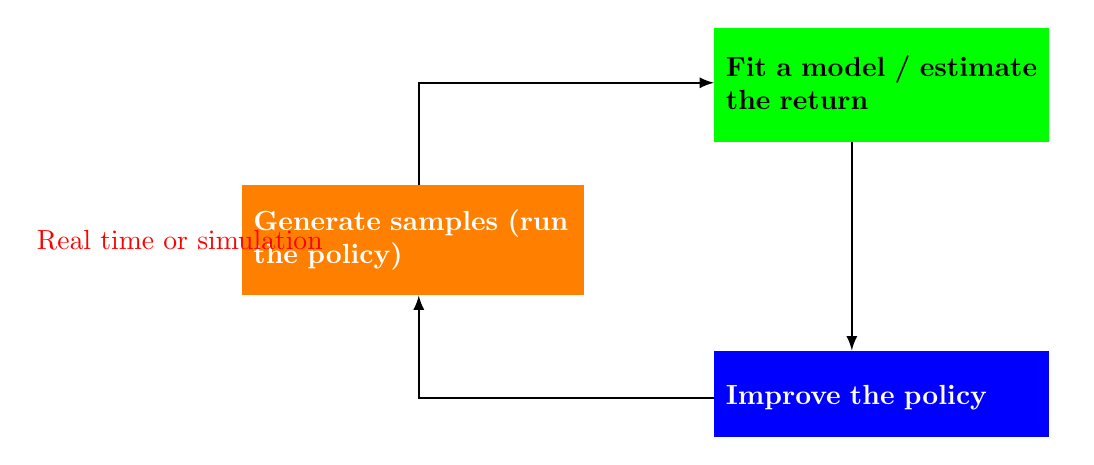
\begin{tikzpicture}
		\fill[green, very thick] (.25,1.25) rectangle (4.5,2.7);
		\fill[blue, very thick] (.25,-1.4) rectangle (4.5,-2.5);
		\fill[orange, very thick] (-5.75,-.7) rectangle (-1.4,.7);
		\node[black, text width=4.2cm] at (2.5,2) {\textbf{Fit a model / estimate the return}};
		\node[white, text width=4.2cm] at (2.5,-2) {\textbf{Improve the policy}};
		\node[white, text width=4.2cm] at (-3.5,0) {\textbf{Generate samples (\ie run the policy)}};
		\node[red, text width=3.7cm] at (-6.5,0) {Real time or simulation};
		\draw[thick, -latex] (2,1.25) -- (2,-1.4);
		\draw[thick, -latex] (.25,-2) -- (-3.5,-2) -- (-3.5,-.7);
		\draw[thick, -latex] (-3.5,.7) -- (-3.5,2) -- (.25,2);
	\end{tikzpicture}
	\caption{Structure of \ac{RL} algorithms.}
	\label{fig:RL-structure}
\end{figure}

\section{Learning resources}
\begin{itemize}
	\item \href{http://rail.eecs.berkeley.edu/deeprlcourse/}{Deep \ac{RL} - CS285, UC Berkeley - Sergey Levine}
	\item \href{http://ai.berkeley.edu/lecture_videos.fhtml}{CS188 Berkeley AI}
	\item Reinforcement learning: An introduction \cite{sutton2018reinforcement}
\end{itemize}

\section{Terminology \& Notation}
\begin{itemize}
	\item Check out \ac{MDP} and \ac{POMDP} in the \href{robotics.pdf}{robotic notes}.
	\item $\textbf{s}_t$ - state
	\item $\textbf{o}_t$ - observation
	\item $\textbf{a}_t$ - action
	\item $\pi_{\theta}(\textbf{a}_t | \textbf{o}_t)$ - policy (or $\pi_{\theta}(\textbf{a}_t | \textbf{s}_t)$ for fully observed scenario)
	\item $r(\textbf{s}_t, \textbf{a}_t)$ - reward or $c(\textbf{s}_t, \textbf{a}_t)$ - cost
	\item $\tau$ - trajectory (as sequence of states and actions)
	\[ p_\theta(\tau) = p_\theta(\textbf{s}_1, \textbf{a}_1, \dots, \textbf{s}_T, \textbf{a}_T) = p(\textbf{s}_1) \prod_{t=1}^{T} \pi_\theta(\textbf{a}_t | \textbf{s}_t) p(\textbf{s}_{t+1} | \textbf{s}_t, \textbf{a}_t) \]
	\item The Q-function is the expectation of total reward, from the q-state $(\textbf{s}_t, \textbf{a}_t)$, under policy $\pi_\theta$.
	\begin{equation}
		Q^\pi (\textbf{s}_t, \textbf{a}_t) = \sum_{t' = t}^{T} \mathbb{E}_{\pi_\theta} \left[ r(\textbf{s}_{t'}, \textbf{a}_{t'}) | \textbf{s}_t, \textbf{a}_t \right]
	\end{equation}
	\item The value function is the expectation of total reward, from the state $\textbf{s}_t$, under policy $\pi_\theta$.
	\begin{equation}
		V^\pi (\textbf{s}_t) = \sum_{t' = t}^{T} \mathbb{E}_{\pi_\theta} \left[ r(\textbf{s}_{t'}, \textbf{a}_{t'}) | \textbf{s}_t \right] = \mathbb{E}_{\textbf{a}_t \sim \pi(\textbf{a}_t | \textbf{s}_t)} Q^\pi (\textbf{s}_t, \textbf{a}_t)
	\end{equation}
\end{itemize}

\begin{figure}[hbt!]
	\centering
	\begin{tikzpicture}[
		roundnode/.style={circle, draw=black!60, very thick, minimum size=7mm}]
		\node[roundnode](o1){$\textbf{o}_1$};
		\node[roundnode](a1)[right=of o1]{$\textbf{a}_1$};
		\node[roundnode](o2)[right=of a1]{$\textbf{o}_2$};
		\node[roundnode](a2)[right=of o2]{$\textbf{a}_2$};
		\node[roundnode](o3)[right=of a2]{$\textbf{o}_3$};
		\node[roundnode](a3)[right=of o3]{$\textbf{a}_3$};		
		\node[roundnode](s1)[below left=of a1]{$\textbf{s}_1$};
		\node[roundnode](s2)[below left=of a2]{$\textbf{s}_2$};	
		\node[roundnode](s3)[below left=of a3]{$\textbf{s}_3$};
		\draw[-latex](o1.east) -- (a1.west) node[midway, above]{$\pi_{\theta}$};
		\draw[-latex](o2.east) -- (a2.west) node[midway, above]{$\pi_{\theta}$};
		\draw[-latex](o3.east) -- (a3.west) node[midway, above]{$\pi_{\theta}$};
		\draw[-latex](s1.east) -- (s2.west) node[midway, below]{$p(\textbf{s}_{t+1} | \textbf{s}_t, \textbf{a}_t)$};
		\draw[-latex](s2.east) -- (s3.west) node[midway, below]{$p(\textbf{s}_{t+1} | \textbf{s}_t, \textbf{a}_t)$};
		\draw[-latex](s1.north) -- (o1.south);
		\draw[-latex](s2.north) -- (o2.south);
		\draw[-latex](s3.north) -- (o3.south);
		\draw[-latex](a1.south east) -- (s2.north west);
		\draw[-latex](a2.south east) -- (s3.north west);
	\end{tikzpicture}
	\caption{The relationship between state $\textbf{s}_t$, observation $\textbf{o}_t$ and action $\textbf{a}_t$.}
\end{figure}

\section{Overview on RL Algorithms}
\ac{RL} problem revolves around maximizing the expectation of total rewards. Thus, we aim to find the \ac{param} to maximize the expected value of the sum of rewards, under the trajectory distribution.
\begin{equation}
	\theta^* = \underset{\theta}{\arg\max}\; \mathbb{E}_{\tau \sim p_\theta(\tau)} \left[ \sum_t r(\textbf{s}_t, \textbf{a}_t) \right]
\end{equation}

There are many methods / algorithms because they have their trade-offs and assumptions:
\begin{itemize}
	\item Sampling efficiency \& stability and ease of use
	\item Stochastic or deterministic
	\item Continuous or discrete
	\item Episode or infinite horizon
\end{itemize}
\tabref{tab:RL-algors} gives an overview and comparison between algorithms.

\section{Challenges}
\begin{itemize}
	\item Humans can learn incredibly quickly
	\item Humans can reuse past knowledge\\
	Transfer learning in Deep \ac{RL} is an open problem
	\item Not clear what the reward function should be
	\item Not clear what the role of prediction should be
\end{itemize}

\begin{landscape}
	\begin{table}[htb!]
		\centering
		\begin{tblr}{colspec={X[0.6]||X|X[1.2]|X|X}, row{1} = {l}}
			& Model-based approaches & Value function fitting methods & Actor-critic algorithms & Policy Gradient \\ \hline\hline
			\textbf{\textit{Sample efficiency}} \newline {\fontsize{8}{0}\selectfont (How many samples do we need to get good policy?)}
			& \SetCell[c=4]{l}{\newline 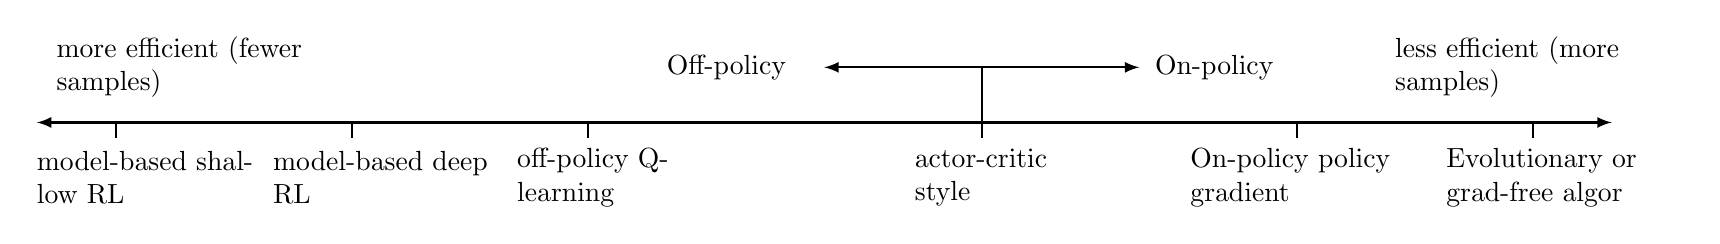
\begin{tikzpicture}[baseline=0]
					\draw[thick,latex-latex] (-10,0) -- (10,0);
					\draw[thick] (-9,0) -- (-9,-0.2);
					\node[text width=3cm] at (-8.5,-.7) {model-based shallow \ac{RL}};
					\draw[thick] (-6,0) -- (-6,-0.2);
					\node[text width=3cm] at (-5.5,-.7) {model-based deep \ac{RL}};
					\draw[thick] (2,0.7) -- (2,0);
					\draw[thick, latex-latex] (0,0.7) -- (4,0.7);
					\draw[thick] (-3,0) -- (-3,-.2);
					\node[text width=3cm] at (-2.4,-.7) {off-policy Q-learning};
					\draw[thick] (2,0) -- (2,-.2);
					\node[text width=2.5cm] at (2.4,-.7) {actor-critic style};
					\draw[thick] (6,0) -- (6,-.2);
					\node[text width=2.7cm] at (6,-.7) {On-policy policy gradient};
					\draw[thick] (9,0) -- (9,-.2);
					\node[text width=3cm] at (9.4,-.7) {Evolutionary or grad-free \ac{algor}};
					\node[text width=4cm] at (0,0.7) {Off-policy};
					\node[text width=4cm] at (6.2,0.7) {On-policy};
					\node[text width=3.5cm] at (-8,.7) {\hlr{more efficient (fewer samples)}};
					\node[text width=3.5cm] at (9,.7) {\hlr{less efficient (more samples)}};
				\end{tikzpicture} \newline\newline - Sometimes, with simulated experiences, we can use \hlr{less efficient} \ac{algor} \newline \hlr{Wall clock time $\neq$ efficiency} \newline - More assumptions, as we go to the left } \\ \hline	
			\SetCell[r=2]{l}{\textbf{\textit{Stability \& ease of use}} \newline {\fontsize{9}{0}\selectfont - Does it converge? \newline - If yes, to what? \newline - Does it \hlr{always} converge?}} & \SetCell[c=4]{l}{\hlr{\ac{RL} is often not \ac{GD}}} \\
			& Model will converge.\newline \hlb{BUT}, better model do \hlr{NOT GUARANTEE} better policy &
			Minimize error of fit \newline At worst case, doesn't optimize anything.\newline Un-provable convergence \newline \hlr{$\Rightarrow$ more like heuristics} & &
			\hlr{is \ac{GD}}\newline least efficient + assumptions \\ \hline				
			\textbf{\textit{Assumption}} &
			By some: episode learning &
			\hlb{Generally}: \newline full observability. \newline By some continuous method: continuity / smoothness & &
			By pure policy gradient methods: \newline \hlb{Often:} episode learning \\ \hline				
			\textbf{\textit{Example}} & 
			- Dyna \newline - Guided policy search &
			- Q-learning \newline - DQN \newline - Temporal difference \newline - Fitted value iteration &
			- \ac{A3C} \newline - \ac{SAC} &
			- REINFORCE \newline - Natural policy gradient \newline - Trusted Region policy optimization\\
		\end{tblr}
		\caption{Different \ac{RL} algorithms.}
		\label{tab:RL-algors}
	\end{table}
\end{landscape}

% !TeX spellcheck = en_US
\chapter{Imitation Learning}

\ac{IL}, \ac{aka} \textit{Behavior Cloning}, \ac{LfD}, essentially, this is \hlb{\underline{supervised learning}}. One problem might arise: applying the learned policy $\pi_{\theta}$ might lead to different action $\textbf{a}_t$, which then leads to different observations and states, comparing to the given dataset: $p_{data}(\textbf{o}_t)~\neq~p_{\pi_{\theta}}(\textbf{o}_t)$. This \hlb{distribution mismatch} can be tackled by adding on-policy data.

\section{DAgger}
\label{sec:dagger}
\ac{dagger} aggregates training data from $p_{\pi_{\theta}}(\textbf{o}_t)$ instead of just $p_{data}(\textbf{o}_t)$. Without \ac{dagger}, it is proven that the error will grow quadratically with the number of time steps $\mathcal{O}(\epsilon T^2)$. \cite{ross2011ais}
\begin{enumerate}
	\item \tikzmark{il1}Train $p_{\pi_{\theta}}(\textbf{o}_t)$ from human data $\mathcal{D} = \{ (\textbf{o}_t, \textbf{a}_t)_i\}$
	\item Run $p_{\pi_{\theta}}(\textbf{o}_t)$ to get data set $\mathcal{D}_\pi = \{\textbf{o}_1, \dots, \textbf{o}_M\}$
	\item Ask human to label $\mathcal{D}_\pi$ with action $\textbf{a}_t$
	\item \tikzmark{il4}Aggregate $\mathcal{D} \leftarrow \mathcal{D} \bigcup \mathcal{D}_\pi$
	\begin{tikzpicture}[overlay,remember picture]
		\draw[very thick, -latex] ([xshift=-7mm,yshift=1mm]pic cs:il4) --++ (-.5,0) |- ([xshift=-7mm,yshift=1mm]pic cs:il1);
	\end{tikzpicture}
\end{enumerate}
The major problem with \ac{dagger} is that it requires human input again in step 3.

\subsection{Recap}
\begin{itemize}
	\item Requires human to annotate the data
	\item Often (but not always) insufficient by itself (distribution mismatch problem)
	\item Sometimes works well
\end{itemize}
\hlb{Problems:}
\begin{itemize}
	\item Non-Markovian behavior
	\item Multimodal behavior
\end{itemize}
\hlb{Solutions:}
\begin{itemize}
	\item Output a mixture of Gaussians
	\item Latent variable models
	\item Auto-regressive discretization (\href{https://www.youtube.com/watch?v=988gLurg01U&list=PL_iWQOsE6TfURIIhCrlt-wj9ByIVpbfGc&index=7}{src})
\end{itemize}

\section{Visual Imitation Learning}
\subsection{Problem Formulation}
\hlb{Problem setting:} given third-person-view images, output sequence of agent actions.
\begin{align}
	O_{human} &= \{ o_{h,0}, o_{h,1}, \dots, o_{h,T} \} && \text{Input: sequence of visual observations}\\
	A_{robot} &= \{ a_{r,0}, a_{r,1}, \dots, a_{r,T} \} && \text{Output: sequence of agent actions}
\end{align}

\subsection{Data Collection}

\begin{itemize}
	\item Kinesthetic teaching: tedious, time consuming labor work. \cite{tykal2016incrementally}
	\item Human teleoperation: expensive and/or complex, but possibly with large amount of rich and scalable data \cite{zhang2018deep}
	\item Demonstration using assistive tools: is simple but works with one specific \ac{ee} at a time \cite{young2020visual}
\end{itemize}

\begin{figure}[hbt!]
	\centering
	\begin{subfigure}[b]{0.25\textwidth}
		\centering
		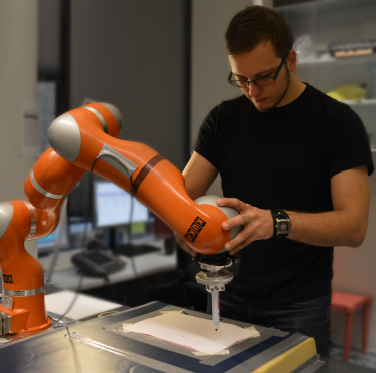
\includegraphics[width=\textwidth]{kinesthetic-teaching.png}
		\caption{Kinesthetic teaching. \cite{tykal2016incrementally}}
	\end{subfigure}
	\hfill
	\begin{subfigure}[b]{0.4\textwidth}
		\centering
		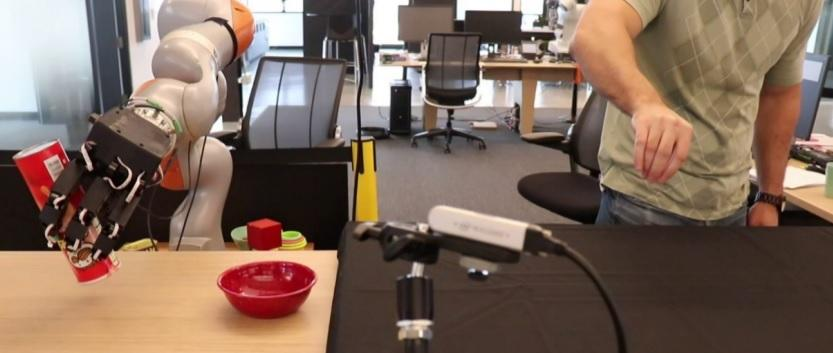
\includegraphics[width=\textwidth]{dexpilot.png}
		\caption{Human teleoperation. \cite{handa2020dexpilot}}
	\end{subfigure}
	\hfill
	\begin{subfigure}[b]{0.3\textwidth}
		\centering
		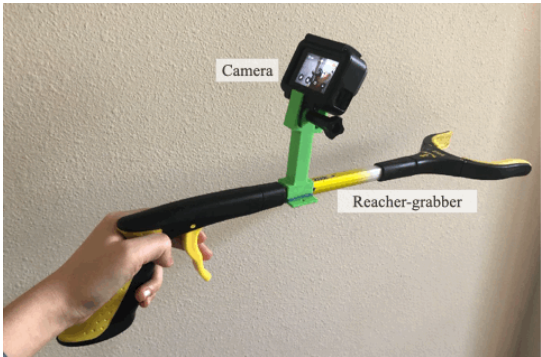
\includegraphics[width=\textwidth]{demoat.png}
		\caption{Assistive tools. \cite{young2020visual}}
	\end{subfigure}
	\caption{Different data collection approaches for visual imitation learning.}
\end{figure}

\subsection{Third Person Visual Imitation}
\citeaustitle{sharma2019third}
\begin{itemize}
	\item The high-level sub-goal generator $ f_{H} $: produces sequence of images, as visual sub-goals, from the images of expert demonstrations
	\begin{align}
		&f_{H}: \mathcal{O}_{rob} \times \mathcal{O}_{h} \times \mathcal{O}_{h} \rightarrow \mathcal{O}_{rob} && \begin{matrix*}[l]
			&\mathcal{O}_{rob} &- \text{robot observation space}\\
			&\mathcal{O}_{h} &- \text{human observation space}
		\end{matrix*}\\
		&f_{H}(o_{r,t}, o_{h,t}, o_{h,t+k}) = o_{r,t+k} && \begin{matrix*}[l]
			&o_{r,t} &- \text{robot observation at time $t$}\\
			&o_{h,t} &- \text{human observation at time $t$}
		\end{matrix*}
	\end{align}
	\item The low-level controller $ \pi_{L} $: produces action plans from the visual sub-goals
	\begin{align}
		&\pi_{L}: \mathcal{O}_{rob} \times \mathcal{O}_{rob} \rightarrow \mathcal{A}_{rob} && \begin{matrix*}[l]
			&\mathcal{O}_{rob} &- \text{robot observation space}\\
			&\mathcal{A}_{rob} &- \text{robot action space}
		\end{matrix*}\\
		&\pi_{L}(o_{r,t}, o_{r,t+k}) = a_{r,t} && \begin{matrix*}[l]
			&o_{r,t} &- \text{robot observation at time $t$}\\
			&a_{r,t} &- \text{robot action at time $t$}
		\end{matrix*}
	\end{align}
\end{itemize}

\hlb{Limitations:} All limitations are probably due to the fact that the authors tried to formulate their goal-generator using the image-to-image translation model \texttt{pix2pix} (\href{https://github.com/pathak22/hierarchical-imitation}{\texttt{github repo}}).
\begin{itemize}
	\item The view points for third-person-view and the robot's first-person-view are \hlr{fixed}.
	\item Even comparing to pix2pix, they have a very strange formulation (personal opinion)
	\item Generate \hlr{low-quality} goal images
	\item Tried, then use \hlr{"bad"} loss functions ($ \mathcal{L}1, \mathcal{L}2 $ loss, \ac{SSIM})
	\item Both high-level and low-level controllers required \hlr{kinesthetic} data collection.
	\item It might also be simpler using optical flow.
	\item Unclear about the baselines comparisons?? 
\end{itemize}

\subsection{One-Shot Visual Imitation Learning with Meta-learning}
\todo{??} \citeaustitle{finn2017one}

\subsection{Others}
There are many works on robotic visual imitation learning. This subsection summarizes their ideas.
\begin{itemize}
	\item Improving generalization with:
	\begin{itemize}
		\item Transformer / Attention network \cite{dasari2020transformers}
		\item Domain randomization \cite{zhou2021manipulator}
		\item Multi-task, instead of one task with many variations \cite{mandi2022towards}
	\end{itemize}
\end{itemize}

\subsection{Proposal}
Perhaps the only way to be able to work with diverse view points and diverse \ac{ee} tools is to formulate interactions with a graph, and with a library of motor primitives for that specific \ac{ee}.

\subsection{References}
\begin{itemize}
	\item \citeaustitle{finn2017one}
	\item \citeaustitle{handa2020dexpilot}
\end{itemize}

% !TeX spellcheck = en_US
\chapter{Policy Gradient}

The Policy Gradient approach has a neural network (\figref{fig:policy-gradient}) to learn and optimize the policy (the blue box in \figref{fig:RL-structure}). This is a model-free \ac{RL} approach. For most model-free \ac{RL} approach, we assume that we don't know the transition model $p(\textbf{s}_{t+1} | \textbf{s}_t, \textbf{a}_t)$ or the initial state \ac{prob} $p(\textbf{s}_1)$. However, we assume that we can interact with the real world to sample the data.

\begin{figure}[hbt!]
	\centering
	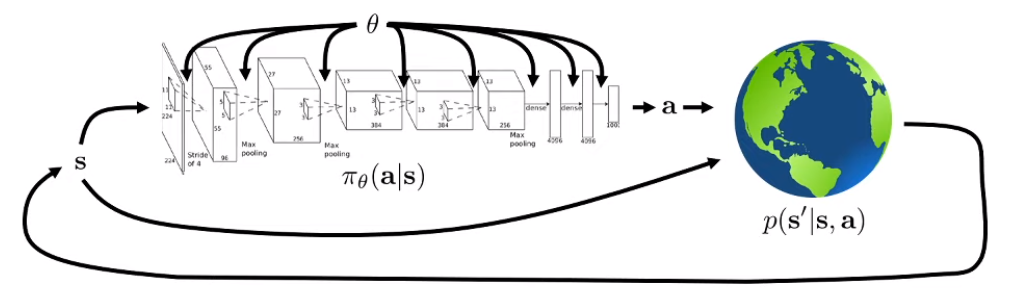
\includegraphics[width=.7\textwidth]{policy-gradient.png}
	\caption{The policy network $\pi_{\theta}(\textbf{a}|\textbf{s})$ with \ac{param} $\theta$. The network takes the current state $\textbf{s}_t$ as input, learn the policy $\pi_{\theta}(\textbf{a}_t|\textbf{s}_t)$ by optimizing \ac{param} $\theta$, and output the action $\textbf{a}_t$.}
	\label{fig:policy-gradient}
\end{figure}

\section{Approach}
\hlb{Goal:} to maximize the expectation of total rewards, which will be denoted as $J(\theta)$
\begin{align}
	\tau & = \{ \textbf{s}_1, \textbf{a}_1, \dots, \textbf{s}_T, \textbf{a}_T \} && \text{denotes the trajectory}\\
	p_\theta(\tau) & = p_\theta(\textbf{s}_1, \textbf{a}_1, \dots, \textbf{s}_T, \textbf{a}_T) && \text{\ac{prob} of the trajectory} \label{eq:traj-prob}\\
	& = p(\textbf{s}_1) \prod_{t=1}^T \pi_{\theta}(\textbf{a}_t | \textbf{s}_t) p(\textbf{s}_{t+1} | \textbf{s}_t, \textbf{a}_t)\\
	\theta^* & = \underset{\theta}{\arg\max} \;\mathbb{E}_{\tau\sim p_\theta(\tau)} \left[ \sum_t r(\textbf{s}_t, \textbf{a}_t) \right] && \text{\ac{RL} goal}\\
	& = \underset{\theta}{\arg\max}\;\mathbb{E}_{(\textbf{s,a})\sim p_\theta(\textbf{s,a})} [r(\textbf{s, a})] && \text{\textbf{infinite} horizon case}\\
	& = \underset{\theta}{\arg\max} \sum_{t=1}^{T} \mathbb{E}_{(\textbf{s}_t,\textbf{a}_t)\sim p_\theta(\textbf{s}_t,\textbf{a}_t)} [r(\textbf{s}_t,\textbf{a}_t)] && \text{\textbf{finite} horizon case}\\
	& = \underset{\theta}{\arg\max} J(\theta)\\
	J(\theta) & = \mathbb{E}_{\tau\sim p_\theta(\tau)} \left[ \sum_{t=1}^T r(\textbf{s}_t, \textbf{a}_t) \right]\\
	& = \mathbb{E}_{\tau\sim p_\theta(\tau)} [r(\tau)] = \int p_\theta(\tau) r(\tau) d\tau
\end{align}

Even though we do not know the initial state \ac{prob} $p(\textbf{s}_1)$ and the transition model $p(\textbf{s}_{t+1} | \textbf{s}_t, \textbf{a}_t)$, we do have the ability to interact with the world and take samples from it. Thus, we can simply take $N$ trajectory samples $\tau_i$ and take the average of them to approximate the expectation of $J(\theta)$. The higher the number of sample trajectories $N$ is, the better the approximation accuracy.
\begin{equation}
	J(\theta) \approx \frac{1}{N} \sum_{i}^N \sum_{t} r(\textbf{s}_{i,t}, \textbf{a}_{i, t}) \qquad \text{sum over samples and time steps}
\end{equation}

\hlb{The Policy Gradient:}
\begin{align}
	\nabla_\theta J(\theta) &= \int \nabla_\theta p_\theta(\tau)r(\tau)d\tau = \int p_\theta(\tau)\nabla_\theta\log p_\theta(\tau)r(\tau)d\tau \label{eq:policy-grad} \\
	&= \mathbb{E}_{\tau\sim p_\theta(\tau)} \left[ \nabla_\theta\log p_\theta(\tau) r(\tau) \right] \label{eq:pg-1}\\
	&= \mathbb{E}_{\tau\sim p_\theta(\tau)} \left[ \left( \sum_{t=1}^{T} \nabla_\theta\log \pi_\theta(\textbf{a}_{t} | \textbf{s}_{t} ) \right) \left( \sum_{t=1}^{T} r(\textbf{s}_{t}, \textbf{a}_{t}) \right) \right] \label{eq:pg-2}
\end{align}
{\color{red} \begin{subequations}
		\begin{empheq}[box=\widefbox]{align}
			\nabla_\theta J(\theta) & \approx \frac{1}{N} \sum_{i=1}^{N} \left[ \left( \sum_{t=1}^{T} \nabla_\theta\log \pi_\theta(\textbf{a}_{i,t} | \textbf{s}_{i,t} ) \right) \left( \sum_{t=1}^{T} r(\textbf{s}_{i,t}, \textbf{a}_{i,t}) \right) \right]\\
			\text{\underline{then}} \quad \theta &\leftarrow \theta + \alpha \nabla_\theta J(\theta)
		\end{empheq}
\end{subequations}}

\hlr{\underline{REMARKS}:}
\begin{itemize}
	\item some what like \ac{MLE}, makes good stuff happen more, bad stuff happens less
	\item Transition in \eqref{eq:policy-grad} happens due to a convenient identity transformation:
	\begin{equation*}
		p_\theta(\tau) \nabla_\theta \log p_\theta(\tau) = p_\theta(\tau) \frac{\nabla_\theta p_\theta(\tau)}{p_\theta(\tau)} = \nabla_\theta p_\theta(\tau)
	\end{equation*}
	\item Taking the $\log$ of $p_\theta(\tau)$ in \eqref{eq:traj-prob} then replacing it into \eqref{eq:pg-1} leads to \eqref{eq:pg-2}
\end{itemize}

\section{Partial Observability}
\begin{align*}
	\nabla_\theta J(\theta) & \approx \frac{1}{N} \sum_{i=1}^{N} \left[ \left( \sum_{t=1}^{T} \nabla_\theta\log \pi_\theta(\textbf{a}_{i,t} | o_{i,t}) \right) \left( \sum_{t=1}^{T} r(\textbf{s}_{i,t}, \textbf{a}_{i,t}) \right) \right]\\
	& \qquad o_{i, t} \rightarrow \underset{\pi_\theta(\textbf{a}_{i,t} | o_{i,t})}{\text{network}} \rightarrow \textbf{a}_{i,t}
\end{align*}
Markov property is not actually used! $\Rightarrow$ can use policy gradient for \ac{POMDP}s without modification

\section{High Variance Problem}
In general, when we add a constant (either positive or negative) to the rewards, the policy should be the same. However, this is not the case for the above derivation of policy gradient. The change of policy distribution varies depends on the value of the total rewards $r(\tau)$. In other words, the problem is \hlr{\underline{HIGH VARIANCE} with $r(\tau)$}.
\begin{itemize}
	\item Different samples $\Rightarrow$ different gradient estimate
	\item For a small finite \ac{no} samples $\Rightarrow$ noisy gradient\\
	(At the beginning, policy $\theta$ is not so good $\Rightarrow$ random action $\Rightarrow$ the not-so-good action results accumulate $\Rightarrow$ high variance in the end)
\end{itemize}

\hlb{Solution:} reducing variance
\begin{itemize}
	\item \textit{Causality:} policy at time $t'$ cannot affect reward at time $t$, when $t'<t$
	\begin{align}
		\Rightarrow\; \nabla_\theta J(\theta) & \approx \frac{1}{N} \sum_{i=1}^{N} \left[ \left( \sum_{t=1}^{T} \nabla_\theta\log \pi_\theta(\textbf{a}_{i,t} | \textbf{s}_{i,t} ) \right) \left( \sum_{\color{red} t'=t}^{T} r(\textbf{s}_{i,t'}, \textbf{a}_{i,t'}) \right) \right]\\
		& \approx \frac{1}{N} \sum_{i=1}^{N} \sum_{t=1}^{T} \nabla_\theta\log \pi_\theta(\textbf{a}_{i,t} | \textbf{s}_{i,t} ) \widehat{Q}_{i,t} \qquad\quad (\widehat{Q}_{i,t} \text{ - the reward to-go})
		\label{eq:Q-value}
	\end{align}
	This leads to smaller variance, because $\widehat{Q}_{i,t}$ is smaller than the total rewards, and the expectation of smaller number has smaller variance.
	\item \textit{Baselines:} the average of total rewards over different trajectories
	\begin{align}
		b &= \frac{1}{N} \sum_{i=1}^{N}r(\tau)\\
		\nabla_\theta J(\theta) & \approx \frac{1}{N} \sum_{i=1}^{N} \nabla_\theta\log \pi_\theta(\tau) [r(\tau)-b]\\
		& {\color{red} r(\tau)-b = Q^\pi(\textbf{s}_t, \textbf{a}_t) - V^\pi(\textbf{s}_t)}
	\end{align}
	It is proven that subtracting the baseline is unbiased in expectation. This is not the best baseline to reduce the variance, but it's simple and good enough.
\end{itemize}

\section{Off-policy Policy Gradient}
Vanilla Policy Gradient is on-policy, since we have $\tau\sim\ p_\theta(\tau)$. This poses a problem, since the neural networks change only a bit with each gradient step. Off-policy Policy Gradient can be derived with \hlr{Important sampling}:
\begin{align}
	\mathbb{E}_{x\sim p(x)}[f(x)] &= \mathbb{E}_{x\sim q(x)} \left[\frac{p(x)}{q(x)}f(x)\right]\\
	\Rightarrow \quad \nabla_{\theta'} J(\theta') & = \mathbb{E}_{\tau \sim p_{\theta}(\tau)} \left[ \frac{\nabla_{\theta'} p_{\theta'}(\tau)}{p_{\theta}(\tau)} r(\tau) \right]\\
	&= \mathbb{E}_{\tau \sim p_{\theta}(\tau)} \left[ \frac{p_{\theta'}(\tau)}{p_{\theta}(\tau)} \nabla_{\theta'}\log p_{\theta'}(\tau) r(\tau) \right]\\
	&\approx \frac{1}{N} \sum_{i=1}^N \sum_{t=1}^T \frac{\pi_{\theta'}(\textbf{a}_{i,t} | \textbf{s}_{i,t})}{\pi_{\theta}(\textbf{a}_{i,t} | \textbf{s}_{i,t})} \nabla_{\theta'} \log \pi_{\theta'} (\textbf{a}_{i,t} | \textbf{s}_{i,t}) \widehat{Q}_{i,t}
\end{align}
with $\theta'$ as the \textit{new} \ac{param} and $\theta$ as the \textit{old} \ac{param}

\section{REINFORCE Algorithm}
\begin{enumerate}
	\item \tikzmark{pg1}Sample $\{\tau_i\}$ from $\pi_\theta(\textbf{a}_t|\textbf{s}_t)$ policy
	\item $\displaystyle \nabla_\theta J(\theta) \approx \frac{1}{N} \sum_{i=1}^{N} \nabla_\theta\log \pi_\theta(\tau) \left(\sum_{t'=t}^{T} r(\textbf{s}_{i,t'}, \textbf{a}_{i, t'})\right)$\\
	\item \tikzmark{pg3}$\theta \leftarrow \theta + \alpha \nabla_\theta J(\theta)$ \qquad\qquad \cite{williams1992jml}
	\begin{tikzpicture}[overlay,remember picture]
		\draw[very thick, -latex] ([xshift=-7mm,yshift=1mm]pic cs:pg3) --++ (-.5,0) |- ([xshift=-7mm,yshift=1mm]pic cs:pg1);
	\end{tikzpicture}
\end{enumerate}

\hlr{Pseudo code:} (\texttt{tensorflow})\\
When coding, use the pseudo loss as a weighted maximum likelihood:
\begin{equation}
	\widetilde{J}(\theta) \approx \frac{1}{N} \sum_{i=1}^{N} \sum_{t=1}^{T} \log \pi_{\theta} (\textbf{a}_{i,t} | \textbf{s}_{i,t} ) \widehat{Q}_{i,t}
\end{equation}
\texttt{logits = policy.predictions(states)}\\
\texttt{negative\_likelihoods = tf.nn.softmax\_cross\_entropy(labels = actions, logits)}\\
\texttt{weighted\_negative\_likelihoods = tf.multiply(negative\_likelihoods, q\_values)}\\
\texttt{loss = tf.reduce\_mean(weighted\_negative\_likelihoods)}\\
\texttt{gradients = loss.gradients(loss, variables)}

with \texttt{q\_values} already taking causality and baselines into account.

\section{Natural Policy Gradient}

Natural Policy gradients, \ac{aka}, covariant policy gradient, apply a trick to change the learning rate for different parameters. The high-level idea is such that some \ac{param} change \ac{prob} a lot more than others. In other words, the vanilla policy gradient apply a constraint on the \ac{param} space rather than the policy space. But with every gradient step, we rather want a constant step in the policy space. \cite{peters2008nn}

\begin{align}
	&\theta' \leftarrow \underset{\theta'}{\arg\max} (\theta'-\theta)^T \nabla_\theta J(\theta) \quad \text{\ac{st} } ||\theta' - \theta||^2 \leq \epsilon \quad \text{(\ac{param} space)}\\
	&\theta' \leftarrow \underset{\theta'}{\arg\max} (\theta'-\theta)^T \nabla_\theta J(\theta) \quad \text{\ac{st} } D(\pi_{\theta'}, \pi_{\theta}) \leq \epsilon \quad \text{(policy space)}
\end{align}

A good choice for $D(\pi_{\theta'}, \pi_{\theta})$ is the \ac{KL}-divergence. To simplify the process, the \ac{KL}-divergence is approximated with Fisher information matrix

\begin{align}
	& D_{KL}(\pi_{\theta'} || \pi_{\theta}) \approx (\theta' - \theta)^T \textbf{F} (\theta' - \theta)\\
	& \textbf{F} = \mathbb{E}_{\pi_{\theta}} [ \nabla_\theta \log\pi_\theta(\textbf{a}|\textbf{s}) \nabla_\theta \log \pi_\theta (\textbf{a}|\textbf{s})^T ] && \text{Fisher information matrix}\\
	& \theta' \leftarrow \underset{\theta'}{\arg\max} (\theta'-\theta)^T \nabla_\theta J(\theta) \quad \text{\ac{st} } ||\theta' - \theta||^2_\textbf{F} \leq \epsilon\\
	& \theta \leftarrow \theta + \alpha \textbf{F}^{-1} \nabla_\theta J(\theta)
\end{align}

\section{References}
\begin{itemize}
	\item \citeaus{peters2008nn}. Reinforcement learning of motor skills with policy gradients.
	\item \citeaus{levine2013icml}. Guided policy search: deep \ac{RL} with importance sampled policy gradient.
	\item \citeausm{schulman2015icml}. Trust region policy optimization: deep \ac{RL} with natural policy gradient and adaptive step size.
	\item \citeausm{schulman2017proximal}. Proximal policy optimization algorithms: deep \ac{RL} with importance sampled policy gradient
\end{itemize}
% !TeX spellcheck = en_US
\chapter{Actor-Critic}
Actor-Critic is kind of hybrid between policy gradient and value function based approach. Compared to deep Policy gradient, deep Actor-Critic has an extra network to learn the value function (the green box in \figref{fig:RL-structure}).
\begin{itemize}
	\item \hlr{the Actor is the policy}
	\item \hlr{the Critic is the value function (\ac{aka} policy evaluation)}
\end{itemize}

\section{Approach}
We continue with the \eqref{eq:Q-value}, where we multiply with the estimate of the expected reward $\widehat{Q}_{i,t}$. The estimate $\widehat{Q}_{i,t}$ is currently calculated as the sum of the reward afterward, in a single run. There are different ways we could go better than that single-sample estimate.

\begin{itemize}
	\item $Q^\pi(\textbf{s}_t, \textbf{a}_t)$: the Q-function, \ac{aka}, the state-action value function, represents the total reward from taking $\textbf{a}_t$ at state $\textbf{s}_t$, the \textit{true expected} reward-to-go.
	\begin{equation}
		Q^\pi(\textbf{s}_t, \textbf{a}_t) = \sum_{t'=t}^T \mathbb{E}_{\pi_{\theta}}[r(\textbf{s}_{t'}, a_{t'})|\textbf{s}_t, \textbf{a}_t]
		\label{eq:q-function}
	\end{equation}
	\item $V^\pi(\textbf{s}_t)$: the state value function represents the total reward from state $\textbf{s}_t$.
	\begin{equation}
		V^\pi(\textbf{s}_t) = \mathbb{E}_{\textbf{a}_t \sim \pi_{\theta}(\textbf{a}_t, \textbf{s}_t)} [Q^\pi(\textbf{s}_t, \textbf{a}_t)]
	\end{equation}
	\item $A^\pi(\textbf{s}_t, \textbf{a}_t)$: the advantage function: represents how much action $\textbf{a}_t$ is better than average
	\begin{equation}
		A^\pi(\textbf{s}_t, \textbf{a}_t) = Q^\pi(\textbf{s}_t, \textbf{a}_t) - V^\pi(\textbf{s}_t)
		\label{eq:a-function}
	\end{equation}
\end{itemize}

Using these value functions, we would have a better estimate for the policy gradients. Thus, we can rewrite the gradient as:
\begin{align}
	\nabla_\theta J(\theta) &= \frac{1}{N} \sum_{i=1}^N\sum_{t=1}^T \nabla_\theta\log\pi_{\theta}( \textbf{a}_{i,t}|\textbf{s}_{i,t} ) A^\pi(\textbf{s}_{i,t}, \textbf{a}_{i,t} )\\
	Q^\pi(\textbf{s}_t, \textbf{a}_t) &= r(\textbf{s}_t, \textbf{a}_t) + \mathbb{E}_{\textbf{s}_{t+1}\sim p(\textbf{s}_{t+1} | \textbf{s}_t, \textbf{a}_t)} V^\pi(\textbf{s}_{t+1}) && \text{(\eqref{eq:q-function})}\\
	&\approx r(\textbf{s}_t, \textbf{a}_t) + V^\pi(\textbf{s}_{t+1}) &&\text{(with 1 sample)}\\
	\Rightarrow \quad A^\pi(\textbf{s}_t, \textbf{a}_t) &\approx r(\textbf{s}_t, \textbf{a}_t) + V^\pi(\textbf{s}_{t+1}) - V^\pi(\textbf{s}_t) && \text{(\eqref{eq:a-function})}	
\end{align}

\begin{figure}[hbt!]
	\centering
	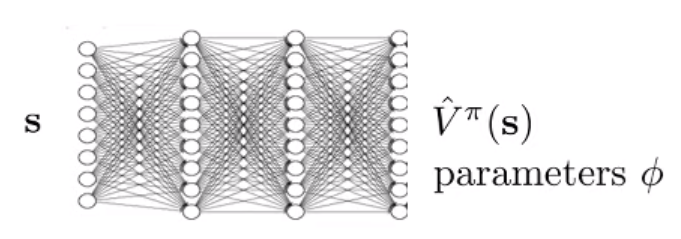
\includegraphics[width=.7\textwidth]{actor-critic.png}
	\caption{The network for value function $V_{\phi}^\pi(s)$ with \ac{param} $\phi$.}
	\label{fig:actor-critic}
\end{figure}

From the above derivation, let just fit the value function $V^\pi(\textbf{s})$ with a neural network. There are two possible approaches:
\begin{itemize}
	\item \hlr{Monte-Carlo:} just as with policy gradient, we approximate by the result from a single sample roll-out.
	\begin{equation}
		V^\pi(\textbf{s}_t) \approx \sum_{t'=t}^T r(\textbf{s}_{t'}, \textbf{a}_{t'})
	\end{equation}
	The average of multiple samples would be a better approximation for the true expectation. However, we could not simply stop at one state within the trajectories and try out different actions. Single sample estimation is still pretty good!
	\begin{align}
		&\text{Better (but not possible)} && V^\pi(\textbf{s}_t) \approx \frac{1}{N} \sum_{i=1}^N \sum_{t'=t}^T r(\textbf{s}_{t'}, \textbf{a}_{t'})\\
		&\text{Training data:} && \{(\textbf{s}_{i,t}, y_{i,t}) \} = \left\{\left(\textbf{s}_{i,t}, \sum_{t'=t}^T r(\textbf{s}_{i,t'}, \textbf{a}_{i,t'})\right)\right\}\\
		&\text{Supervised regression:} && \mathcal{L}(\phi) = \frac{1}{2} \sum_{i} \left|\left| \widehat{V}_{\phi}^{\pi}(\textbf{s}_i) - y_i\right|\right| ^2
	\end{align}
	\item \hlr{Bootstrapped estimate:} use the previous fitted value function
	\begin{align}
		y_{i,t} &= \sum_{t'=t}^{T} \mathbb{E}_{\pi_{\theta}} [r(\textbf{s}_{t'}, a_{t'} | \textbf{s}_{i,t})] &&\text{ideal target}\\
		&\approx r(\textbf{s}_{i,t}, a_{i, t}) + V^{\pi}(\textbf{s}_{i,t+1})\\
		&\approx r(\textbf{s}_{i,t}, a_{i, t}) + \widehat{V}_{\phi}^{\pi}(\textbf{s}_{i,t+1})
	\end{align}
	\begin{align}
		&\text{Training data:} && \{(\textbf{s}_{i,t}, y_{i,t}) \} = \left\{\left(\textbf{s}_{i,t}, r(\textbf{s}_{i,t}, \textbf{a}_{i,t}) + \widehat{V}^\pi_\phi(\textbf{s}_{i,t+1}) \right)\right\}\\
		&\text{Supervised regression:} && \mathcal{L}(\phi) = \frac{1}{2} \sum_{i} \left|\left| \widehat{V}_{\phi}^{\pi}(\textbf{s}_i) - y_i\right|\right| ^2
	\end{align}	
\end{itemize}

\section{Batch Actor-Critic}
\begin{enumerate}
	\item \tikzmark{bac1}Sample $\{\textbf{s}_i, \textbf{a}_i\}$ from $\pi_{\theta}(\textbf{a|s})$
	\item Fit $V_{\phi}^\pi(\textbf{s})$ to sampled reward sums (either Monte-Carlo or bootstrapped estimate)
	\item Evaluate $\widehat{A}^\pi(\textbf{s}_i, \textbf{a}_i) = r(\textbf{s}_i, \textbf{a}_i) + \widehat{V}_\phi^\pi(\textbf{s}_{i'}) - \widehat{V}_\phi^\pi(\textbf{s}_{i})$
	\item $\nabla_\theta J(\theta) \approx \sum \nabla_\theta\log\pi_{\theta}( \textbf{a}_{i}|\textbf{s}_{i} ) \widehat{A}^\pi(\textbf{a}_i, \textbf{s}_i)$
	\item \tikzmark{bac5}$\theta \leftarrow \theta + \alpha \nabla_\theta J(\theta)$
	\begin{tikzpicture}[overlay,remember picture]
		\draw[very thick, -latex] ([xshift=-7mm,yshift=1mm]pic cs:bac5) --++ (-.5,0) |- ([xshift=-7mm,yshift=1mm]pic cs:bac1);
	\end{tikzpicture}
\end{enumerate}
With \hlr{discount factor $\gamma$} $\in [0,1]$ (0.99 works well)\\
3. Evaluate $\widehat{A}^\pi(\textbf{s}_i, \textbf{a}_i) = r(\textbf{s}_i, \textbf{a}_i) + \gamma\widehat{V}_\phi^\pi(\textbf{s}_{i'}) - \widehat{V}_\phi^\pi(\textbf{s}_{i})$ \cite{thomas2014icml}

\section{Online Actor-Critic}
\begin{enumerate}
	\item \tikzmark{oac1}Take action $\textbf{a} \sim \pi_{\theta}(\textbf{a|s})$, get sample $(\textbf{s, a, s'}, r)$
	\item Update $\widehat{V}_\phi^\pi$ using target value $r + \gamma \widehat{V}_\phi^\pi(\textbf{s}')$
	\item Evaluate $\widehat{A}^\pi(\textbf{s, a}) = r(\textbf{s, a}) + \widehat{V}_\phi^\pi(\textbf{s}') - \widehat{V}_\phi^\pi(\textbf{s})$
	\item $\nabla_\theta J(\theta) \approx \nabla_\theta\log\pi_{\theta}(\textbf{a|s}) \widehat{A}^\pi(\textbf{s, a})$
	\item \tikzmark{oac5}$\theta \leftarrow \theta + \alpha \nabla_\theta J(\theta)$
	\begin{tikzpicture}[overlay,remember picture]
		\draw[very thick, -latex] ([xshift=-7mm,yshift=1mm]pic cs:oac5) --++ (-.5,0) |- ([xshift=-7mm,yshift=1mm]pic cs:oac1);
	\end{tikzpicture}
\end{enumerate}
\hlr{Problem:} single batch $\Rightarrow$ need parallel actor-critic (synchronous / asynchronous)

\section{Design Decisions}
\begin{itemize}
	\item Architecture design:
	\begin{table}[hbt!]
		\centering
		\begin{tabular}{c|c}
			Two separate networks & Shared network design\\
			\hline\hline
			$\begin{matrix*}[l]
				\color{Green} + \text{simple and stable}\\
				\color{red} - \text{no shared features between actor \& critic}
			\end{matrix*}$ & $\begin{matrix*}[l]
				\color{Green} + \text{could be more efficient in practice}\\
				\color{red} - \text{two different gradients which need to tuned}
			\end{matrix*}$ \\ 
			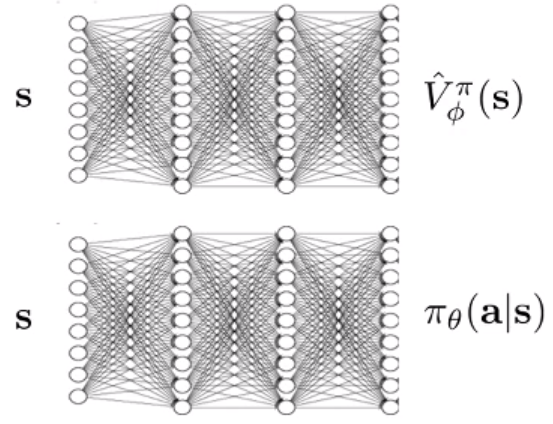
\includegraphics[width=0.3\textwidth]{ac-networks-1.png} &
			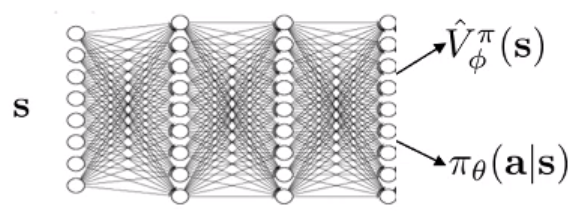
\includegraphics[width=0.5\textwidth]{ac-networks-2.png}
		\end{tabular}
	\end{table}	
	
	\item Critic as state-dependent baselines\\
	Actor-critic: $\begin{matrix*}[l]
		\color{Green}+\text{lower variance (due to critic)}\\
		\color{red}-\text{not unbiased (if the critic is not perfect)}
	\end{matrix*}$
	\[\nabla_\theta J(\theta) \approx \frac{1}{N} \sum_{i=1}^N \sum_{t=1}^T \nabla_\theta\log\pi_{\theta}(\textbf{a}_{i,t}|\textbf{s}_{i,t}) \left( r(\textbf{s}_{i,t}, \textbf{a}_{i,t}) + {\color{red}\gamma\widehat{V}_\phi^\pi(\textbf{s}_{i,t+1}) - \widehat{V}_\phi^\pi(\textbf{s}_{i,t})} \right)\]
	Policy gradient: $\begin{matrix*}[l]
		\color{Green}+ \text{no bias}\\
		\color{red}- \text{higher variance (because of single-sample estimate)}
	\end{matrix*}$
	\[\nabla_\theta J(\theta) \approx \frac{1}{N} \sum_{i=1}^N \sum_{t=1}^T \nabla_\theta\log\pi_{\theta}(\textbf{a}_{i,t}|\textbf{s}_{i,t}) \left( \left( \sum_{t' = t}^T \gamma^{t'-t} r(\textbf{s}_{i,t'}, \textbf{a}_{i,t'}) \right) -b \right)\]
	$\Rightarrow$ Critic as baseline: $\color{Green}\begin{matrix*}[l]
		+ \text{no bias}\\
		+ \text{lower variance (baseline is closer to rewards)}
	\end{matrix*}$
	\[\nabla_\theta J(\theta) \approx \frac{1}{N} \sum_{i=1}^N \sum_{t=1}^T \nabla_\theta\log\pi_{\theta}(\textbf{a}_{i,t}|\textbf{s}_{i,t}) \left( \left( \sum_{t' = t}^T \gamma^{t'-t} r(\textbf{s}_{i,t'}, \textbf{a}_{i,t'}) \right) - {\color{red}\widehat{V}_\phi^\pi(\textbf{s}_{i,t})} \right)\]
	This doesn't lower the variance as much as in the actor-critic algorithm. But it is much lower than using a constant baseline, and it's still unbiased.
	
	\item Control variates: action-dependent baselines \cite{gu2016q}\\
	We could go further with a state dependent baseline, and have a action-and-state-dependent baselines. The variance is now even lower, but it's getting much more complicated.
	\begin{align*}
		&\widehat{A}^\pi(\textbf{s}_t, \textbf{a}_t) = \sum_{t' = t}^\infty \gamma^{t'-t} r(\textbf{s}_{t'}, \textbf{a}_{t'}) - {\color{red} V_\phi^\pi(\textbf{s}_{t})} && \begin{matrix*}[l]
			\color{Green} + \text{no bias (state dependent baseline)}\\
			\color{red} - \text{still high variance (compared to actor-critic)}
		\end{matrix*}\\
		&\widehat{A}^\pi(\textbf{s}_t, \textbf{a}_t) = \sum_{t' = t}^\infty \gamma^{t'-t} r(\textbf{s}_{t'}, \textbf{a}_{t'}) - {\color{red} Q_\phi^\pi(\textbf{s}_{t}, \textbf{a}_{t})} && \begin{matrix*}[l]
			\color{Green} + \text{goes to 0 in expectation if critic is correct}\\
			\color{red} - \text{not correct}
		\end{matrix*}
	\end{align*}
	The second one lead to wrong policy gradient, thus must be corrected with an error term:
	\begin{equation}
		\nabla_\theta J(\theta) \approx \frac{1}{N} \sum_{i=1}^N \sum_{t=1}^T \nabla_\theta\log\pi_{\theta}(\textbf{a}_{i,t}|\textbf{s}_{i,t}) \left( \widehat{Q}_{i,t} - Q^\pi_\phi(\textbf{s}_{i,t}, \textbf{a}_{i,t}) \right) + \frac{1}{N} \sum_{i=1}^N \sum_{t=1}^T \nabla_\theta\mathbb{E}_{\textbf{a}\sim\pi_\theta(\textbf{a}_t | \textbf{s}_{i,t})}[Q^\pi_\phi(\textbf{s}_{i,t}, \textbf{a}_{i,t})]
	\end{equation}
	
	\item Eligibility traces \& $n$-step returns: reduces the bias
	\begin{align}
		&\text{Actor-critic:} &&\widehat{A}_C^\pi(\textbf{s}_t, \textbf{a}_t) = r(\textbf{s}_t, \textbf{a}_t) + \gamma \widehat{V}_\phi^\pi(\textbf{s}_{t+1}) - \widehat{V}_\phi^\pi(\textbf{s}_t) \quad \begin{matrix*}[l]
			{\color{Green} + \text{low variance}}\\
			{\color{red} - \text{but biased}}
		\end{matrix*}\\
		&\text{Monte-Carlo:} &&\widehat{A}_{MC}^\pi(\textbf{s}_t, \textbf{a}_t) = \sum_{t' = t}^\infty \gamma^{t'-t} r(\textbf{s}_{t'}, a_{t'}) - \widehat{V}_\phi^\pi(\textbf{s}_t) \quad\begin{matrix*}[l]
			{\color{Green} + \text{no bias}}\\
			{\color{red} - \text{higher variance}}				
		\end{matrix*}\\
		&\qquad\Rightarrow &&\widehat{A}_n^\pi (\textbf{s}_t, \textbf{a}_t) = \sum_{t'=t}^{\color{red} t+n} \gamma^{t'-t} r(\textbf{s}_{t'}, a_{t'}) - \widehat{V}_\phi^\pi(\textbf{s}_t) + \gamma^n \widehat{V}_\phi^\pi(\textbf{s}_{t+n})
	\end{align}
	Simply put, the further the states are in the future, the higher the variance of those states. \Eg, where would you/the robot be in 5 minutes versus where would you/the robot be in 20 years? The larger $n$ is, the lower the bias, the higher the variance.
	\item Generalized advantage estimation: extension of $n$-step returns\\
	To have many $n$-step returns, then take weighted average of them.	
	\begin{align}
		&\widehat{A}_{GAE}^\pi(\textbf{s}_t, \textbf{a}_t) = \sum_{n=1}^\infty \omega_n \widehat{A}_n^\pi(\textbf{s}_t, \textbf{a}_t), && \omega_n \propto \lambda^{n-1}\\
		\Rightarrow\;&\widehat{A}_{GAE}^\pi(\textbf{s}_t, \textbf{a}_t) = \sum_{t'=t}^\infty (\gamma\lambda)^{t'-t} \delta_{t'}, && \delta_{t'} = r(\textbf{s}_{t'}, \textbf{a}_{t'}) + \gamma \widehat{V}^\pi_\phi(\textbf{s}_{t'+1}) - \widehat{V}_\phi^\pi(\textbf{s}_{t'})
	\end{align}
\end{itemize}

\section{References}
\begin{itemize}
	\item \citeaus{sutton1999policy}. Policy gradient methods for reinforcement learning with function approximation.
	\item \citeausm{mnih2016icml}. Asynchronous methods for deep reinforcement learning.
	\item \citeausm{schulman2015high}. High-dimensional continuous control using generalized advantage estimation.
	\item \citeausm{gu2016q}. Q-prop: Sample-efficient policy gradient with an off-policy critic.
\end{itemize}
% !TeX spellcheck = en_US
\chapter{Value Function Based Algorithms}
\section{Approach}
Knowing the value functions, we could just remove the policy gradient completely. The advantage function $A^\pi(\textbf{s}_t, \textbf{a}_t)$ tells how much better is $\textbf{a}_t$ than the average action according to policy $\pi$, regardless of what $\pi(\textbf{a}_t | \textbf{s}_t)$ is. We could have a policy $\pi'$ by simply choosing the current best action. $\pi'$ would be as good as $\pi$ (probably better).

\hlb{High-level idea for Policy Iteration:}
\begin{enumerate}
	\item \tikzmark{pi1}Evaluate $A^\pi(s,a)$ (policy evaluation)
	\item \tikzmark{pi2}Set $\pi \leftarrow \pi'$
	\begin{tikzpicture}[overlay,remember picture]
		\draw[very thick, -latex] ([xshift=-7mm,yshift=1mm]pic cs:pi2) --++ (-.5,0) |- ([xshift=-7mm,yshift=1mm]pic cs:pi1);
	\end{tikzpicture}
\end{enumerate}
\begin{equation}
	\pi'(\textbf{a}_t|\textbf{s}_t) = \begin{cases}
		1 \qquad \text{if } \textbf{a}_t = \underset{\textbf{a}_t}{\arg\max}\; A^\pi(\textbf{s}_t, \textbf{a}_t)\\
		0 \qquad \text{otherwise}
	\end{cases}
\end{equation}

\section{Policy Iteration with Dynamic Programming}
\hlb{Dynamic Programming}:
\begin{itemize}
	\item Assume we know $p(\textbf{s}'|\textbf{s,a})$
	\item $\textbf{s}$ and $\textbf{a}$ are both discrete and small
	\item $V^\pi(\textbf{s})$  can be stored in a lookup table
	\item $\mathcal{T}$ is a tensor
\end{itemize}

\hlb{Algorithm:}
\begin{enumerate}
	\item \tikzmark{pidp1}$V^\pi(\textbf{s}) \leftarrow r(\textbf{s}, \pi(\textbf{s})) + \gamma\mathbb{E}_{\textbf{s}'\sim p(\textbf{s}'|\textbf{s},\pi(\textbf{s}))} [V^\pi(\textbf{s}')]$
	\item \tikzmark{pidp2}Set $\pi \leftarrow \pi'$
	\begin{tikzpicture}[overlay,remember picture]
		\draw[very thick, -latex] ([xshift=-7mm,yshift=1mm]pic cs:pidp2) --++ (-.5,0) |- ([xshift=-7mm,yshift=1mm]pic cs:pidp1);
	\end{tikzpicture}
\end{enumerate}

\section{Value Iteration Algorithm}
\label{sec:value-iteration}
Since $\underset{\textbf{a}_t'}{\arg\max}\; A^\pi(\textbf{s}_t, \textbf{a}_t) = \underset{\textbf{a}_t'}{\arg\max}\; Q^\pi(\textbf{s}_t, \textbf{a}_t)$, we can simplify above \ac{algor}:
\begin{enumerate}
	\item \tikzmark{vi1}Set $Q^\pi(\textbf{s, a}) \leftarrow r(\textbf{s, a}) + \gamma\mathbb{E}[V^\pi(\textbf{s}')]$
	\item \tikzmark{vi2}Set $V^\pi(\textbf{s}) \leftarrow \underset{\textbf{a}}{\max}\; Q^\pi(\textbf{s, a})$
	\begin{tikzpicture}[overlay,remember picture]
		\draw[very thick, -latex] ([xshift=-7mm,yshift=1mm]pic cs:vi2) --++ (-.5,0) |- ([xshift=-7mm,yshift=1mm]pic cs:vi1);
	\end{tikzpicture}
\end{enumerate}

\section{Fitted Value Iteration}
The above two approaches still have a table to fit the value functions. For larger state space (either continuous or discrete), when facing the curse of dimensionality (for \textbf{$s$}), we shall use neural network to evaluate the value functions.
\begin{enumerate}
	\item \tikzmark{fvi1}$\textbf{y}_i \leftarrow \underset{\textbf{a}_i}{\max}\; r(\textbf{s}_i, \textbf{a}_i) + \gamma\mathbb{E}\left[ V_{\phi}(\textbf{s}_i') \right]$
	\item \tikzmark{fvi2}$\phi \leftarrow \underset{\phi}{\arg\min}\;\frac{1}{2} \sum_{i} ||V_{\phi}(\textbf{s}_i) - \textbf{y}_i||^2$
	\begin{tikzpicture}[overlay,remember picture]
		\draw[very thick, -latex]
		([xshift=-7mm,yshift=1mm]pic cs:fvi2) --++ (-.5,0) |-
		([xshift=-7mm,yshift=1mm]pic cs:fvi1);
	\end{tikzpicture}
\end{enumerate}
\begin{figure}[hbt!]	
	\centering
	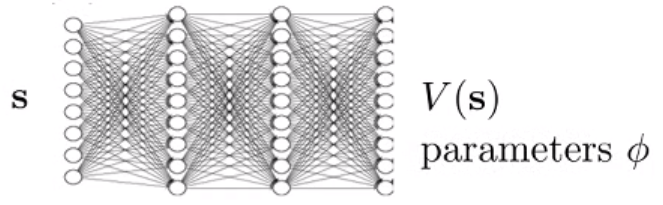
\includegraphics[width=.5\textwidth]{fitted-value-iteration.png}
	\caption{The network for value function $V_{\phi}(s)$ with \ac{param} $\phi$.}
	\label{fig:fitted-value-iteration}
\end{figure}
\hlb{Problem:} still need to know transition dynamic.

\section{Fully fitted Q-Iteration}
Policy evaluation:
\begin{itemize}
	\item $V^\pi(\textbf{s}) \leftarrow r(\textbf{s}, \pi(\textbf{s})) + \gamma\mathbb{E}_{\textbf{s}'\sim p(\textbf{s}'|\textbf{s},\pi(\textbf{s}))} [V^\pi(\textbf{s}')]$ needs to know the transition models
	\item $Q^\pi(\textbf{s, a}) \leftarrow r(\textbf{s, a}) + \gamma\mathbb{E}_{\textbf{s}'\sim p(\textbf{s}'|\textbf{s, a})} [Q^\pi(\textbf{s}', \pi(\textbf{s}'))]$ needs only a sample tuple $\{\textbf{s, a, s}'\}$
\end{itemize}
Replacing since $\mathbb{E}[V(\textbf{s}_i')] \approx \underset{\textbf{a}'}{\max}\; Q_\phi(\textbf{s}_i', \textbf{a}_i')$ into fitted value iteration algorithm, we have Fully fitted Q-iteration:\\
{
	1. \tikzmark{ffqi1}Collect dataset: $\{(\textbf{s}_i, \textbf{a}_i, \textbf{s}_i', r_i)\}$ using some policy\\
	\tab 2. \tikzmark{ffqi2}Set $\textbf{y}_i \leftarrow r(\textbf{s}_i, \textbf{a}_i) + \gamma \underset{\textbf{a}_i'}{\max}\; Q_\phi (\textbf{s}_i', \textbf{a}_i')$\\
	\tab 3. \tikzmark{ffqi3}Set $\phi \leftarrow \underset{\phi}{\arg\min}\; \frac{1}{2} \sum_{i} || Q_{\phi}(\textbf{s}_i, \textbf{a}_i) - \textbf{y}_i ||^2$
	\begin{tikzpicture}[overlay,remember picture]
		\draw[very thick, -latex]
		([xshift=-7mm,yshift=1mm]pic cs:ffqi3) --++ (-.5,0) |-
		([xshift=-7mm,yshift=1mm]pic cs:ffqi2);
		\draw[very thick, -latex]
		([xshift=-7mm,yshift=0mm]pic cs:ffqi3) --++ (-1.2,0) |-
		([xshift=-5mm,yshift=1mm]pic cs:ffqi1);
		\node at ([xshift=-14mm,yshift=7mm]pic cs:ffqi3) {\fontsize{10}{0}\selectfont \rotatebox{90}{$K \times$}};
	\end{tikzpicture}
}

\begin{figure}[hbt!]
	\centering
	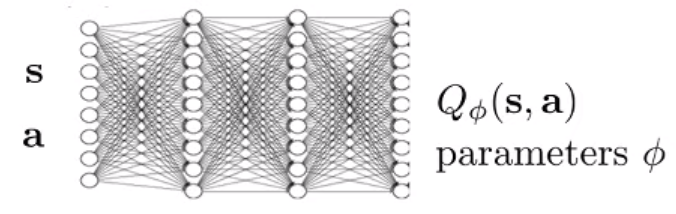
\includegraphics[width=.5\textwidth]{fully-fitted-q-iteration.png}
	\caption{The network for Q-value function $Q_{\phi}(s,a)$ with \ac{param} $\phi$.}
	\label{fig:fully-fitted-q-iteration}
\end{figure}
$\begin{matrix*}[l]
	\color{Green}+ \text{Off-policy (unlike actor-critic)}\\
	\color{Green}+\text{Single network, no high-variance policy gradient}\\
	\color{red}- \text{Not really converge}
\end{matrix*}$

\section{Online Q-Iteration Algorithm}
\begin{enumerate}
	\item \tikzmark{oqi1}Take some action $\textbf{a}_i$ and observe $(\textbf{s}_i, \textbf{a}_i, \textbf{s}_i', r_i)$ \qquad\hlr{1 sample off policy}
	\item $\textbf{y}_i \leftarrow r(\textbf{s}_i, \textbf{a}_i) + \gamma\underset{\textbf{a}_i'}{\max}\; Q_\phi(\textbf{s}_i', \textbf{a}_i')$
	\item \tikzmark{oqi3}$\displaystyle\phi \leftarrow \phi - \alpha\frac{dQ_\phi}{d\phi}(\textbf{s}_i, \textbf{a}_i)\left[ Q_\phi(\textbf{s}_i, \textbf{a}_i) - \textbf{y}_i \right]$  \qquad\qquad\hlr{1 gradient step}
	\begin{tikzpicture}[overlay,remember picture]
		\draw[very thick, -latex]
		([xshift=-7mm,yshift=1mm]pic cs:oqi3) --++ (-.5,0) |-
		([xshift=-7mm,yshift=1mm]pic cs:oqi1);
	\end{tikzpicture}
\end{enumerate}
\hlb{Problems:}
\begin{itemize}
	\item Sequential states are strongly correlated $\Rightarrow$ Replay buffer
	\item Target value is always changing $\Rightarrow$ Target network
\end{itemize}

\section{Exploration vs Exploitation}
\begin{itemize}
	\item Epsilon greedy
	\begin{equation}
		\pi(\textbf{a}_t|\textbf{s}_t) = \begin{cases}
			1-\epsilon \quad\qquad \text{if } \textbf{a}_t = \underset{\textbf{a}_t}{\arg\max}\; A^\pi(\textbf{s}_t, \textbf{a}_t)\\
			\displaystyle \frac{\epsilon }{|\mathcal{A}|-1} \qquad \text{otherwise}
		\end{cases}
	\end{equation}
	\item Boltzmann exploration \hlr{(very large or continuous action-space)}
	\begin{equation}
		\pi(\textbf{a}_t | \textbf{s}_t) \propto \exp (Q_\phi(\textbf{s}_t, \textbf{a}_t))
	\end{equation}
\end{itemize}

\section{Q-learning}
Q-learning with replay buffer $\mathcal{B}$ and target network $\phi'$:\\
{1. \tikzmark{ql1}Save target network \ac{param} $\phi' \leftarrow \phi$\\
	\tab 2. \tikzmark{ql2}Collect dataset $\{(\textbf{s}_i, \textbf{a}_i, \textbf{s}_i', r_i) \}$ using some policy, add it to $\mathcal{B}$\\
	\tab\tab 3. \tikzmark{ql3}Sample a batch $(\textbf{s}_i, \textbf{a}_i, \textbf{s}_i', r_i)$ from $\mathcal{B}$\\
	\tab\tab 4. \tikzmark{ql4}$\displaystyle\phi \leftarrow \phi - \alpha\sum_{i} \frac{dQ_\phi}{d\phi}(\textbf{s}_i, \textbf{a}_i)\left( Q_\phi(\textbf{s}_i, \textbf{a}_i) - \left[ r(\textbf{s}_i, \textbf{a}_i) + \gamma\underset{a'}{\max}\; Q_{\phi'}(\textbf{s}_i', \textbf{a}_i') \right]\right)$\\
	$K \in [1, 4], N \approx 10,000$
	\begin{tikzpicture}[overlay,remember picture]
		\draw[very thick, -latex]
		([xshift=-7mm,yshift=2mm]pic cs:ql4) --++ (-.5,0) |-
		([xshift=-7mm,yshift=1mm]pic cs:ql3);
		\draw[very thick, -latex]
		([xshift=-7mm,yshift=1mm]pic cs:ql4) --++ (-1.2,0) |-
		([xshift=-5mm,yshift=1mm]pic cs:ql2);
		\draw[very thick, -latex]
		([xshift=-7mm,yshift=0mm]pic cs:ql4) --++ (-2.2,0) |-
		([xshift=-5mm,yshift=1mm]pic cs:ql1);
		\node at ([xshift=-14mm,yshift=5mm]pic cs:ql4) {\fontsize{10}{0}\selectfont \rotatebox{90}{$K \times$}};
		\node at ([xshift=-22mm,yshift=2mm]pic cs:ql3) {\fontsize{10}{0}\selectfont \rotatebox{90}{$N \times$}};
\end{tikzpicture}}

\section{Deep Q-learning}
\label{sec:dql}
\begin{enumerate}
	\item \tikzmark{dql1}Take some action $\textbf{a}_i$ and observe $(\textbf{s}_i, \textbf{a}_i, \textbf{s}_i', r_i)$, add it to $\mathcal{B}$
	\item Sample mini-batch $\{(\textbf{s}_j, \textbf{a}_j, \textbf{s}_j', r_j) \}$ from $\mathcal{B}$ uniformly
	\item Compute $y_j = r_j + \gamma \underset{\textbf{a}_j'}{\max} Q_{\phi'}(\textbf{s}_j', \textbf{a}_j')$ using \textit{target} network $Q_{\phi'}$
	\item $\phi \leftarrow \phi - \alpha \sum_j \frac{dQ_\phi}{d\phi}(\textbf{s}_j, \textbf{a}_j) \left( Q_{\phi}(\textbf{s}_j, \textbf{a}_j) - y_j \right)$
	\item \tikzmark{dql5}Update $\phi'$: copy $\phi$ every $N$ steps
	\begin{tikzpicture}[overlay,remember picture]
		\draw[very thick, -latex]
		([xshift=-7mm,yshift=1mm]pic cs:dql5) --++ (-.5,0) |-
		([xshift=-7mm,yshift=1mm]pic cs:dql1);
	\end{tikzpicture}
\end{enumerate}
The above \textit{"Classic"} \ac{DQN} is essentially Q-learning with $K=1$ \cite{mnih2015human}

Improving \ac{DQN}:
\begin{itemize}
	\item Alternative: Step 5. Update $\phi' \leftarrow \tau\phi' + (1-\tau)\phi, \quad \tau = 0.999$ (Polyak averaging)
	\item Double Q-learning: \hlr{helps a lot, solve over-estimate problem, no downside}\\
	\hlr{$\Rightarrow$ should always use}
	\begin{align}
		&\text{Standard Q-learning:} && y = r + \gamma Q_{\phi'}\left( s', \underset{a'}{\arg\max} Q_{\color{red} \phi'}(s', a') \right)\\
		&\text{Double Q-learning:} && y = r + \gamma Q_{\phi'}\left( s', \underset{a'}{\arg\max} Q_{\color{red} \phi}(s', a') \right)
	\end{align}
	\item Multi-Step returns: \hlr{helps a lot, have DOWNSIDE $\Rightarrow$ frequently use} \cite{munos2016safe}
	\begin{align}
		& \text{Q-learning target:} && y_{i,t} = r_{i,t} + \gamma\; \underset{a_{i, t+1}}{\max} Q_{\phi'}(\textbf{s}_{i, t+1}, a_{i, t+1})\\
		& \text{Multi-step target:} && y_{i,t} = \sum_{t'=t}^{t+N-1} \gamma^{t'-t} r_{i,t'} + \gamma^N \underset{a_{i, t+N}}{\max} Q_{\phi'}(\textbf{s}_{i, t+N}, a_{i, t+N})
	\end{align}
	$\begin{matrix*}[l]
		\color{Green} + \text{less biased target values when Q-values are inaccurate}\\
		\color{Green} + \text{typically faster learning, especially early on}\\
		\color{red} - \text{Only actually CORRECT when learning on-policy}
	\end{matrix*}$
\end{itemize}

\section{Q-learning with continuous action-space}
\todo{}

\section{Tips for Q-learning}
\begin{itemize}
	\item Large replay buffer helps improve stability (1 Million).
	\item Apply Prioritized Experience Replay \cite{schaul2015prioritized}
	\item It takes time, be patient - might be no better than random for a while
	\item Start with high exploration $\Rightarrow$ gradually reduce
	\item Bellman error gradient can be quite large $\Rightarrow$ clip gradients / use Huber loss
	\begin{equation}
		L(x) = \begin{cases}
			\frac{x^2}{2} \quad \text{if } |x| \leq \delta\\
			\delta|x| - \frac{\delta^2}{2} \quad \text{otherwise}
		\end{cases} \qquad \text{(Huber loss)}
	\end{equation}
	\item Run multiple random seeds, it's very \hlb{inconsistent} between runs.	
\end{itemize}

\section{Policy Gradient as Policy Iteration}
\todo{math stuffs}

\section{References}
\begin{itemize}
	\item \citeaustitle{watkins1989learning}
	\item \citeaustitle{riedmiller2005neural}
	\item \citeaustitle{lange2010deep}
	\item \citeaustitle{mnih2015human}
	\item \citeaustitle{van2016deep}
	\item \citeaustitle{lillicrap2015continuous}
	\item \citeaustitle{gu2016continuous}
	\item \citeaustitle{wang2016dueling}
	\item \citeaustitle{kalashnikov2018qt}
\end{itemize}
% !TeX spellcheck = en_US
\chapter{Optimal Control}
\label{sec:optimal-control}
Prior approaches are all model-free algorithms. They either assume the dynamics model is unknown or don't even attempt to learn it. On the other hands, there are times that we either do know the dynamics transition or can learn it. \hlr{Knowing the dynamics model actually does make thing easier.} These section is about what we do, how to plan through the action sequence to maximize the reward, \hlr{IF we \underline{already know} the model.}

\begin{itemize}
	\item Deterministic case vs Stochastic:
	\begin{align}
		&\textbf{a}_1, \dots, \textbf{a}_T 	= \underset{\textbf{a}_1, \dots, \textbf{a}_T}{\arg\max} \sum_{t=1}^T r(\textbf{s}_t, \textbf{a}_t) \quad \text{\ac{st} } \textbf{s}_{t+1} = f(\textbf{s}_t, \textbf{a}_t) \quad \text{(Deterministic case)}\\
		&\textbf{a}_1, \dots, \textbf{a}_T = \underset{\textbf{a}_1, \dots, \textbf{a}_T}{\arg\max}\; \mathbb{E} \left[ \sum_t r(\textbf{s}_t, \textbf{a}_t) | \textbf{a}_1, \dots, \textbf{a}_T \right] \quad \text{(Stochastic case)}\\
		&p_\theta(\textbf{s}_1, \dots, \textbf{s}_T | \textbf{a}_1, \dots, \textbf{a}_T) = p(\textbf{s}_1) \prod_{t=1}^T p(\textbf{s}_{t+1} | \textbf{s}_t, \textbf{a}_t) \quad \text{(stochastic dynamics)}
	\end{align}
	\item Open-loop case vs Closed-loop:\\
	Open-loop case: we are only given $\textbf{s}_1$ and have to plan through the whole sequence of actions $\textbf{a}_1, \dots, \textbf{a}_T$. In deterministic case, it's still possible to come up with a good action plan. But for stochastic case, the randomness would probably drive us to a bad result. Closed-loop case: we plan once action $\textbf{a}_t$ at a time and observe the state transition $\textbf{s}_{t+1}$
\end{itemize}

\section{Open-Loop Planning}
Maximize objective through sequence of actions:
\begin{equation}
	\textbf{a}_1, \dots, \textbf{a}_T = \underset{\textbf{a}_1, \dots, \textbf{a}_T}{\arg\max} J(\textbf{a}_1, \dots, \textbf{a}_T) \quad\Rightarrow\quad \textbf{A} = \underset{\textbf{A}}{\arg\max} J(\textbf{A})
\end{equation}

Some stochastic optimization:
\begin{itemize}
	\item Guess and Check (\hlb{Random Shooting Method})
	\begin{enumerate}
		\item Pick $\textbf{A}_1, \dots, \textbf{A}_N$ from some distribution (\eg, uniform)
		\item Choose $\textbf{A}_i$ based on $\underset{i}{\arg\max}J(\textbf{\textbf{A}}_i)$
	\end{enumerate}
	\item \ac{CEM}
	\begin{enumerate}
		\item \tikzmark{cem1}Sample $\textbf{A}_1, \dots, \textbf{A}_N$ from $p(\textbf{A})$
		\item Evaluate $J(\textbf{A}_1), \dots, J(\textbf{A}_N)$
		\item Pick $M$ \textit{elites} $\textbf{A}_{i_1}, \dots, \textbf{A}_{i_M}$ with highest values $M<N$ (usually $10\%$)
		\item \tikzmark{cem4}Refit $p(\textbf{A})$ to the elites $\textbf{A}_{i_1}, \dots, \textbf{A}_{i_M}$
		\begin{tikzpicture}[overlay,remember picture]
			\draw[very thick, -latex]
			([xshift=-7mm,yshift=1mm]pic cs:cem4) --++ (-.5,0) |-
			([xshift=-7mm,yshift=1mm]pic cs:cem1);
		\end{tikzpicture}
	\end{enumerate}
	\note Check out CMA-ES (\ac{CEM} with momentum)
\end{itemize}
The two above approaches are:
\[\begin{matrix*}[l]
	\color{Green}+ \text{very fast if parallelized}\\
	\color{Green}+ \text{extremely simple}\\
	\color{red}- \text{very harsh dimensionality limit}\\
	\color{red}- \text{only open-loop planning}
\end{matrix*}\]

\begin{itemize}
	\item Discrete case: \ac{MCTS} \cite{browne2012survey}
	\begin{enumerate}
		\item \tikzmark{mcts1}Find a leaf $s_l$ using $TreePolicy(s_1)$
		\item Evaluate the leaf using $DefaultPolicy(s_l)$
		\item \tikzmark{mcts3}Update all values in tree between $s_1$ and $s_l$, take the best action from $s_1$.
		\begin{tikzpicture}[overlay,remember picture]
			\draw[very thick, -latex]
			([xshift=-7mm,yshift=1mm]pic cs:mcts3) --++ (-.5,0) |-
			([xshift=-7mm,yshift=1mm]pic cs:mcts1);
		\end{tikzpicture}
		
		UCT Tree Policy($s_t$): if $s_t$ is not fully expanded, choose new $a_t$, else choose child with the highest Score($s_{t+1}$)
		\[\displaystyle Score(s_t) = \frac{Q(s_t)}{N(s_t)} + 2C\sqrt{\frac{2\ln N (s_{t-1})}{N(s_t)}}\]
		With $Q(s_t)$ as the reward, $N(s_t)$ as the \ac{no} times the leaf is visited.
	\end{enumerate}
\end{itemize}

\section{Trajectory Optimization with Derivatives}
\label{sec:lqr}
Derivatives are hard to come by, but SOMETIMES you \textbf{CAN}, through Physics equation.
\begin{align}
	&\underset{\textbf{u}_1, \dots, \textbf{u}_T}{\min}\; \sum_{t=1}^T c(\textbf{x}_t, \textbf{u}_t) \qquad \text{\ac{st} } \textbf{\textbf{x}}_t = f(\textbf{\textbf{x}}_{t-1}, \textbf{\textbf{u}}_{t-1})\\
	= &\underset{\textbf{u}_1, \dots, \textbf{u}_T}{\min}\; c(\textbf{x}_1, \textbf{u}_1) + c(f(\textbf{x}_1, ,\textbf{u}_1), \textbf{u}_2) + \dots + c(f(f(\dots)\dots), \textbf{u}_T)
\end{align}

\note Shooting methods \ac{vs} collocation:
\begin{itemize}
	\item Shooting methods: optimize over actions only
	\[\underset{\textbf{u}_1, \dots, \textbf{u}_T}{\min}\; c(\textbf{x}_1, \textbf{u}_1) + c(f(\textbf{x}_1, ,\textbf{u}_1), \textbf{u}_2) + \dots + c(f(f(\dots)\dots), \textbf{u}_T)\]
	tends to be very sensitive with early actions and leads to numerical instability.
	\item Collocation: optimize over actions and states, with constraints
	\[\underset{\textbf{u}_1, \dots, \textbf{u}_T, \textbf{x}_1, \dots, \textbf{x}_T}{\min}\; \sum_{t=1}^T c(\textbf{x}_t, \textbf{u}_t) \qquad \text{\ac{st} } \textbf{\textbf{x}}_t = f(\textbf{\textbf{x}}_{t-1}, \textbf{\textbf{u}}_{t-1})\]
\end{itemize}

\hlb{Linear case: \ac{LQR}}: $f(\cdot)$ has special structure.
\begin{align}
	f(\textbf{x}_t, \textbf{u}_t) &= \textbf{F}_t \begin{bmatrix}
		\textbf{x}_t\\
		\textbf{u}_t
	\end{bmatrix} + \textbf{f}_t && \text{\hlr{\dunderline{linear} dynamics}}\\
	c(\textbf{x}_t, \textbf{u}_t) &= \frac{1}{2} \begin{bmatrix}
		\textbf{x}_t\\
		\textbf{u}_t
	\end{bmatrix}^T \textbf{C}_t \begin{bmatrix}
		\textbf{x}_t\\
		\textbf{u}_t
	\end{bmatrix} + \begin{bmatrix}
		\textbf{x}_t\\
		\textbf{u}_t
	\end{bmatrix}^T \textbf{c}_t && \text{\hlr{\dunderline{quadratic} cost}}\\
	\textbf{C}_T &= \begin{bmatrix}
		\textbf{C}_{\textbf{x}_T, \textbf{x}_T} & \textbf{C}_{\textbf{x}_T, \textbf{u}_T}\\
		\textbf{C}_{\textbf{u}_T, \textbf{x}_T} & \textbf{C}_{\textbf{u}_T, \textbf{u}_T}
	\end{bmatrix}; \quad \textbf{c}_T = \begin{bmatrix}
		c_{\textbf{x}_T}\\
		c_{\textbf{u}_T}
	\end{bmatrix}
\end{align}
\note \ac{LQR} and its extensions are also an open-loop plannings.

Solve for $\textbf{u}_T$ only:
\begin{align}
	&Q(\textbf{x}_T, \textbf{u}_T) = const + \frac{1}{2} \begin{bmatrix}
		\textbf{x}_t\\
		\textbf{u}_t
	\end{bmatrix}^T \textbf{C}_T \begin{bmatrix}
		\textbf{x}_t\\
		\textbf{u}_t
	\end{bmatrix} + \begin{bmatrix}
		\textbf{x}_t\\
		\textbf{u}_t
	\end{bmatrix}^T \textbf{c}_T \label{eq:lqr-1}\\
	&\text{Set } \nabla_{\textbf{u}_T} Q(\textbf{x}_T, \textbf{u}_T) = \textbf{C}_{\textbf{u}_T, \textbf{x}_T} \textbf{x}_T + \textbf{C}_{\textbf{u}_T, \textbf{u}_T} \textbf{u}_T + \textbf{c}_{\textbf{u}_T}^T = 0\\
	\Rightarrow\quad &\textbf{u}_T = - \textbf{C}^{-1}_{\textbf{u}_T, \textbf{u}_T} (\textbf{C}_{\textbf{u}_T, \textbf{x}_T}.\textbf{x}_T + \textbf{c}_{\textbf{u}_T}) = \textbf{K}_T \textbf{x}_T + \textbf{k}_T \label{eq:lqr-2}\\
	&\textbf{K}_T = - \textbf{C}^{-1}_{\textbf{u}_T, \textbf{u}_T} \textbf{C}_{\textbf{u}_T, \textbf{x}_T}\\
	&\textbf{k}_T = - \textbf{C}^{-1}_{\textbf{u}_T, \textbf{u}_T} \textbf{c}_{\textbf{u}_T}\\
\end{align}

Replace \eqref{eq:lqr-2} into \eqref{eq:lqr-1}:
\begin{align}
	\Rightarrow\quad V(\textbf{x}_T) &= const + \frac{1}{2} \begin{bmatrix}
		\textbf{x}_t\\
		\textbf{K}_T \textbf{x}_T + \textbf{k}_T
	\end{bmatrix}^T \textbf{C}_T \begin{bmatrix}
		\textbf{x}_t\\
		\textbf{K}_T \textbf{x}_T + \textbf{k}_T
	\end{bmatrix} + \begin{bmatrix}
		\textbf{x}_t\\
		\textbf{K}_T \textbf{x}_T + \textbf{k}_T
	\end{bmatrix}^T \textbf{c}_T\\
	&= const + \frac{1}{2} \textbf{x}_T^T \textbf{V}_T \textbf{x}_T + \textbf{x}_T^T \textbf{v}_T
\end{align}

\hlr{Minimize objective on last action $u_T$, based on $x_T$}\\	
\hlr{$u_{T-1}$ affects objectives through linear dynamics \ac{func} to $x_T$}\\

Backward recursion:
\begin{align}
	\tikzmark{lqr-br1}\text{for } & t = T \rightarrow 1:\\
	& \textbf{Q}_t = \textbf{C}_t + \textbf{F}_t^T \textbf{V}_{t+1} \textbf{F}_t\\
	& \textbf{q}_t = \textbf{c}_t + \textbf{F}_t^T \textbf{V}_{t+1} \textbf{f}_t + \textbf{F}_t^T \textbf{v}_{t+1}\\
	& Q(\textbf{x}_t, \textbf{u}_t) = const + \frac{1}{2} \begin{bmatrix}
		\textbf{x}_t\\
		\textbf{u}_t
	\end{bmatrix}^T \textbf{Q}_t \begin{bmatrix}
		\textbf{x}_t\\
		\textbf{u}_t
	\end{bmatrix} + \begin{bmatrix}
		\textbf{x}_t\\
		\textbf{u}_t
	\end{bmatrix}^T \textbf{q}_t\\
	& \textbf{u}_t \leftarrow \underset{u_t}{\arg\min} Q(\textbf{x}_t, \textbf{u}_t) = \textbf{K}_t \textbf{x}_t + \textbf{k}_t\\
	& \textbf{K}_t = -\textbf{Q}_{\textbf{u}_t, \textbf{u}_t}^{-1} \textbf{Q}_{\textbf{u}_t, \textbf{x}_t}\\
	& \textbf{k}_t = -\textbf{Q}_{\textbf{u}_t, \textbf{u}_t}^{-1} \textbf{q}_{\textbf{u}_t}\\
	& \textbf{V}_t = \textbf{Q}_{\textbf{x}_t, \textbf{x}_t} + \textbf{Q}_{\textbf{x}_t, \textbf{u}_t} \textbf{K}_t + \textbf{K}_t^T \textbf{Q}_{\textbf{u}_t, \textbf{x}_t} + \textbf{K}_t^T \textbf{Q}_{\textbf{u}_t, \textbf{u}_t} \textbf{K}_t\\
	& \textbf{v}_t = \textbf{q}_{\textbf{x}_t} + \textbf{Q}_{\textbf{x}_t, \textbf{u}_t} \textbf{k}_t + \textbf{K}_t^T \textbf{q}_{u_t} + \textbf{K}_t^T \textbf{Q}_{\textbf{u}_t, \textbf{u}_t} \textbf{k}_t\\
	& \tikzmark{lqr-br2}V(\textbf{x}_t) = const + \frac{1}{2} \textbf{x}_t^T \textbf{V}_t \textbf{x}_t + \textbf{x}_t^T \textbf{v}_t
	\begin{tikzpicture}[overlay,remember picture]
		\draw[very thick, -latex]
		([xshift=-2mm,yshift=1mm]pic cs:lqr-br2) --++ (-1,0) |-
		([xshift=-2mm,yshift=1mm]pic cs:lqr-br1);
	\end{tikzpicture}
\end{align}

Forward recursion:
\begin{align}
	\tikzmark{lqr-fr1}\text{for } & t = 1 \rightarrow T:\\
	& \textbf{u}_t = \textbf{K}_t \textbf{x}_t + \textbf{k}_t\\
	&\tikzmark{lqr-fr2} \textbf{x}_{t+1} = f(\textbf{x}_t, \textbf{u}_t)
	\begin{tikzpicture}[overlay,remember picture]
		\draw[very thick, -latex]
		([xshift=-2mm,yshift=1mm]pic cs:lqr-fr2) --++ (-1,0) |-
		([xshift=-2mm,yshift=1mm]pic cs:lqr-fr1);
	\end{tikzpicture}
\end{align}

\hlb{\ac{LQR} for Stochastic and Non-Linear Systems}
\begin{itemize}
	\item Stochastic dynamics:
	\begin{align}
		& \textbf{x}_{t+1} \sim p(\textbf{x}_{t+1} | \textbf{x}_t, \textbf{u}_t)\\
		& p(\textbf{x}_{t+1} | \textbf{x}_t, \textbf{u}_t) = \mathcal{N} \left( \textbf{F}_t \begin{bmatrix}
			\textbf{x}_t\\
			\textbf{u}_t
		\end{bmatrix} + \textbf{f}_t, \Sigma_t \right)
	\end{align}
	Solution: choose actions according to $\textbf{u}_t = \textbf{K}_t \textbf{x}_t + \textbf{k}_t$
	\item Non-linear case: \ac{DDP} or \ac{iLQR}
\end{itemize}

At every iteration: we \hlb{linearize local nonlinear dynamic} (with Taylor expansion) as a linear-quadratic system
\begin{align}
	&f(\textbf{x}_t, \textbf{u}_t) \approx f(\widehat{\textbf{x}}_t, \widehat{\textbf{u}}_t) + \nabla_{\textbf{x}_t, \textbf{u}_t} f(\widehat{\textbf{x}}_t, \widehat{\textbf{u}}_t) \begin{bmatrix}
		\textbf{x}_t - \widehat{\textbf{x}}_t\\
		\textbf{u}_t - \widehat{\textbf{u}}_t
	\end{bmatrix}\\
	&c(\textbf{x}_t, \textbf{u}_t) \approx c(\widehat{\textbf{x}}_t, \widehat{\textbf{u}}_t) + \nabla_{\textbf{x}_t, \textbf{u}_t} c(\widehat{\textbf{x}}_t, \widehat{\textbf{u}}_t) \begin{bmatrix}
		\textbf{x}_t - \widehat{\textbf{x}}_t\\
		\textbf{u}_t - \widehat{\textbf{u}}_t
	\end{bmatrix} + \frac{1}{2} \begin{bmatrix}
		\textbf{x}_t - \widehat{\textbf{x}}_t\\
		\textbf{u}_t - \widehat{\textbf{u}}_t
	\end{bmatrix}^T \nabla_{\textbf{x}_t, \textbf{u}_t}^2 c(\widehat{\textbf{x}}_t, \widehat{\textbf{u}}_t) \begin{bmatrix}
		\textbf{x}_t - \widehat{\textbf{x}}_t\\
		\textbf{u}_t - \widehat{\textbf{u}}_t
	\end{bmatrix}
\end{align}
We can run \ac{LQR} with dynamics $\bar{f}$, cost $\bar{c}$, state $\delta\textbf{x}_t$ and action $\delta\textbf{u}_t$:
\begin{align}
	& \delta \textbf{x}_t = \textbf{x}_t - \widehat{\textbf{x}}_t\\
	& \delta \textbf{u}_t = \textbf{u}_t - \widehat{\textbf{u}}_t\\
	& \bar{f} (\delta\textbf{x}_t, \delta\textbf{u}_t) = \textbf{F}_t \begin{bmatrix}
		\delta\textbf{x}_t\\
		\delta\textbf{u}_t
	\end{bmatrix} &&\text{with}\quad \textbf{F}_t = \nabla_{\textbf{x}_t, \textbf{u}_t} f(\widehat{\textbf{x}}_t, \widehat{\textbf{u}}_t)\\
	& \bar{c} (\delta\textbf{x}_t, \delta\textbf{u}_t) = \frac{1}{2} \begin{bmatrix}
		\delta\textbf{x}_t\\
		\delta\textbf{u}_t
	\end{bmatrix}^T \textbf{C}_t \begin{bmatrix}
		\delta\textbf{x}_t\\
		\delta\textbf{u}_t
	\end{bmatrix} + \begin{bmatrix}
		\delta\textbf{x}_t\\
		\delta\textbf{u}_t
	\end{bmatrix}^T \textbf{c}_t && \text{with}\quad \begin{matrix*}[l]
		\textbf{C}_t = \nabla_{\textbf{x}_t, \textbf{u}_t}^2 c(\widehat{\textbf{x}}_t, \widehat{\textbf{u}}_t)\\
		\textbf{c}_t = \nabla_{\textbf{x}_t, \textbf{u}_t} c(\widehat{\textbf{x}}_t, \widehat{\textbf{u}}_t)
	\end{matrix*}
\end{align}

$\Rightarrow$ \ac{iLQR} (simplified pseudo code):
\begin{align}
	\tikzmark{ilqr1}\text{until}& \text{ convergence:}\\
	& \textbf{F}_t = \nabla_{\textbf{x}_t, \textbf{u}_t} f(\widehat{\textbf{x}}_t, \widehat{\textbf{u}}_t)\\
	& \textbf{C}_t = \nabla_{\textbf{x}_t, \textbf{u}_t}^2 c(\widehat{\textbf{x}}_t, \widehat{\textbf{u}}_t)\\
	& \textbf{c}_t = \nabla_{\textbf{x}_t, \textbf{u}_t} c(\widehat{\textbf{x}}_t, \widehat{\textbf{u}}_t)\\
	& \text{Run \ac{LQR} backward pass on state } \delta\textbf{x}_t \text{ and action } \delta\textbf{u}_t\\
	& \text{Run forward pass with } \textbf{u}_t = \textbf{K}_t (\textbf{x}_t - \widehat{\textbf{x}}_t) + {\color{red} \alpha} \textbf{k}_t + \widehat{\textbf{u}}_t\\
	& \tikzmark{ilqr2}\text{Update $\widehat{\textbf{x}}_t$ and $\widehat{\textbf{u}}_t$ based on states and actions in forward pass}
	\begin{tikzpicture}[overlay,remember picture]
		\draw[very thick, -latex]
		([xshift=-2mm,yshift=1mm]pic cs:ilqr2) --++ (-1.4,0) |-
		([xshift=-2mm,yshift=1mm]pic cs:ilqr1);
	\end{tikzpicture}
\end{align}
\note For practical improvement, use $\alpha \in[0,1]$. When running the forward pass, we should run over different $\alpha$ until we find something good.

\section{References}
\begin{itemize}
	\item \citeaus{jacobson1970differential}. Differential dynamic programming.
	\item \citeaus{tassa2012iros}. Synthesis and stabilization of complex behaviors through online trajectory optimization.
	\item \citeaus{levine2014learning}. Learning neural network policies with guided policy search under unknown dynamics.
\end{itemize}
% !TeX spellcheck = en_US
\chapter{Model-based RL}
For many current complex situation, it's too optimistic to assume that we will know the precise model \eg, with the task of folding clothes. This section aims to learn the model.

\section{Model-based RL v.0.5}
\begin{enumerate}
	\item Run based policy $\pi_0(\textbf{a}_t| \textbf{s}_t)$ (\eg, random policy) to collect $\mathcal{D} = \{ (\textbf{s, a, s'})_i \}$
	\item Learn dynamic model $f(\textbf{s,a})$ to minimize $\sum_{i} || f(\textbf{s}_{i}, \textbf{a}_{i}) - \textbf{s}_{i}' ||^2$
	\item Plan through $f(\textbf{s,a})$ to choose actions
\end{enumerate}
\hlb{Problems:} might go beyond to new state distribution $p_{\pi_f}(\textbf{s}_t) \neq p_{\pi_0}(\textbf{s}_t)$.
\begin{itemize}
	\item If the states are discrete, we could use cross-entropy loss. If the states are continuous, we could use squared-error loss. Generally, negative log-likelihood loss.
	\item Good based policy should be taken with good care.
	\item Particularly effective \hlb{if} can hand-engineer a dynamics representation with our knowledge of physics \dots $\Rightarrow$ need to fit only a few \ac{param}
\end{itemize}

\section{Model-based RL v.1.0}
Similar solution for distribution mismatch as in \secref{subsec:dagger}.
\begin{enumerate}
	\item Run based policy $\pi_0(\textbf{a}_t, \textbf{s}_t)$ to collect $\mathcal{D} = \{ (\textbf{s, a, s'})_i \}$
	\item \tikzmark{mbrlv12}Learn dynamic model $f(\textbf{s,a})$ to minimize $\sum_{i} || f(\textbf{s}_{i}, \textbf{a}_{i}) - \textbf{s}_{i}' ||^2$
	\item Plan through $f(\textbf{s,a})$ to choose actions
	\item \tikzmark{mbrlv14}Execute these actions and \hlr{add resulting data} $\{ (\textbf{s, a, s'})_j \}$ to $\mathcal{D}$
	\begin{tikzpicture}[overlay,remember picture]
		\draw[very thick, -latex]
		([xshift=-7mm,yshift=1mm]pic cs:mbrlv14) --++ (-.5,0) |-
		([xshift=-7mm,yshift=1mm]pic cs:mbrlv12);
	\end{tikzpicture}
\end{enumerate}
\hlb{Problems:} the model would learn faster if we correct the mistake more often.

\section{Model-based RL v.1.5}
\label{sec:modelbasedrl1.5}
This is much more computational expensive compared to the above.

The more you re-plan, the less perfect each individual plan needs to be $\Rightarrow$ Can use shorter horizons. (\href{https://www.youtube.com/watch?v=LkTmiylbHYk&list=PL_iWQOsE6TfURIIhCrlt-wj9ByIVpbfGc&index=47}{YouTube}).

\begin{enumerate}
	\item Run based policy $\pi_0(\textbf{a}_t, \textbf{s}_t)$ to collect $\mathcal{D} = \{ (\textbf{\textbf{s, a, s'}})_i \}$
	\item \tikzmark{mbrlv152}Learn dynamic model $f(\textbf{s,a})$ to minimize $\sum_{i} || f(\textbf{s}_{i}, \textbf{a}_{i}) - \textbf{s}_{i}' ||^2$
	\item \tikzmark{mbrlv153}Plan through $f(\textbf{s,a})$ to choose actions 
	\item Execute the first planned action, observe resulting state $\textbf{s}' \text{ (\ac{MPC})}$
	\item \tikzmark{mbrlv155}Append $\{ (\textbf{s, a, s'})_j \}$ to $\mathcal{D}$
	\begin{tikzpicture}[overlay,remember picture]
		\draw[very thick, -latex]
		([xshift=-7mm,yshift=2mm]pic cs:mbrlv155) --++ (-.5,0) |-
		([xshift=-7mm,yshift=1mm]pic cs:mbrlv153);
		\draw[very thick, -latex]
		([xshift=-7mm,yshift=1mm]pic cs:mbrlv155) --++ (-.7,0) |-
		([xshift=-7mm,yshift=1mm]pic cs:mbrlv152);
		\node at ([xshift=-16mm,yshift=-2mm]pic cs:mbrlv153) {\fontsize{10}{0}\selectfont \rotatebox{90}{every $N$ steps}};
	\end{tikzpicture}
\end{enumerate}

\note These are all \hlb{open-loop planning}, either stochastic or deterministic, algorithms. In other words, in step 3, given a single current state, we do the planning and output a sequence of actions $\{\textbf{a}_t, \dots, \textbf{a}_{t+T}\}$. Possible planning algorithms are presented in \secref{sec:optimal-control}, \eg, random shooting, \ac{CEM}, \ac{MCTS}, \ac{LQR}.

\section{Uncertainty-aware Model}
\label{subsec:uncertainty-aware-model}
\hlb{Problem} of Model-based \ac{RL} v.1.5 (\subsecref{subsec:modelbasedrl1.5}): overfitting early, especially with high-dimensional data

\hlb{Solution:} Introduce \hlr{uncertainty estimation}\\
Step 3. Take action with \hlr{high expected reward}

This goes against exploration, thus depends on problems, use different strategies:
\begin{itemize}
	\item expected value planning
	\item optimistic value planning
	\item pessimistic value planning
\end{itemize}

\section{Uncertainty-Aware Neural Net Models}
There is two kinds of uncertainty:
\begin{itemize}
	\item \textit{aleatoric} uncertainty (statistical data uncertainty)
	\item \textit{epistemic} uncertainty (model uncertainty)
\end{itemize}
\hlr{"The model is certain about the data, but we are not certain about the model"}. Model uncertainty is then the uncertainty about \ac{param} $\theta$ that represents the model. Usually, we estimate:
\[ \underset{\theta}{\arg\max} \log p(\theta| \mathcal{D}) = \underset{\theta}{\arg\max} \log p(\mathcal{D} | \theta) \]
Or estimate the exact $p(\theta| \mathcal{D})$, then predict according to $\displaystyle \int p(\textbf{s}_{t+1} | \textbf{s}_t, \textbf{a}_t, \theta) p(\theta|\mathcal{D}) d\theta$

\begin{itemize}
	\item Use output entropy $p(\textbf{s}_{t+1} | \textbf{s}_t, \textbf{a}_t)$: predicts aleatoric uncertainty, which is the wrong one. Thus, it's \hlb{bad, not going to work}.	
	\item Bayesian neural network: \hlr{complicate} \cite{blundell2015icml}, \cite{gal2017concrete}.
	\begin{figure}[hbt!]
		\centering
		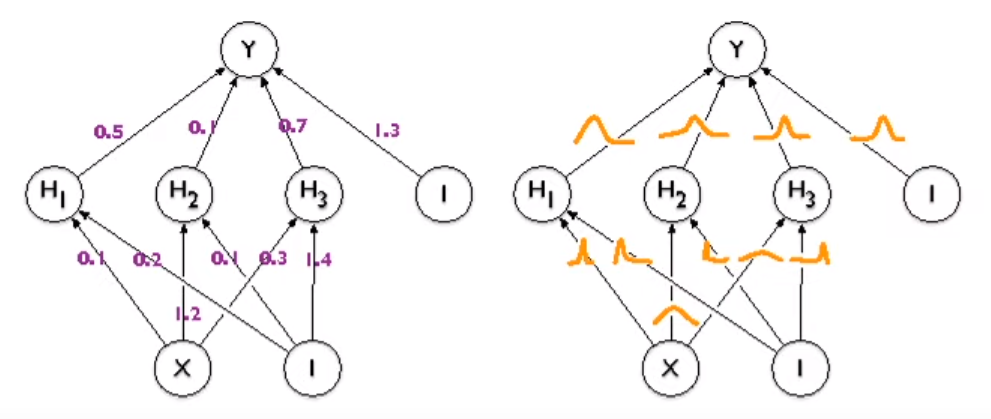
\includegraphics[width=.7\textwidth]{bayesian-neural-network.png}
		\caption{Normal neural network (left) and Bayesian neural network (right).}
	\end{figure}
	\begin{align}
		p(\theta | \mathcal{D}) & = \prod_{i} p(\theta_i | \mathcal{D}) && \text{common approximation}\\
		p(\theta_i | \mathcal{D}) & = \mathcal{N}(\mu_i, \sigma_i) && \text{common choice for each marginal \ac{prob}}
	\end{align}
	\item Bootstrap ensembles: train ensemble of models (\secref{sec:bagging}). Each model (usually $<10$ models) with \ac{param} $\theta_i$ is trained on a dataset $\mathcal{D}_i$, which is sampled with replacement from $\mathcal{D}$.
	\begin{align}
		&p(\theta | \mathcal{D}) \approx \frac{1}{N} \sum_{i} \delta(\theta_i) && \text{mixture of delta \ac{func}}\\
		&\int p(\textbf{s}_{t+1} | \textbf{s}_t, \textbf{a}_t, \theta) p(\theta|\mathcal{D}) d\theta \approx \frac{1}{N} \sum_i p(\textbf{s}_{t+1} | \textbf{s}_t, \textbf{a}_t, \theta)
	\end{align}
\end{itemize}

\section{Planning with Uncertainty}
As mentioned before, the model uncertainty is used in step 3 of the model-based \ac{RL} algorithm (\subsecref{subsec:uncertainty-aware-model}). The change is about the reward function that we use to do optimal control for action planning:
\begin{itemize}
	\item Before: $\displaystyle J(\textbf{a}_1,\dots, \textbf{a}_H) = \sum_{t=1}^{H} r(\textbf{s}_t, \textbf{a}_t)$ where $\textbf{s}_{t+1} = f(\textbf{s}_t, \textbf{a}_t) $
	\item Now: $\displaystyle J(\textbf{a}_1,\dots, \textbf{a}_H) = \frac{1}{N} \sum_{i=1}^{N} \sum_{t=1}^{H} r(\textbf{s}_{t,i}, \textbf{a}_{t,i})$ where $f(\textbf{s}_{t,i}, \textbf{a}_t) = \textbf{s}_{t+1, i}$ (deterministic case)
\end{itemize}

General procedure for candidate action sequence $\textbf{a}_1,\dots, \textbf{a}_H$:
\begin{enumerate}
	\item Sample $\theta \sim p(\theta | \mathcal{D})$
	\item At each time step $t$, sample $\textbf{s}_{t+1} \sim p(\textbf{s}_{t+1} | \textbf{s}_t, \textbf{a}_t, \theta) $
	\item Calculate $R = \sum_{t} r(\textbf{s}_t, \textbf{a}_t)$
	\item Repeat step $1\rightarrow3$ and accumulate the average reward
\end{enumerate}

\section{References}
\begin{itemize}
	\item \citeaustitle{deisenroth2011icml}
	\item \citeaustitle{chua2018deep}
	\item \citeaustitle{nagabandi2020deep}
	\item \citeaustitle{feinberg2018icml}
	\item \citeaustitle{buckman2018sample}
\end{itemize}
% !TeX spellcheck = en_US
\chapter{Model-based RL with Images}
\section{Latent Space Models}
In state space (latent-space) models, the inputs are given observations, not states.
\begin{align}
	& p(\textbf{o}_t | \textbf{s}_t) && \text{- observation model: high-dimensional, but not dynamic}\\
	& p(\textbf{s}_{t+1} | \textbf{s}_t, \textbf{a}_t) && \text{- dynamics model: low-dimensional, but dynamic}\\
	& p(r_t | \textbf{s}_t, \textbf{a}_t) && \text{- reward model}
\end{align}
\begin{center}
	\begin{tikzpicture}[roundnode/.style={circle, draw=black!60, very thick, minimum size=7mm}]
		\node[roundnode](s1){$\textbf{s}_1$};
		\node[roundnode](s2)[right=3cm of s1]{$\textbf{s}_2$};
		\node[roundnode](s3)[right=3cm of s2]{$\textbf{s}_3$};
		\node[roundnode](o1)[above left=1cm and 0.5cm of s1]{$\textbf{o}_1$};
		\node[roundnode](o2)[above left=1cm and 0.5cm of s2]{$\textbf{o}_2$};
		\node[roundnode](o3)[above left=1cm and 0.5cm of s3]{$\textbf{o}_3$};
		\node[roundnode](a1)[above right=1cm and 0.2cm of s1]{$\textbf{a}_1$};
		\node[roundnode](a2)[above right=1cm and 0.2cm of s2]{$\textbf{a}_2$};
		\node[roundnode](a3)[above right=1cm and 0.2cm of s3]{$\textbf{a}_3$};
		\node[roundnode](r1)[below right=.7cm and 0.5cm of s1]{$\textbf{r}_1$};
		\node[roundnode](r2)[below right=.7cm and 0.5cm of s2]{$\textbf{r}_2$};
		\node[roundnode](r3)[below right=.7cm and 0.5cm of s3]{$\textbf{r}_3$};
		\draw[-latex](s1.east) -- (s2.west);
		\draw[-latex](s2.east) -- (s3.west);
		\draw[-latex](a1.south east) -- (s2.west);
		\draw[-latex](a2.south east) -- (s3.west);
		\draw[-latex](s1.north west) -- (o1.south east);
		\draw[-latex](s2.north west) -- (o2.south east);
		\draw[-latex](s3.north west) -- (o3.south east);
		\draw[-latex](a1.south) -- (r1.north);
		\draw[-latex](a2.south) -- (r2.north);
		\draw[-latex](a3.south) -- (r3.north);
		\draw[-latex](s1.south east) -- (r1.north west);
		\draw[-latex](s2.south east) -- (r2.north west);
		\draw[-latex](s3.south east) -- (r3.north west);
	\end{tikzpicture}
\end{center}

With the above state space model, we now learn a different model:
\begin{itemize}
	\item Before: standard (fully observable) model
	\[ \underset{\phi}{\max} \frac{1}{N} \sum_{i=1}^N \sum_{t=1}^T \log p_\phi (\textbf{s}_{t+1, i} | \textbf{s}_{t, i}, \textbf{a}_{t,i}) \]
	\item Now: latent space model
	\[ \underset{\phi}{\max} \frac{1}{N} \sum_{i=1}^N \sum_{t=1}^T \mathbb{E}\left[ \log p_\phi (\textbf{s}_{t+1, i} | \textbf{s}_{t, i}, \textbf{a}_{t,i}) + \log p_\phi(\textbf{o}_{t,i}|\textbf{s}_{t, i}) \right] \]
	the expectation with regard to $(\textbf{s}_t, \textbf{s}_{t+1})\sim p(\textbf{s}_t, \textbf{s}_{t+1} | \textbf{o}_{1:T}, \textbf{a}_{1:T})$ \hlr{(very complicate)}
\end{itemize}

The above objective can be learn by the approximate posterior $q_\psi(\textbf{s}_t | \textbf{o}_{1:t}, \textbf{a}_{1:t})$ \hlr{"encoder"}. There are also other choices for approximate posterior, depending on each problem settings:
\begin{align*}
	&q_\psi(\textbf{s}_t, \textbf{s}_{t+1} | \textbf{o}_{1:T}, \textbf{a}_{1:T}) &&\text{full smoothing posterior} &&\begin{matrix*}[l]
		\color{Green}+ \text{most accurate}\\
		\color{red}- \text{most complicated (big \ac{RNN})}
	\end{matrix*}\\
	&\quad q_\psi(\textbf{s}_t | \textbf{o}_t) &&\text{single-step encoder} &&\begin{matrix*}[l]
		\color{Green}+ \text{simplest}\\
		\color{red}- \text{least accurate (\ac{CNN})}
	\end{matrix*}
\end{align*}
\begin{itemize}
	\item If the situation is more partially observed, you would want a more accurate approximation.
	\item If the state can be entirely guessed by one single current observation, then this single-step posterior is a good choice.
\end{itemize}

\section{Deterministic Single-Step Encoder}
Simple special case: $q(\textbf{s}_t, \textbf{o}_t)$ is \hlb{deterministic}
\begin{align}
	&q_\psi(\textbf{s}_t | \textbf{o}_t) = \delta(\textbf{s}_t = g_\psi(\textbf{o}_t)) \Rightarrow \textbf{s}_t = g_\psi(\textbf{o}_t) && \text{deterministic encoder}
\end{align}
$\Rightarrow$ The goal for model-based \ac{RL} with latent space is now:
\begin{equation}
	\underset{\phi, \psi}{\max} \frac{1}{N} \sum_{i=1}^N \sum_{t=1}^T \log p_\phi \left[g_\psi(\textbf{o}_{t+1, i}) | g_\psi(\textbf{o}_{t,i}), \textbf{a}_{t,i}\right] + \log p_\phi\left[ \textbf{o}_{t,i} | g_\psi(\textbf{o}_{t,i}) \right]
\end{equation}
\begin{align*}
	\underset{\phi, \psi}{\max} \frac{1}{N} \sum_{i=1}^N \sum_{t=1}^T &\log p_\phi \left[g_\psi(o_{t+1, i}) | g_\psi(o_{t,i}), a_{t,i}\right] + &\log p_\phi\left[ o_{t,i} | g_\psi(o_{t,i}) \right] + &&\log p_\phi \left[ r_{t, i} | g_\psi(o_{t,i}) \right]\\
	& \text{\hlr{\fontsize{11}{0}\selectfont latent space dynamics}} & \text{\hlr{\fontsize{11}{0}\selectfont image reconstruction}} && \text{\hlr{\fontsize{11}{0}\selectfont reward model}}
\end{align*}

\section{Model-based RL with Latent Space Model}
This is the model-based \ac{RL} with latent space model, assuming deterministic observation model:
\begin{enumerate}
	\item Run based policy $\pi_0(\textbf{a}_t|\textbf{o}_t)$ (\eg, random policy) to collect $\mathcal{D} = \{ (\textbf{o, a, o}')_i \}$
	\item \tikzmark{mbrllsm2}Learn $p_\phi(\textbf{s}_{t+1} | \textbf{s}_t, \textbf{a}_t), p_\phi(r_t, \textbf{s}_t), p(\textbf{o}_t | \textbf{s}_t), g_\psi(\textbf{o}_t)$
	\item \tikzmark{mbrllsm3}Plan through the model to choose actions (\eg, \ac{MCTS}, \ac{LQR}, random shooting)
	\item Execute the first planned action, observe result $\textbf{o}'$ (\ac{MPC})
	\item \tikzmark{mbrllsm5}Append resulting $(\textbf{o, a, o}')$ to $\mathcal{D}$
	\begin{tikzpicture}[overlay,remember picture]
		\draw[very thick, -latex]
		([xshift=-7mm,yshift=2mm]pic cs:mbrllsm5) --++ (-.5,0) |-
		([xshift=-7mm,yshift=1mm]pic cs:mbrllsm3);
		\draw[very thick, -latex]
		([xshift=-7mm,yshift=1mm]pic cs:mbrllsm5) --++ (-.7,0) |-
		([xshift=-7mm,yshift=1mm]pic cs:mbrllsm2);
		\node at ([xshift=-16mm,yshift=-2mm]pic cs:mbrllsm3) {\fontsize{10}{0}\selectfont \rotatebox{90}{every $N$ steps}};
	\end{tikzpicture}
\end{enumerate}

\section{Learning in Observation Space}
Im some situation, there are too many objects, thus, it's complicate to learn/build a compact state space. The better solution would be to directly learn $p(\textbf{o}_{t+1} | \textbf{o}_t, \textbf{a}_t)$ (taken in image $\rightarrow$ split out image).

References:
\begin{itemize}
	\item \citeaus{finn2017icra}. Deep visual foresight for planning robot motion.
	\item \citeaus{ebert2017self}. Self-Supervised Visual Planning with Temporal Skip Connections.
\end{itemize}

Gigantic model: \ac{RNN}. \todo{??}
% !TeX spellcheck = en_US
\chapter{Model-Based Policy Learning}
As mentioned before, model-based \ac{RL} v.1.5 algorithm (\secref{sec:modelbasedrl1.5}) is a \hlb{stochastic open-loop} algorithm. The agent does see the next state, but it doesn't able to reason about the fact that more information will be available and make use out it. It simply plans the whole action sequence at each time step and assumes that it has to commit to that complete action plan. This is, in most case, \hlr{sub-optimal}. This section describes the \hlb{closed-loop} case, implying the agent aware that it will be able to see the state feedback and act upon it. Thus, instead of a complete action plan, the output is now a policy $\pi(\textbf{a}_t | \textbf{s}_t)$.

\begin{itemize}
	\item Stochastic open-loop case:\quad $\left\{\begin{matrix*}[l]
		\displaystyle p_\theta(\textbf{s}_1, \dots, \textbf{s}_T | \textbf{a}_1, \dots, \textbf{a}_T) = p(\textbf{s}_1) \prod_{t=1}^T p(\textbf{s}_{t+1} | \textbf{s}_t, \textbf{a}_t)\\
		\displaystyle \textbf{a}_1, \dots, \textbf{a}_T = \underset{\textbf{a}_1, \dots, \textbf{a}_T}{\arg\max}\; \mathbb{E} \left[ \sum_t r(\textbf{s}_t, \textbf{a}_t) | \textbf{a}_1, \dots, \textbf{a}_T \right]
	\end{matrix*}\right.$
	\item Stochastic closed-loop case:\quad $\left\{ \begin{matrix*}[l]
		\displaystyle p(\textbf{s}_1, \textbf{a}_1, \dots, \textbf{s}_T, \textbf{a}_T) = p(\textbf{s}_1) \prod_{t=1}^T \pi(\textbf{a}_t | \textbf{s}_t) p(\textbf{s}_{t+1} | \textbf{s}_t, \textbf{a}_t)\\
		\displaystyle \pi = \underset{\pi}{\arg\max}\; \mathbb{E}_{\tau \sim p(\tau)} \left[ \sum_t r(\textbf{s}_t, \textbf{a}_t) \right]
	\end{matrix*} \right.$
\end{itemize}

For the above policy $\pi$, there are possibly different forms for it:
\begin{itemize}
	\item Neural net: \hlr{global policy}, which would tell us what to do regardless of the state the agent is in the whole state space.
	\item Time-varying linear $\textbf{K}_t \textbf{s}_t + \textbf{k}_t$: \hlr{local policy}, which would be simple but only sufficient around particular area of a known trajectory
\end{itemize}

\section{Model-based RL v.2.0}
\label{sec:model-based-rl-2.0}
\begin{center}
	\begin{tikzpicture}[recnode/.style={rectangle, draw=black!60, very thick, minimum size=7mm}]
		\node[recnode](a1){$\textbf{a}_t = \pi_\theta(\textbf{s}_t)$};
		\node[recnode](s1)[right=of a1]{$\textbf{s}_{t+1} = f(\textbf{s}_t, \textbf{a}_t)$};
		\node[recnode](a2)[right=of s1]{$\textbf{a}_t = \pi_\theta(\textbf{s}_t)$};
		\node[recnode](s2)[right=of a2]{$\textbf{s}_{t+1} = f(\textbf{s}_t, \textbf{a}_t)$};
		\node[recnode](r1)[above=of a1]{$r(\textbf{s}_t, \textbf{a}_t)$};
		\node[recnode](r2)[above=of a2]{$r(\textbf{s}_t, \textbf{a}_t)$};
		\draw[thick, -latex, transform canvas={yshift=-2.5pt}](a1.east) -- (s1.west);
		\draw[red, thick, latex-, transform canvas={yshift= 2.5pt}](a1.east) -- (s1.west) node[midway, above=.2cm]{backprop};
		\draw[thick, -latex, transform canvas={yshift=-2.5pt}](a2.east) -- (s2.west);
		\draw[red, thick, latex-, transform canvas={yshift= 2.5pt}](a2.east) -- (s2.west) node[midway, above=.2cm]{backprop};
		\draw[thick, -latex, transform canvas={yshift=-2.5pt}](s1.east) -- (a2.west);
		\draw[red, thick, latex-, transform canvas={yshift= 2.5pt}](s1.east) -- (a2.west) node[midway, above=.2cm]{backprop};
		\draw[red, thick, -latex, transform canvas={xshift= 4.5pt}](r1.south) -- (a1.north);
		\draw[thick, latex-, transform canvas={xshift=-4.5pt}](r1.south) -- (a1.north);
		\draw[red, thick, -latex, transform canvas={xshift= 4.5pt}](r2.south) -- (a2.north);
		\draw[thick, latex-, transform canvas={xshift=-4.5pt}](r2.south) -- (a2.north);
	\end{tikzpicture}
\end{center}
\begin{enumerate}
	\item Run based policy $\pi_0(\textbf{a}_t, \textbf{s}_t)$ to collect $\mathcal{D} = \{ (\textbf{s, a, s'})_i \}$
	\item \tikzmark{mbrlv22}Learn dynamic model $f(\textbf{s,a})$ to minimize $\sum_{i} || f(\textbf{s}_{i}, \textbf{a}_{i}) - \textbf{s}_{i}' ||^2$
	\item Back-propagate through $f(\textbf{s,a})$ into the policy to optimize $\pi_\theta(\textbf{a}_t, \textbf{s}_t)$
	\item \tikzmark{mbrlv24}Run $\pi_\theta(\textbf{a}_t, \textbf{s}_t)$, appending the tuples $(\textbf{s, a, s'})$ to $\mathcal{D}$
	\begin{tikzpicture}[overlay,remember picture]
		\draw[very thick, -latex]
		([xshift=-7mm,yshift=1mm]pic cs:mbrlv24) --++ (-.5,0) |-
		([xshift=-7mm,yshift=1mm]pic cs:mbrlv22);
	\end{tikzpicture}
\end{enumerate}

\hlb{Problem:}
\begin{itemize}
	\item Similar parameter sensitivity problems as shooting methods\\
	The first action is way more important the the later ones.
	\item Similar problems to training long \ac{RNN}s with \ac{BPTT}\\
	Vanishing and exploding \ gradients
\end{itemize}

$\Rightarrow$ \hlb{Solutions:}
\begin{itemize}
	\item Use derivative-free ("model-free") planning algorithms with the model used to generate synthetic samples\\
	\Eg: Policy gradients has high variance, which can be reduced with lots of data, which can be generated by learned model
	\item Use simpler policies than neural nets
	\begin{itemize}
		\item \ac{LQR} with learned models (\ac{LQR}-\ac{FLM})
		\item Train \textbf{local} policies to solve simple tasks
		\item Combine them into \textbf{global} policies via supervised learning
	\end{itemize}
\end{itemize}

\section{Model-Free Learning With a Model}
This is one of the solutions for Model-based \ac{RL} v.2.0 (\secref{sec:model-based-rl-2.0}): use the learned model to generate synthetic data for "model-free" \ac{RL} algorithms, \eg, policy gradient. \cite{parmas2018icml}

\hlb{"Classic" Dyna} \cite{sutton1990integrated}: online Q-learning \ac{algor} that performs model-free \ac{RL} with a model
\begin{enumerate}
	\item Given state $s$, pick action $a$ using exploration policy
	\item Observe $s'$ and $r$, to get transition $(s, a, s', r)$
	\item Update model $\widehat{p}(s'|s,a)$ and $\widehat{r}(s,a)$ using $(s,a,s')$
	\item Q-update: $Q(s,a) \leftarrow Q(s,a) + \alpha \mathbb{E}_{s', r} [r + \underset{a'}{\max} Q(s', a') - Q(s, a) ]$
	\item Repeat $K$ times:\\
	6. \tikzmark{dyna5}Sample $(s,a) \sim \mathcal{B}$ from buffer of past states and actions\\
	7. \tikzmark{dyna6}Q-update: $Q(s,a) \leftarrow Q(s,a) + \alpha \mathbb{E}_{s', r} [r + \underset{a'}{\max} Q(s', a') - Q(s, a) ]$
	\begin{tikzpicture}[overlay,remember picture]
		\draw[very thick, -latex]
		([xshift=-7mm,yshift=1mm]pic cs:dyna6) --++ (-.5,0) |-
		([xshift=-7mm,yshift=1mm]pic cs:dyna5);
	\end{tikzpicture}
\end{enumerate}

\hlb{General "Dyna-style" model-based \ac{RL}:}
\begin{enumerate}
	\item Collect some data, consisting of transitions $(\textbf{s, a, s'}, r)$ \hlr{(1-million steps)}
	\item Learn model $\widehat{p}(s'|s,a)$ (and optionally, $\widehat{r}(s,a)$)
	\item Repeat $K$ times:\\
	4. Sample $s \sim \mathcal{B}$ from buffer\\
	5. Choose action $a$ (from $\mathcal{B}$, from $\pi$, or random)\\
	6. Simulate $s' \sim\widehat{p}(s'|s,a)$ (and $r = \widehat{r}(s,a)$)\\
	7. Train on $(s, a, s', r)$ with model-free \ac{RL}\\
	8. (optional) Take $N$ more model-based steps
\end{enumerate}
The above approach is:
\[\begin{matrix*}[l]
	\color{Green}+ \text{only requires short (as few as one step) rollouts from model}\\
	\color{Green}+ \text{still sees diverse states}
\end{matrix*}\]
\hlb{Problem:} if your model is inaccurate (which always is), the longer we roll-out the model, the more these errors compound. This leads to distribution shift, either in the model or the policy. This is also why this is suited for mostly short rollouts of the model.
$\Rightarrow$ Not very nice for Policy Gradients, but is okay for value-based approaches, actor-critic, \etc.

\hlb{Note:}
\begin{itemize}
	\item In Classic Dyna, step 5 is to choose action from buffer
	\item This general procedure is the basis for:
	\begin{itemize}
		\item \ac{MBA} \cite{gu2016continuous}
		\item \ac{MVE} \cite{feinberg2018model}
		\item \ac{MBPO} \cite{janner2019trust}
	\end{itemize}
\end{itemize}

\section{Local Models}
This is the second solution for model-based \ac{RL} v.2.0 (\secref{sec:model-based-rl-2.0}): instead of using neural network, we use simple policies, which is time-varying linear controller, \ie, \ac{LQR}-\ac{FLM}.

In order to use \ac{LQR} (\secref{sec:lqr}), we need $\displaystyle\frac{df}{d\textbf{x}_t}, \frac{df}{d\textbf{u}_t}, \frac{dc}{d\textbf{x}_t}, \frac{dc}{d\textbf{u}_t}$. In which, knowing the model would give us $\displaystyle\frac{df}{d\textbf{x}_t}, \frac{df}{d\textbf{u}_t}$.\\
$\Rightarrow$ \hlb{Idea:} fit $\displaystyle\frac{df}{d\textbf{x}_t}$ and $\displaystyle\frac{df}{d\textbf{u}_t}$ around \hlb{current trajectory / policy}

If continuous system sufficiently smooth and initial state distribution quite tight $\Rightarrow$ do linearization regression at every time step

\hlb{\ac{LQR}-\ac{FLM} Algorithm:}
\begin{enumerate}
	\item \tikzmark{lqr-flm1}Run $p(\textbf{u}_t | \textbf{x}_t)$ on robot, collect $\mathcal{D} = \{\tau_i\}$
	\item Fit dynamics $p(\textbf{x}_{t+1} | \textbf{x}_t, \textbf{u}_t)$
	\begin{align*}
		&p(\textbf{x}_{t+1} | \textbf{x}_t, \textbf{u}_t) = \mathcal{N}(f(\textbf{x}_t, \textbf{u}_t), \Sigma)\\
		&f(\textbf{x}_t, \textbf{u}_t) \approx \textbf{A}_t \textbf{x}_t + \textbf{B}_t \textbf{u}_t\\
		&\textbf{A}_t = \frac{df}{d\textbf{x}_t} \quad \textbf{B}_t = \frac{df}{d\textbf{u}_t}
	\end{align*}
	\item \tikzmark{lqr-flm3}Improve controller $p(\textbf{u}_t | \textbf{x}_t)$ (\ac{LQR})
	\begin{tikzpicture}[overlay,remember picture]
		\draw[very thick, -latex]
		([xshift=-7mm,yshift=1mm]pic cs:lqr-flm3) --++ (-.5,0) |-
		([xshift=-7mm,yshift=1mm]pic cs:lqr-flm1);
	\end{tikzpicture}
\end{enumerate}

\hlb{Which controller to run?} $p(\textbf{u}_t | \textbf{x}_t)$
\begin{itemize}
	\item Version 0.5: $p(\textbf{u}_t | \textbf{x}_t) = \delta(\textbf{u}_t = \widehat{\textbf{u}}_t)$ doesn't correct deviations or drift
	\item Version 1.0: $p(\textbf{u}_t | \textbf{x}_t) = \delta \textbf{u}_t = \textbf{K}_t (\textbf{x}_t - \widehat{\textbf{x}}_t) + \textbf{k}_t + \widehat{\textbf{u}}_t$\\
	Better, but a little too good. When fitting the dynamics, we need data to be a little bit cluster, but not too much. \hlr{Still need to be varied, for exploration and fitting.}
	\item Version 2.0: $p(\textbf{u}_t | \textbf{x}_t) = \mathcal{N}(\textbf{K}_t (\textbf{x}_t - \widehat{\textbf{x}}_t) + \textbf{k}_t + \widehat{\textbf{u}}_t, \Sigma_t)$\\
	Set $\Sigma_t = \textbf{Q}_{\textbf{u}_t, \textbf{u}_t}^{-1}$
\end{itemize}

\hlb{How to fit the dynamics?} $p(x_{t+1} | x_t, u_t)$ given $\{ (\textbf{x}_t, \textbf{u}_t, \textbf{x}_{t+1})_i \}$
\begin{itemize}
	\item Version 1.0: At each time step using linear regression
	\[ p(\textbf{x}_{t+1} | \textbf{x}_t, \textbf{u}_t) = \mathcal{N}(\textbf{A}_t \textbf{x}_t + \textbf{B}_t \textbf{u}_t + \textbf{c}, \textbf{N}_t); \quad \textbf{A}_t \approx \frac{df}{d\textbf{x}_t}; \textbf{B}_t \approx \frac{df}{d\textbf{u}_t} \]
	\hlb{Problems:} linear regression requires number of samples that scale with dimensional states
	\item Version 2.0: fit using Bayesian linear regression\\
	Use your favorite global model as prior\\
	$\Rightarrow$ Can get away with fewer samples
\end{itemize}

\hlb{How to stay close to old controller?}\\
We want to stay close around local region of trajectories where we have linearize to approximation\\
$\Rightarrow$ Keep \ac{KL} divergence small (between old and new trajectories) \cite{levine2014learning}
\begin{align}
	&p(\textbf{u}_t | \textbf{x}_t) = \mathcal{N}(\textbf{K}_t (\textbf{x}_t - \widehat{\textbf{x}}_t) + \textbf{k}_t + \widehat{\textbf{u}}_t, \Sigma_t) && \text{the controller}\\
	&p(\tau) = p(\textbf{x}_1) \prod_{t=1}^T p(\textbf{u}_t | \textbf{x}_t) p(\textbf{x}_{t+1} | \textbf{x}_t, \textbf{u}_t) && \text{the resulting trajectory}\\
	& D_{KL}(p(\tau) || \bar{p}(\tau)) \leq \epsilon && \text{constraint on \ac{KL} divergence}
\end{align}

\section{Guided Policy Search}
This is the extension of local policies to global policies. However, the idea behind this, which is similar to distillation of ensemble (Sec. 5.8, \href{AI_notes.pdf}{AI notes}), is also important in other settings.

Given many local policies, we take the data from these local policies and treat them as demonstrations of expert and combine them into a global policy. The global policy can now be represented by a neural net and learned by supervised learning from these local data.

\hlb{Guided Policy Search Algorithm:} \cite{levine2016end}
\begin{enumerate}
	\item \tikzmark{gps1}Optimize each local policy $\pi_{LQR, i}(\textbf{u}_t | \textbf{x}_t)$ on initial state $\textbf{x}_{0, i}, \text{ \ac{wrt} } \widetilde{c}_{k,i}(\textbf{x}_t, \textbf{u}_t)$
	\item Use samples from step (1) to train $\pi_{\theta}(\textbf{u}_t|\textbf{x}_t)$ to mimic all $\pi_{LQR, i}(\textbf{u}_t | \textbf{x}_t)$
	\item \tikzmark{gps3}Update cost function $\widetilde{c}_{k+1,i}(\textbf{x}_t, \textbf{u}_t) = c(\textbf{x}_t, \textbf{u}_t) + \lambda_{k+1, i} \log\pi_{\theta}(\textbf{u}_t | \textbf{x}_t)$
	\begin{tikzpicture}[overlay,remember picture]
		\draw[very thick, -latex]
		([xshift=-7mm,yshift=1mm]pic cs:gps3) --++ (-.5,0) |-
		([xshift=-7mm,yshift=1mm]pic cs:gps1);
	\end{tikzpicture}
\end{enumerate}
in which, $i$ indexes the initial state and the local solution, $k$ the iteration, $\widetilde{c}_{k,i}(\textbf{x}_t, \textbf{u}_t)$ is the modified cost, including the task reward, and the \ac{KL} between $\pi_{LQR, i}$ and $\pi_{\theta}PP$

\begin{figure}[hbt!]
	\centering
	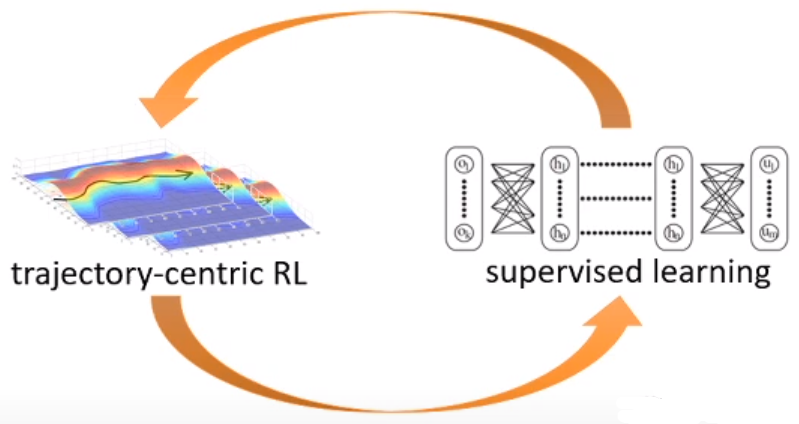
\includegraphics[width=.57\textwidth]{guided-policy-search.png}
	\caption{Guided policy search: algorithm sketch (\href{https://www.youtube.com/watch?v=DszxsbAl8Eo&list=PL_iWQOsE6TfURIIhCrlt-wj9ByIVpbfGc&index=55}{src}).}
\end{figure}

\hlb{Divide and Conquer \ac{RL} algorithm:}
\begin{enumerate}
	\item \tikzmark{dac1}Optimize each local policy $\pi_{\theta, i}(\textbf{u}_t | \textbf{x}_t)$ on initial state $\textbf{x}_{0, i}, \text{ \ac{wrt} } \widetilde{r}_{k,i}(\textbf{x}_t, \textbf{u}_t)$
	\item Use samples from step (1) to train $\pi_{\theta}(\textbf{u}_t|\textbf{x}_t)$ to mimic all $\pi_{\theta, i}(\textbf{u}_t | \textbf{x}_t)$
	\item \tikzmark{dac3}Update cost function $\widetilde{r}_{k+1,i}(\textbf{x}_t, \textbf{u}_t) = r(\textbf{x}_t, \textbf{u}_t) + \lambda_{k+1, i} \log\pi_{\theta}(\textbf{u}_t | \textbf{x}_t)$
	\begin{tikzpicture}[overlay,remember picture]
		\draw[very thick, -latex]
		([xshift=-7mm,yshift=1mm]pic cs:dac3) --++ (-.5,0) |-
		([xshift=-7mm,yshift=1mm]pic cs:dac1);
	\end{tikzpicture}
\end{enumerate}

\section{References}
\begin{itemize}
	\item \citeausm{levine2016end}. End-to-end training of deep visuomotor policies.
	\item \citeausm{rusu2015policy}. Policy distillation.
	\item \citeausm{parisotto2015actor}. Actor-mimic: Deep multitask and transfer reinforcement learning.
	\item \citeausm{ghosh2017divide}. Divide-and-conquer reinforcement learning.
	\item \citeausm{teh2017distral}. Distral: Robust multitask reinforcement learning.
\end{itemize}
% !TeX spellcheck = en_US
\chapter{Exploration}

\section{Overview}
In the setting of delayed reward, not knowing which actions would give more reward, we would want the agent to \textit{explore}. The concerns are:
\begin{itemize}
	\item How can an agent discover high-reward strategies that require a temporally extended sequence of complex behaviors that, individually, are not rewarding?
	\item How can an agent decide whether to attempt new behaviors (to discover ones with higher reward) or continue to do the best things it knows so far?
\end{itemize}
This poses a exploration and exploitation dilemma:
\begin{itemize}
	\item \textit{Exploration}: doing things you haven't done before, in the hopes of getting even higher reward
	\item \textit{Exploitation}: doing what you know will yield the highest reward
\end{itemize}

\subsection{Regret}
\label{sec:regret}
Exploration can be viewed as a \ac{POMDP}. Solving the \ac{POMDP} to know the exact underlying distribution is overkill. We instead want a simpler strategy that is not too bad from the optimal ones. The \textit{regret} is the metric to measure how good or bad an exploration strategy.

\hlb{Definition:} \textit{Regret} is the reward difference from optimal policy at time step $T$:
\begin{align*}
	&\underbrace{Reg(T)}_{\textstyle \text{regret at $T$}} = &&T. \underbrace{\mathbb{E}[r(a^*)]}_{\textstyle \text{expected reward of the best action}} && - \underbrace{\sum_{t=1}^T r(a_t)}_{\textstyle \text{the actual sum of reward}}
\end{align*}

\hlb{Example:} Consider the following multi-armed bandit problem:\\
A professor moves to a small town for work. He will stay there for 300 days. Each day, he will eat at one of three restaurants in the town. Eating at each restaurant has a different happiness distribution. Let say, the happiness distributions of each restaurant are as follows:
\begin{itemize}
	\item Restaurant 1: $\mu=10, \sigma=5$
	\item Restaurant 2: $\mu=8, \sigma=8$
	\item Restaurant 3: $\mu=5, \sigma=25$
\end{itemize}
\textbf{Not knowing the true happiness distribution, which strategy should the professor follow to maximize the expected happiness score?}

The regrets for some exploration strategies:
\begin{itemize}
	\item Optimal reward: Knowing the true distribution, the optimal action is to always go to restaurant 1.
	\[ \mathbb{E}[r] = 300 \times 10 = 3000\]
	\item Explore only: the professor spends 100 days at each restaurant.
	\begin{align*}
		\mathbb{E}[r] &= 100 \times 10 + 100 \times 8 + 100 \times 5 = 2300\\
		\Rightarrow \rho &= 3000 - 2300 = 700 \qquad \text{(regret)}
	\end{align*}
	\item Exploit only: visit each restaurant once, then stick with the one with the highest value.\\
	Assume the receive reward after 3 days are: $r_1 = 7, r_2 = 8, r_3 = 5$. After that, the expected reward would be:
	\[ \mathbb{E}[r] = 7 + 8 + 5 + (300 - 3) \times 8 = 2396 \]
	However, this is not the actual expected reward for the exploit only strategy.
	\[\rho = 3000 - 2670 = 330\]
	\item Zero regret strategy: As time goes on $T\rightarrow \infty$, the regret will approach to 0 $\rho \rightarrow0$
\end{itemize}

\subsection{Optimality}
\textit{Optimality}: An exploration strategy is \textit{optimal} when we compared the regret \ac{vs} the Bayes-optimal strategy. \todo{}

\todo{Optimal exploration in small \ac{MDP}s}

\subsection{Tractability}
\begin{itemize}
	\item With \textit{theoretically tractable} exploration strategy, we can quantify or understand whether the given exploration strategy is optimal or sub-optimal
	\item With \textit{theoretically intractable} exploration strategy, we cannot make the above estimate exactly.
\end{itemize}

\begin{center}
	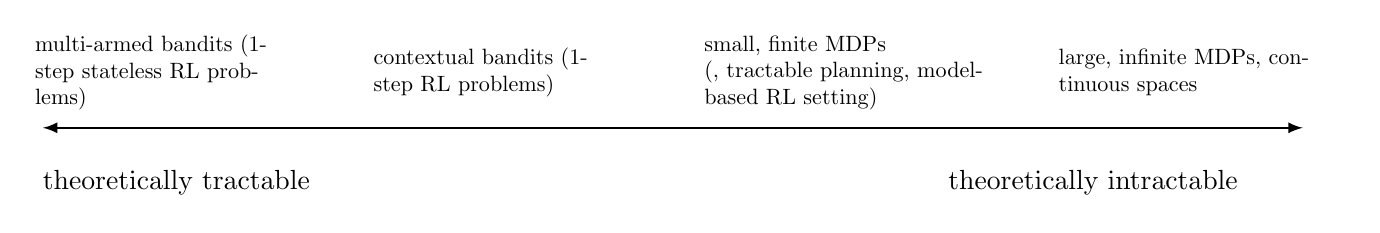
\begin{tikzpicture}
		\draw[thick,latex-latex] (-8,0) -- (8,0);
		\node[text width=5cm] at (-5.5,-.7) {theoretically tractable};
		\node[text width=5cm] at (6,-.7) {theoretically intractable};			
		\node[scale=0.8, text width=4cm] at (-6.5,.7) {multi-armed bandits (1-step stateless \ac{RL} problems)};
		\node[scale=0.8, text width=4cm] at (-2.2,.7) {contextual bandits (1-step \ac{RL} problems)};
		\node[scale=0.8, text width=4.5cm] at (2.2,.7) {small, finite \ac{MDP}s\newline (\eg, tractable planning, model-based \ac{RL} setting)};
		\node[scale=0.8, text width=4cm] at (6.5,.7) {large, infinite \ac{MDP}s, continuous spaces};
	\end{tikzpicture}
\end{center}

\begin{itemize}
	\item multi-armed bandits: can formalize exploration as \ac{POMDP} identification
	\item contextual bandits: policy learning is trivial even with \ac{POMDP}
	\item small, finite \ac{MDP}s: can frame as Bayesian model identification, reason explicitly about value of information
	\item large or infinite \ac{MDP}s: optimal methods don’t work, but can take inspiration from optimal methods in smaller settings
\end{itemize}

\section{Bandits Problems}
\subsection{One-Armed Bandit}
One armed bandit is the slot machine. It can be represent as a \ac{MDP} with one single action. The \ac{prob} distribution of the reward is unknown.
\begin{align}
	&\mathcal{A} = \{\text{pull arm}\}\\
	&r(\text{pull arm}) = ?
\end{align}

\begin{figure}[hbt!]
	\centering
	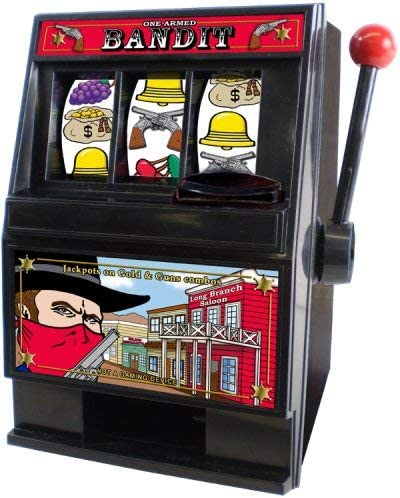
\includegraphics[width=.2\textwidth]{one-armed-bandit.png}
	\caption{One-armed bandit (\href{https://www.amazon.com/Armed-Bandit-Slot-Machine-Bank/dp/B001KYV9DW}{src}).}
\end{figure}

\subsection{Multi-Armed Bandit}
Multi armed bandit is a bank of multiple one-armed bandit slot machines. This problem is a 1-step stateless \ac{MDP}. Different machines have different reward distributions, which are unknown, but can be learned by trials.
\begin{align}
	&\mathcal{A} = \{\text{pull}_1, \text{pull}_2, \dots, \text{pull}_n\}\\
	&r(a_n) = ?\\
	&\text{assume } r(a_n) \sim p(r|a_n)
\end{align}

We can define the bandits as a \ac{POMDP} with the state as \ac{param} that represents the reward models. Solving the \ac{POMDP} leads to the optimal exploration strategy.
\[ \textbf{s} = [\theta_1, \dots, \theta_n]\]
But the belief state of $\theta$ is large, thus, doing this is overkill. We can do well with simpler strategies.

\subsection{Contextual Bandits}
\begin{itemize}
	\item the reward distribution depends on some external measurable variable.
	\item bandits with state, essentially 1-step \ac{MDP}
	\item \todo{}
\end{itemize}

\subsection{Bandit Variants}
\begin{itemize}
	\item Infinite Arms: there are more slot machines.
	\item Variable Arms: the reward distribution varies for each slot machine.
	\item Combinatorial Bandits: the agent has to pull more than one arm at once.
	\item Dueling Bandits: agent always pulls two arms, is never told about the reward, \dots
	\item Continuous Bandits: agent has to choose interval value, like the force to the arm.
	\item Adversarial Arms: the agent plays against an opponent. Thus if the agent uses the same strategy, the opponent will adapt, and the Q-value of that action will change over time. \Eg: chess, tic-tac-toe.
	\item Strategic Arms
	\item and more!
\end{itemize}

\subsection{Gradient Bandits}
\todo{}

\subsection{Applications}
There are various applications in:
\begin{itemize}
	\item Ad serving: arms - possible ads, reward - a click
	\item Website optimization: arms: possible website options, reward - user engagement
	\item Clinical trials: arms: possible medications, reward - health outcomes
\end{itemize}

\section{Exploration Strategies for Bandits Problem}
\subsection{$\epsilon$-first}
\todo{}

\subsection{$\epsilon$-greedy}
\todo{formula}

With the example in \secref{sec:regret}, assuming $\epsilon = 10\%$, the professor spend 10\% of the days (30 days) to try non-optimal restaurants, and the rest to exploit the current belief about the best restaurant.
\[\rho \approx 100\]

\subsection{Optimistic Exploration}
\label{subsec:bandits-optimistic-exploration}
The high-level idea is to try each arm until you are sure it's not great.
\begin{itemize}
	\item Keep track of average reward $\widehat{\mu}_a$ for each action $a$
	\item Optimistic estimate: $a = \underset{a}{\arg\max} [\widehat{\mu}_a + C \sigma_a]$.\\
	Choose the action with either current high average reward, or with high covariance $\sigma_a$
\end{itemize}

\ac{UCB}:
\[ A_t = \underset{a}{\arg\max} \left[ Q_t(a) + c\sqrt{\frac{\ln t}{N_t(a)}}\; \right], \qquad\begin{cases}
	Q_t(a) - \text{current reward belief}\\
	N_t(a) - \text{\ac{no} times taking action $a$}\\
	t - \text{current \ac{no} time step}
\end{cases} \]

\ac{UCB}-1 use Chernoff - Hoeffding Inequality, with $Reg(T) = \mathcal{O}(\log T)$:
\[ C_j(t) = \sqrt{\frac{\log(n)}{T_j(t	)}} \]
\[ a = \underset{a}{\arg\max} \left[\widehat{\mu}_a + \sqrt{\frac{2\ln T}{N(a)}}\;\right] \]
\note
\begin{itemize}
	\item lots of other functions work as well, as long as they decrease with $N(a)$
	\item \ac{UCB} is more difficult than $\epsilon$-greedy to extend beyond bandits to more general \ac{RL} problems (nonstationary problems, large state spaces)
\end{itemize}

\subsection{Probability Matching / Posterior Sampling}
\label{subsec:bandits-posterior-sampling}
Optimistic strategy doesn't try to model the uncertainty. It is model-free approach, simply keeps the average rewards and the number of times an action is taken. For the multi bandits problem, assuming some reward model $r(a_i)\sim p_{\theta_i}(r_i)$, we could instead keep a belief $\widehat{p}(\theta_1, \dots, \theta_n)$ over the \ac{param} and solve the \ac{POMDP} with $\textbf{s} = [\theta_1, \dots, \theta_n]$.

\hlb{Idea:} Thompson sampling \cite{chapelle2011empirical}
\begin{enumerate}
	\item \tikzmark{pm1}Sample $\theta_1, \dots, \theta_n \sim \widehat{p}(\theta_1, \dots, \theta_n)$
	\item Pretend the model $\theta_1, \dots, \theta_n$ is correct
	\item Take the optimal action $a = \underset{a}{\arg\max} \mathbb{E}_{\theta_a} [r(a)]$
	\item \tikzmark{pm4}Update the model
	\begin{tikzpicture}[overlay,remember picture]
		\draw[very thick, -latex]
		([xshift=-7mm,yshift=1mm]pic cs:pm4) --++ (-.5,0) |-
		([xshift=-7mm,yshift=1mm]pic cs:pm1);
	\end{tikzpicture}
\end{enumerate}

\begin{itemize}
	\item Harder to analyze theoretically
	\item Can work very well empirically
\end{itemize}

\subsection{Information Gain}
\label{subsec:bandits-information-gain}
This method is even more explicitly model-based.

\hlb{Bayesian experimental design:} aim to determine some unknown latent variable $z$ but can only take actions to learn about it.
\begin{align*}
	&\mathcal{H}(\widehat{p}(z)) &&-\text{the current entropy of $z$ estimate}\\
	&\mathcal{H}(\widehat{p}(z)|y) &&-\text{the entropy of $z$ estimate after observation $y$}\\
	&IG(z,y) = \mathbb{E}_y \big[\mathcal{H}(\widehat{p}(z)) - \mathcal{H}(\widehat{p}(z)|y)\big] &&-\text{the \textit{information gain} about $z$ after $y$}\\
	&IG(z,y | a) = \mathbb{E}_y \big[\mathcal{H}(\widehat{p}(z)) - \mathcal{H}(\widehat{p}(z)|y) | a\big] &&-\text{usually condition on action $a$}
\end{align*}

\begin{itemize}
	\item \eg, $y$ might be optimal action $a^*$ or the reward $r(a)$)
	\item We want to take actions and receive $y$ such that we get high \ac{IG} about $z$
\end{itemize}

\Eg, bandit \ac{algor} \cite{russo2014learning}:
\begin{align}
	& y = r_a && -\text{reward for action $a$}\\
	& z = \theta_a && -\text{\ac{param} of model $p(r_a)$} \\
	& g(a) = IG(\theta_a, r_a | a) && -\text{information gain of } a\\
	& \Delta(a) = \mathbb{E}[ r(a^*) - r(a) ] && -\text{expected suboptimality of } a\\
	\Rightarrow & a = \underset{a}{\arg\min} \frac{\Delta(a)^2}{g(a)}
\end{align}
the high-level idea is to take the least suboptimal action that give us more information.

\todo{Bayesian Model-based \ac{RL}}\\
\todo{\ac{PAC} exploration}

\section{Exploration Strategies in RL}
\subsection{Information Theoretic Quantities in RL}
\begin{align*}
	&\pi(\textbf{s}) = p_\pi(\textbf{s}) &&-\text{state \textit{marginal} distribution of policy $\pi$}\\
	&\mathcal{H}(\pi(\textbf{s})) &&-\text{state \textit{marginal} entropy of policy $\pi$}\\
	&\mathcal{I}(\textbf{x;y}) = D_{KL} \big( p(\textbf{x,y}) || p(\textbf{x}) p(\textbf{y}) \big) &&-\text{mutual information (\href{math_notes.pdf}{math notes})}\\
	&\mathcal{I}(\textbf{s}_{t+1};\textbf{a}_t) = \mathcal{H}(\textbf{s}_{t+1}) - \mathcal{H}(\textbf{s}_{t+1} | \textbf{a}_t) &&-\text{\textit{empowerment}}	
\end{align*}

\hlb{Intuition:} we want a large empowerment because: A large entropy $\mathcal{H} (\textbf{s}_{t+1})$ implies that there are many possible next states. A small entropy $\mathcal{H}(\textbf{s}_{t+1} | \textbf{a}_t)$ implies that given current action, it's easy to determine where the state will landed.

\subsection{Optimistic Exploration in Deep RL}
For bandits problem, \ac{UCB} chooses the action with $a = \underset{a}{\arg\max} \widehat{\mu}_a + \sqrt{\frac{2\ln T}{N(a)}}$ (\subsecref{subsec:bandits-optimistic-exploration}). The term $\sqrt{\frac{2\ln T}{N(a)}}$ can be considered as "exploration bonus". Lots of functions work, as long as they decrease with the count $N(a)$.

For \ac{MDP}s, we use similar state counts $N(\textbf{s, a})$ or $N(\textbf{s})$ to add \textit{exploration bonus}:
\begin{align}
	&r^+(\textbf{s,a}) = r(\textbf{s,a}) + \mathcal{B}(N(s)) && -\text{updated reward function}\\
	&\mathcal{B}(N(s)) && -\text{bonus that decreases with $N(\textbf{s})$}
\end{align}
\[\begin{matrix*}[l]
	\color{Green}+ \text{simple addition to any model-free \ac{RL} \ac{algor}}\\
	\color{red}- \text{need to tune bonus weight}
\end{matrix*}\]

In most settings of continuous state and action space, the agent might not literally visit the exact state again.\\
$\Rightarrow$ \hlb{Pseudo-counts:} to count similar states $\hat{N}(\textbf{s})$ or $\hat{N}(\textbf{s,a})$ \cite{bellemare2016unifying}
\begin{enumerate}
	\item \tikzmark{pc1}fit model $p_\theta(\textbf{s})$ to all states $\mathcal{D}$ seen so far
	\item take a step $i$ and observe $\textbf{s}_i$
	\item fit new model $p_{\theta'}(\textbf{s})$ to $\mathcal{D} \bigcup \textbf{s}_i$
	\item use $p_{\theta}(\textbf{s}_i)$ and $p_{\theta'}(\textbf{s}_i)$ to estimate $\hat{N}(\textbf{s})$
	\item \tikzmark{pc5}set $r_i^+ = r_i + \mathcal{B}(\hat{N}(\textbf{s}))$
	\begin{tikzpicture}[overlay,remember picture]
		\draw[very thick, -latex]
		([xshift=-7mm,yshift=1mm]pic cs:pc5) --++ (-.5,0) |-
		([xshift=-7mm,yshift=1mm]pic cs:pc1);
	\end{tikzpicture}
\end{enumerate}
\[ \hat{N}(\textbf{s}_i) = \hat{n} p_\theta(\textbf{s}_i), \qquad \hat{n} = \frac{1 - p_{\theta'}(\textbf{s}_i)}{p_{\theta'}(\textbf{s}_i) - p_\theta(\textbf{s}_i)} p_\theta(\textbf{s}_i) \]

\hlb{Types of exploration bonus:}
\begin{align}
	&- \text{\ac{UCB}:} &&\mathcal{B}(N(\textbf{s})) = \sqrt{\frac{2\ln n}{N(\textbf{s})}}\\
	&- \text{MBIE-EB: \cite{strehl2008analysis, bellemare2016unifying}} &&\mathcal{B}(N(\textbf{s})) = \sqrt{\frac{1}{N(\textbf{s})}}\\
	&- \text{BEB: \cite{kolter2009near}} &&\mathcal{B}(N(\textbf{s})) = \frac{1}{N(\textbf{s})}
\end{align}

\hlb{Kind of model:} $p_\theta(\textbf{s})$ need to output densities, but not necessarily produce great samples
\begin{itemize}
	\item CTS model \cite{bellemare2016unifying}
	\item stochastic neural networks
	\item compression length
	\item EX2
\end{itemize}

There are similar count style approaches:
\begin{itemize}
	\item Counting with hashes: counts states but in different space \cite{tang2017exploration}.
	\item Implicit density modeling with exemplar models: Use a classifier to classify whether a state is \textbf{novel} or not. \cite{fu2017ex2}
	\item Heuristics estimation of counts via errors: Given buffer $\mathcal{D} = \{(\textbf{s}_i, \textbf{a}_i)\}$
	\begin{itemize}
		\item Fit $\hat{f}_\theta(\textbf{s,a})$ to \textbf{target} function $f^*(\textbf{s,a})$
		\item Use $\mathcal{E}(\textbf{s,a}) = \left|\left| \hat{f}_\theta(\textbf{s,a}) - f^*(\textbf{s,a}) \right|\right|^2$ as exploration bonus
	\end{itemize}
	Choice for $f^*(\textbf{s,a})$: \cite{burda2018exploration}
	\begin{itemize}
		\item $f^*(\textbf{s,a}) = \textbf{s}'$ as next state transition
		\item $f^*(\textbf{s,a}) = f_\phi(\textbf{s,a})$, where $\phi$ is a \textit{random} \ac{param} vector
	\end{itemize}
	
\end{itemize}

\subsection{Posterior Sampling in Deep RL}
The \ac{MDP} analog for $\theta$ of the bandits problem (\subsecref{subsec:bandits-posterior-sampling}) is the Q-function.

\hlb{Idea:}
\begin{enumerate}
	\item \tikzmark{ts1}sample Q-function $Q$ from $p(Q)$
	\item act according to $Q$ for one episode
	\item \tikzmark{ts3}update $p(Q)$	
	\begin{tikzpicture}[overlay,remember picture]
		\draw[very thick, -latex]
		([xshift=-7mm,yshift=1mm]pic cs:ts3) --++ (-.5,0) |-
		([xshift=-7mm,yshift=1mm]pic cs:ts1);
	\end{tikzpicture}
\end{enumerate}

\hlb{Bootstrapped \ac{DQN} algorithm:} to represent the distribution of a function \cite{osband2016deep}
\begin{itemize}
	\item given a dataset $\mathcal{D}$, resample with replacement $N$ times $\rightarrow$ $\mathcal{D}_1, \dots, \mathcal{D}_N$
	\item train each model $f_{\theta_i}$ on $\mathcal{D}$ (\note shared network with multi heads)
	\item to sample from $p(Q)$, sample $i \in [1, \dots, N]$ and use model $f_{\theta_i}$
\end{itemize}
\[\begin{matrix*}[l]
	\color{Green}+ \text{no change to original reward function}\\
	\color{red}- \text{very good bonuses often do better}
\end{matrix*}\]

\subsection{Information Gain in Deep RL}
Extending \subsecref{subsec:bandits-information-gain} in the context of deep \ac{RL}:
\begin{itemize}
	\item \ac{IG} on reward $r(\textbf{s,a})$: not very useful if reward is sparse
	\item \ac{IG} on state density $p(\textbf{s})$: strange, but makes sense!
	\item \ac{IG} on dynamics $p(\textbf{s}'|\textbf{s,a})$: good proxy for learning \ac{MDP}, though still heuristics
	\item Generally intractable to use \ac{IG} exactly, thus, we will \hlb{have to approximate something}
\end{itemize}

Few options for approximation of \ac{IG} are:
\begin{itemize}
	\item Prediction gain: $\log p_{\theta'}(\textbf{s}) - \log p_{\theta}(\textbf{s})$ \cite{bellemare2016unifying}\\
	\hlb{Intuition:} if the density change a lot, the state was novel
	\item Similar to prediction gain, but in feature space: \cite{pathak2017curiosity, burda2018large}
	\begin{equation}
		r^i_t = \frac{\eta}{2} \left|\left| \hat{\phi}(s_{t+1}) - \phi(s_{t+1}) \right|\right|^2_2
	\end{equation}
	\item Variational inference: $D_{KL} \big( p(z|y) || p(z) \big)$\\
	Learn about \textit{transitions} $p_\theta (s_{t+1}|s_t, a_t)$, with $z=\theta$ and $y=(s_{t+1}|s_t, a_t)$
	\begin{align}
		\Rightarrow&D_{KL} \big( p(\theta|h, s_t, a_t, s_{t+1}) || p(\theta|h) \big) && -\text{\ac{IG} from a new transition}\\
		&h && -\text{history of all prior transitions}
	\end{align}
	\hlb{Intuition:} a transition is more informative if it causes belief over $\theta$ to change a lot.\\
	\hlb{Idea:} \cite{houthooft2016vime}
	\begin{itemize}
		\item Use variational inference to estimate $q(\theta|\phi) \approx p(\theta|h)$
		\item Given new transition $(s,a,s')$, update $\phi$ to get $\phi'$
		\item Use $D_{KL} \big( q(\theta|\phi') || q(\theta|\phi)\big)$ as approximate bonus of \ac{IG}
	\end{itemize}
\end{itemize}
\[\begin{matrix*}[l]
	\color{Green}+ \text{appealing mathematical formalism}\\
	\color{red}- \text{models are more complex, generally harder to use effectively}
\end{matrix*}\]

Similar works: exploration with model errors: \cite{schmidhuber2010formal, stadie2015incentivizing}

\section{Unsupervised Learning of Diverse Behaviors}
The three above approaches are modifications to existing \ac{RL} approaches to boost exploration behaviors, which is in the context of given existing task and reward. This section concerns situations there is no specified task, no sparse or delay reward, but \hlb{no reward at all}.
\begin{itemize}
	\item Learn skills without supervision, then use them to accomplish goals
	\item Learn sub-skills to use with hierarchical \ac{RL}
	\item Explore the space of possible behaviors
\end{itemize}

\subsection{Goal-proposed Mechanism}
\hlb{Intuition:} To prepare for an unknown goal in the future, the robot will have an unsupervised learning phase, in which it trains itself with self-proposed goals. The \textit{goal}, which is to reach an underlying state $z$, are inferred from current observation $x$, using variational inference models.

\hlb{Algorithm:} unsupervised goal-proposed mechanism
\begin{enumerate}
	\item \tikzmark{usl1}Propose goal: $z_g \sim p(z), x_g \sim p_\theta(x_g, z_g)$
	\item Attempt to reach goal using $\pi(a | x, x_g)$, reach $\bar{x}$
	\item Use data to update $\pi$
	\item \tikzmark{usl4}Use data to update $p_\theta(x_g | z_g), q_\phi(z_g | x_g)$
	\begin{tikzpicture}[overlay,remember picture]
		\draw[very thick, -latex]
		([xshift=-7mm,yshift=1mm]pic cs:usl4) --++ (-.5,0) |-
		([xshift=-7mm,yshift=1mm]pic cs:usl1);
	\end{tikzpicture}
\end{enumerate}

\hlb{How to have diverse goals?}\\
The initial policy $\pi$ might ends up with a specific state distribution $\pi(\textbf{s})=p_\pi(\textbf{s})$, which is not the marginal state distribution $p(\textbf{s}) \neq \pi(\textbf{s})$. If we use these samples to update the variational inference model, the model will learn and generate more samples similar to the seen samples. We don't want this to happen, thus, apply exploration ideas. \cite{nair2018visual, pong2019skew}
\begin{itemize}
	\item Standard \ac{MLE}: $\theta, \phi \leftarrow \underset{\theta, \phi}{\arg\max} \mathbb{E} [\log p(\bar{x})]$
	\item Weighted \ac{MLE}: $\theta, \phi \leftarrow \underset{\theta, \phi}{\arg\max} \mathbb{E} [w(\bar{x}) \log p(\bar{x})],\quad w(\bar{x}) = p_\theta (\bar{x})^\alpha,\quad \alpha\in \left[-1,0\right)$
\end{itemize}

\note the goal of unsupervised learning of diverse behaviors
\begin{itemize}
	\item Updating the variational inference model implies maximizing the entropy $\mathcal{H}(p(G))$ to have diverse goals
	\item Updating the policy $\pi(a|S,G)$ is minimizing $\mathcal{H}(p(G|S))$, because as $\pi$ gets better, the final state $S$ gets closer to $G$
	\item Thus, this algorithm is maximizing the empowerment $\max \mathcal{I}(S;G)$, good exploration $\mathcal{H}(p(G))$ and effective goal reaching $\mathcal{H}(p(G|S))$.
\end{itemize}


\subsection{State Distribution-Matching Formulation}
The first three types of \ac{algor}s, especially optimistic and \ac{IG}, have an intrinsic motivation to reward visiting \hlb{novel} states by adding an exploration bonus. This bonus concerns with whether the state has been visited \textit{often} before.
\begin{equation}
	\tilde{r}(\textbf{s}) = r(\textbf{s}) - \log p_\pi(\textbf{s}) = r(\textbf{s}) - \log\pi(\textbf{s})
	\label{eq:exploration-bonus}
\end{equation}

A general procedure could be described as:
\begin{enumerate}
	\item \tikzmark{sdm1} update $\pi(\textbf{a|s})$ to maximize $\mathbb{E}_\pi [\tilde{r}(\textbf{s})]$
	\item \tikzmark{sdm2} update $p_\pi(\textbf{s})$ to fit state marginal	
	\begin{tikzpicture}[overlay,remember picture]
		\draw[very thick, -latex]
		([xshift=-7mm,yshift=1mm]pic cs:sdm2) --++ (-.5,0) |-
		([xshift=-7mm,yshift=1mm]pic cs:sdm1);
	\end{tikzpicture}
\end{enumerate}

In the case of unsupervised learning with no reward $r(\textbf{s})$, the goal will then to simply to maximize the exploration bonus $ \tilde{r}(\textbf{s}) = - \log p_\pi(\textbf{s})$ (\eqref{eq:exploration-bonus}).

\hlb{Problem:} the state \ac{prob} is under expectation of the current policy $\pi$. Thus, the policy $\pi$ will keep changing to visit states that it hasn't been often before.

\hlb{Solution:} the state marginal matching problem - learn $\pi(\textbf{a|s})$ to minimize $D_{KL} \big( p_\pi(\textbf{s}) || p^*(\textbf{s}) \big)$
\begin{equation}
	\tilde{r}(\textbf{s}) = \log p^*(\textbf{s}) - \log p_\pi(\textbf{s})
\end{equation}

\begin{enumerate}
	\item \tikzmark{smm1}learn $\pi_k (\textbf{a|s})$ to maximize $\mathbb{E}_\pi [\tilde{r}(\textbf{s})]$
	\item \tikzmark{smm2}update $p_{\pi_k}(\textbf{s})$ to fit \textit{all states seen so far} (not just the state of the current policy $\pi_k$)
	\item return $\pi^*(\textbf{a|s}) = \sum_k \pi_k (\textbf{a|s})$
	\begin{tikzpicture}[overlay,remember picture]
		\draw[very thick, -latex]
		([xshift=-7mm,yshift=1mm]pic cs:smm2) --++ (-.5,0) |-
		([xshift=-7mm,yshift=1mm]pic cs:smm1);
	\end{tikzpicture}
\end{enumerate}

Proof: \cite{lee2019efficient, hazan2019provably}

\subsection{State Coverage}
\hlb{Is coverage of valid states a \textit{good} exploration objective?}
\begin{itemize}
	\item Skew-Fit: $\max \mathcal{H}(p(G)) - \mathcal{H}(p(G|S)) = \max \mathcal{I}(S:G)$ \cite{pong2019skew}
	\item SMM (special case where $p^*(\textbf{s})=C$): $\max \mathcal{H}(p_\pi(S))$ \cite{lee2019efficient}
\end{itemize}

\hlb{"Eysenbach's Theorem"}: If at test time, an \textit{adversary} will possibly choose the \textit{hardest/worst} goal $G$, which goal distribution should we use for \textit{training}?

\hlb{Answer:} Choose $p(G) = \underset{p}{\arg\max} \mathcal{H}(p(G))$, which is the uniform distribution to maximize state entropy. \cite{hazan2019provably, gupta2018unsupervised}

\subsection{Covering the Space of Skills}
Reaching diverse \textbf{goals} is not the same as performing diverse \textbf{tasks}. Not all behaviors can be captured by \textbf{goal-reaching}. \cite{gregor2016variational, eysenbach2018diversity}

\hlb{Intuition:} different \textbf{skills} should visit different \textbf{state-space regions}.

\begin{align}
	\pi(\textbf{a|s}, z) &= \underset{\pi}{\arg\max} \sum_z \mathbb{E}_{\textbf{s} \sim \pi(\textbf{s}|z)} [r(\textbf{s}, z)]\\
	r(\textbf{s}, z) &= \log p(z|\textbf{s}) \qquad \text{reward states that are unlikely for other $z' \neq z$}
\end{align}

\begin{figure}[hbt!]
	\centering
	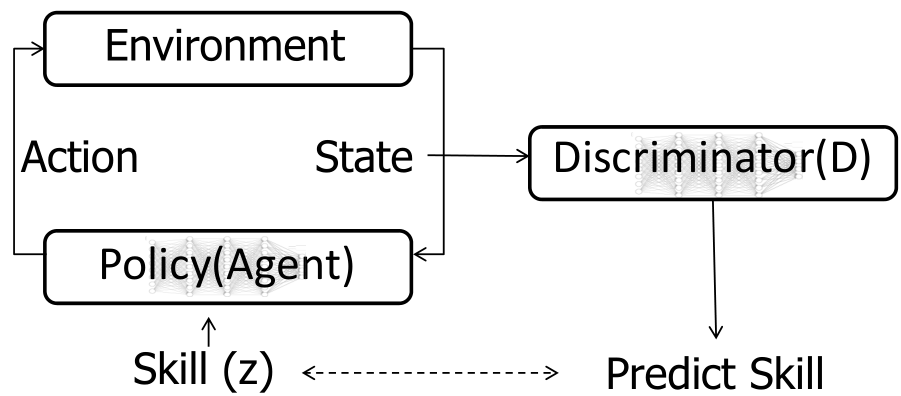
\includegraphics[width=.7\textwidth]{diayn.png}
	\caption{Diversity is All You Need. \cite{eysenbach2018diversity}.}
\end{figure}

\hlb{Connection to mutual information}
\begin{equation}
	\mathcal{I}(z,\textbf{s}) = \mathcal{H}(z) - \mathcal{H}(z|\textbf{s})
\end{equation}
\begin{itemize}
	\item $\mathcal{H}(z)$: maximized by using uniform prior $p(z)$
	\item $\mathcal{H}(z|\textbf{s})$: minimized by maximizing $r(\textbf{s}, z) = \log p(z|\textbf{s})$
\end{itemize}

\section{References}
\begin{itemize}
	\item \citeaustitle{schmidhuber1991possibility}
	\item \citeaustitle{stadie2015incentivizing}
	\item \citeaustitle{osband2016deep}
	\item \citeaustitle{houthooft2016vime}
	\item \citeaustitle{bellemare2016unifying}
	\item \citeaustitle{tang2017exploration}
	\item \citeaustitle{fu2017ex2}
\end{itemize}
% !TeX spellcheck = en_US
\chapter{Control as Inference}

\begin{itemize}
	\item \textit{Inference} means the process of inferring something, or a conclusion reached on the basis of evidence and reasoning.	
	\item \textit{Probabilistic inference} is the task of deriving the \ac{prob} of one or more random variables taking a specific value or set of values.
	\item \textit{Variational inference} lets us approximate a high-dimensional Bayesian posterior with a simpler variational distribution by solving an optimization problem.
\end{itemize}

\section{Probabilistic Graphical Model}
\label{sec:probabilistic-graphical-model}
Good behavior most of the time has minor mistakes here and there, though overall it is optimal. Thus, good behavior is rather suboptimal. Traditional optimal control doesn't not consider stochastic suboptimal behaviors like that.

\begin{itemize}
	\item Traditional probabilistic model of optimal control
	\begin{align*}
		&\textbf{a}_1, \dots, \textbf{a}_T = \underset{\textbf{a}_1, \dots, \textbf{a}_T}{\arg\max} \sum_{t=1}^T r(\textbf{s}_t, \textbf{a}_t)\\
		&\textbf{s}_{t+1} = f(\textbf{s}_t, \textbf{a}_t)
	\end{align*}	
	\item Probabilistic graphical model: $\mathcal{O}_t$ as the optimality variable
	\begin{align}
		p(\textbf{s}_{1:T}, \textbf{a}_{1:T}) &= p(\tau)\\
		p(\mathcal{O}| \textbf{s}_t, \textbf{a}_t) &= \exp (r(\textbf{s}_t, \textbf{a}_t))\\
		p(\tau | \mathcal{O}_{1:T}) &= \frac{p(\tau, \mathcal{O}_{1:T})}{p(\mathcal{O}_{1:T})}\\
		&\propto p(\tau) \prod_t \exp (r(\textbf{s}_t, \textbf{a}_t)) = p(\tau) \exp \left( \sum_t r(\textbf{s}_t, \textbf{a}_t) \right)
	\end{align}
	\begin{center}
		\begin{tikzpicture}[roundnode/.style={circle, draw=black!60, very thick, minimum size=7mm}]
			\node[roundnode](s1){$\textbf{s}_1$};
			\node[roundnode](s2)[right=3cm of s1]{$\textbf{s}_2$};	
			\node[roundnode](s3)[right=3cm of s2]{$\textbf{s}_3$};
			\node[roundnode](a1)[above right=1cm and 0.2cm of s1]{$\textbf{a}_1$};
			\node[roundnode](a2)[above right=1cm and 0.2cm of s2]{$\textbf{a}_2$};
			\node[roundnode](a3)[above right=1cm and 0.2cm of s3]{$\textbf{a}_3$};
			\node[roundnode, fill=gray](o1)[above left=.9cm and .5cm of a1]{$\mathcal{O}_1$};
			\node[roundnode, fill=gray](o2)[above left=.9cm and .5cm of a2]{$\mathcal{O}_2$};
			\node[roundnode, fill=gray](o3)[above left=.9cm and .5cm of a3]{$\mathcal{O}_3$};
			\draw[-latex](s1.east) -- (s2.west) node[midway, below]{$p(\textbf{s'|s,a})$};
			\draw[-latex](s2.east) -- (s3.west);
			\draw[-latex](a1.south east) -- (s2.west);
			\draw[-latex](a2.south east) -- (s3.west);
			\draw[-latex](s1.north) -- (o1.south);
			\draw[-latex](s2.north) -- (o2.south);
			\draw[-latex](s3.north) -- (o3.south);
			\draw[-latex](a1.north west) -- (o1.south east);
			\draw[-latex](a2.north west) -- (o2.south east);
			\draw[-latex](a3.north west) -- (o3.south east);
			\draw[-latex](s3.east) -- (12,0);
			\draw[-latex](a3.south east) -- (12,0);
			\node at (13,0) {\LARGE \textbf{\dots}};
		\end{tikzpicture}
	\end{center}
\end{itemize}

\section{Control as Inference}
\label{sec:control-as-inference}

Here, \textit{inference} implies planning. To do inference, we compute the three following terms:
\begin{align*}
	&\beta_t (\textbf{s}_t, \textbf{a}_t) = p(\mathcal{O}_{t:T}| \textbf{s}_t, \textbf{a}_t) && -\text{backward messages}\\
	&p(\textbf{a}_t | \textbf{s}_t, \mathcal{O}_{1:T}) && -\text{policy}\\
	&\alpha_t(\textbf{s}_t) = p(\textbf{s}_t | \mathcal{O}_{1:t-1}) && -\text{forward messages}\\
\end{align*}

\subsection{Backward Messages Computation}
Backward messages $\beta_t (\textbf{s}_t, \textbf{a}_t) = p(\mathcal{O}_{t:T}| \textbf{s}_t, \textbf{a}_t)$ is the \ac{prob} of optimality from the current time step $t$ till the end $T$, given the current state. $\textbf{s}_t$ and action $\textbf{a}_t$.
\begin{align*}
	\beta_t (\textbf{s}_t, \textbf{a}_t) &= p(\mathcal{O}_{t:T}| \textbf{s}_t, \textbf{a}_t) && -\text{the state-action backward message}\\
	\beta_t (\textbf{s}_t) &= p(\mathcal{O}_{t:T}| \textbf{s}_t) && -\text{the state backward message}
\end{align*}

Given:
\begin{align*}
	&p(\mathcal{O}_t| \textbf{s}_t, \textbf{a}_t) \propto \exp (r(\textbf{s}_t, \textbf{a}_t)) && \text{\ac{prob} of current optimality given state and action}\\
	&p(\textbf{s}_{t+1} | \textbf{s}_t, \textbf{a}_t) && \text{transition \ac{prob}}
\end{align*}

Formulation:
\begin{align}
	\beta_t (\textbf{s}_t, \textbf{a}_t)
	&= p(\mathcal{O}_{t:T}| \textbf{s}_t, \textbf{a}_t)\\
	&= \int p(\mathcal{O}_{t:T}, \textbf{s}_{t+1}| \textbf{s}_t, \textbf{a}_t) d\textbf{s}_{t+1}\\
	&= \int p(\mathcal{O}_{t+1:T}| \textbf{s}_{t+1}, \textbf{s}_t, \textbf{a}_t) p(\textbf{s}_{t+1} | \textbf{s}_t, \textbf{a}_t) p(\mathcal{O}_t| \textbf{s}_t, \textbf{a}_t) d\textbf{s}_{t+1}\\
	&= \int p(\mathcal{O}_{t+1:T}| \textbf{s}_{t+1}) \underbrace{p(\textbf{s}_{t+1} | \textbf{s}_t, \textbf{a}_t)}_{\text{known}} \underbrace{p(\mathcal{O}_t| \textbf{s}_t, \textbf{a}_t)}_{\text{known}} d\textbf{s}_{t+1}\\
	&= p(\mathcal{O}_t| \textbf{s}_t, \textbf{a}_t) \int p(\mathcal{O}_{t+1:T}| \textbf{s}_{t+1}) p(\textbf{s}_{t+1} | \textbf{s}_t, \textbf{a}_t)  d\textbf{s}_{t+1}\\
	\Rightarrow \beta_t (\textbf{s}_t, \textbf{a}_t)
	&= p(\mathcal{O}_t| \textbf{s}_t, \textbf{a}_t) \mathbb{E}_{\textbf{s}_{t+1} \sim p(\textbf{s}_{t+1} | \textbf{s}_t, \textbf{a}_t)} \left[ \beta_{t+1}(\textbf{s}_{t+1}) \right]\\
	p(\mathcal{O}_{t+1:T}| \textbf{s}_{t+1})
	&= \int \underbrace{p(\mathcal{O}_{t+1:T} | \textbf{s}_{t+1}, \textbf{a}_{t+1})}_{\text{backward message } \beta_{t+1} (\textbf{s}_{t+1}, \textbf{a}_{t+1})} \underbrace{p(\textbf{a}_{t+1} | \textbf{s}_{t+1})}_{\text{action prior}} d\textbf{a}_{t+1}\\
	\Rightarrow \beta_t (\textbf{s}_t) &= \mathbb{E}_{\textbf{a}_t \sim p(\textbf{a}_t | \textbf{s}_t)} \left[ \beta_t (\textbf{s}_t, \textbf{a}_t) \right] \qquad \text{(assuming uniform action prior $p(\textbf{a}_t | \textbf{s}_t)$)}
\end{align}

Recursive algorithm:
\begin{align}
	&\beta_T(\textbf{s}_T, \textbf{a}_T) =  p(\mathcal{O}_T| \textbf{s}_T, \textbf{a}_T) = \exp (r(\textbf{s}_T, \textbf{a}_T))\\
	&\text{for }t = T-1 \rightarrow 1:\\
	&\quad\beta_t (\textbf{s}_t, \textbf{a}_t) = p(\mathcal{O}_t| \textbf{s}_t, \textbf{a}_t) \mathbb{E}_{\textbf{s}_{t+1} \sim p(\textbf{s}_{t+1} | \textbf{s}_t, \textbf{a}_t)} \left[ \beta_{t+1}(\textbf{s}_{t+1}) \right] \\
	&\quad\beta_t (\textbf{s}_t) = \mathbb{E}_{\textbf{a}_t \sim p(\textbf{a}_t | \textbf{s}_t)} \left[ \beta_t (\textbf{s}_t, \textbf{a}_t) \right]
\end{align}

\hlb{Further examination:}
\begin{align*}
	&\text{let}\; V_t(\textbf{s}_t) = \log \beta_t(\textbf{s}_t)\\
	&\text{let}\; Q_t(\textbf{s}_t, \textbf{a}_t) = \log \beta_t(\textbf{s}_t, \textbf{a}_t)\\
	&V_t(\textbf{s}_t) = \log \int \exp \big( Q_t(\textbf{s}_t, \textbf{a}_t) \big) d\textbf{a}_t\\
	&V_t(\textbf{s}_t) \rightarrow \underset{\textbf{a}_t}{\max} Q_t(\textbf{s}_t, \textbf{a}_t) \; \text{as $Q_t(\textbf{s}_t, \textbf{a}_t)$ gets bigger!} \Rightarrow \text{"soft max"}\\
	&Q_t(\textbf{s}_t, \textbf{a}_t) = r(\textbf{s}_t, \textbf{a}_t) + \log \mathbb{E} [\exp V_{t+1}(\textbf{s}_{t+1})]\\
	&Q_t(\textbf{s}_t, \textbf{a}_t) = r(\textbf{s}_t, \textbf{a}_t) + V_{t+1}(\textbf{s}_{t+1}) \quad \text{in case of deterministic transition}
\end{align*}
The above looks a lot like Bellman's equation $\Rightarrow$ $\log$ of $\beta_t$ is "Q-function-like"

\note Value functions are backward messages.

\subsection{The Action Prior}
Re-examine the action prior when computing the backward messages. Before, we assume it was uniform (as a constant to be ignored). If it's not uniform:

\begin{align}
	p(\mathcal{O}_{t+1:T}| \textbf{s}_{t+1}) &= \int \beta_{t+1} (\textbf{s}_{t+1}, \textbf{a}_{t+1}) p(\textbf{a}_{t+1} | \textbf{s}_{t+1}) d\textbf{a}_{t+1} = \beta_{t+1}(\textbf{s}_{t+1})\\
	\Rightarrow V(\textbf{s}_t) &= \log \int \exp \big( Q_t(\textbf{s}_t, \textbf{a}_t) + \log p(\textbf{a}_t | \textbf{s}_t) \big) d\textbf{a}_t = \log \beta_t(\textbf{s}_t) \\
	Q_t(\textbf{s}_t, \textbf{a}_t) &= r(\textbf{s}_t, \textbf{a}_t) + \log \mathbb{E} [\exp V_{t+1}(\textbf{s}_{t+1})] && \text{(before)}\\
	\widetilde{Q}_t(\textbf{s}_t, \textbf{a}_t) &= r(\textbf{s}_t, \textbf{a}_t) + \log p(\textbf{a}_t | \textbf{s}_t) + \log \mathbb{E} [\exp V_{t+1}(\textbf{s}_{t+1})] &&\text{(modified)}\\
	\Rightarrow V(\textbf{s}_t) &=  \log \int \exp \big( \widetilde{Q}_t(\textbf{s}_t, \textbf{a}_t)\big) d\textbf{a}_t
\end{align}
Thus, a simple modification to the reward will take account of the non-uniform action prior.\\
$\Rightarrow$ we can assume uniform action prior without loss of generality.

\subsection{Policy Computation}
\label{subsec:policy-computation}
The policy $p(\textbf{a}_t | \textbf{s}_t, \mathcal{O}_{1:T})$ is the current action \ac{prob} given the current state $\textbf{s}_t$ that the whole trajectory is optimal.

Given:
\begin{align*}
	&p(\mathcal{O}_t| \textbf{s}_t, \textbf{a}_t) \propto \exp (r(\textbf{s}_t, \textbf{a}_t)) && -\text{\ac{prob} of current optimality given state and action}\\
	&p(\textbf{s}_{t+1} | \textbf{s}_t, \textbf{a}_t) && -\text{transition \ac{prob}}\\
	&\beta_t (\textbf{s}_t, \textbf{a}_t) = p(\mathcal{O}_{t:T}| \textbf{s}_t, \textbf{a}_t) && -\text{backward messages}\\
	&\beta_t (\textbf{s}_t) = p(\mathcal{O}_{t:T}| \textbf{s}_t) && -\text{backward state messages}
\end{align*}

Formulation:
\begin{align}
	p(\textbf{a}_t | \textbf{s}_t, \mathcal{O}_{1:T})
	&= \pi(\textbf{a}_t | \textbf{s}_t) = p(\textbf{a}_t | \textbf{s}_t, \mathcal{O}_{t:T})\\
	&= \frac{p(\textbf{a}_t, \textbf{s}_t | \mathcal{O}_{t:T})}{p(\textbf{s}_t | \mathcal{O}_{t:T})}\\
	&= \frac{p(\mathcal{O}_{t:T} | \textbf{a}_t, \textbf{s}_t) p(\textbf{a}_t, \textbf{s}_t) / p(\mathcal{O}_{t:T})}{p(\mathcal{O}_{t:T} | \textbf{s}_t) p(\textbf{s}_t) / p(\mathcal{O}_{t:T})} \qquad\qquad\text{(Bayes rule)}\\
	&= \frac{p(\mathcal{O}_{t:T} | \textbf{a}_t, \textbf{s}_t)}{p(\mathcal{O}_{t:T} | \textbf{s}_t)} \frac{p(\textbf{a}_t, \textbf{s}_t)}{p(\textbf{s}_t)} = \frac{\beta_t (\textbf{s}_t, \textbf{a}_t)}{\beta_t (\textbf{s}_t)} p(\textbf{a}_t | \textbf{s}_t)\\
	\Rightarrow \pi(\textbf{a}_t | \textbf{s}_t) &= \frac{\beta_t (\textbf{s}_t, \textbf{a}_t)}{\beta_t (\textbf{s}_t)} \qquad\qquad \text{(assume uniform action prior $p(\textbf{a}_t | \textbf{s}_t)$=const)}
\end{align}

Recursive algorithm:
\begin{align}
	&\text{for }t = T-1 \rightarrow 1:\\
	&\quad Q_t(\textbf{s}_t, \textbf{a}_t) = r(\textbf{s}_t, \textbf{a}_t) + \log \mathbb{E} \left[ \exp ( V_{t+1}(\textbf{s}_{t+1}) ) \right]\\
	&\quad V_t(\textbf{s}_t) = \log \int \exp \big(Q_t(\textbf{s}_t, \textbf{a}_t) \big) d\textbf{a}_t
\end{align}

Policy computation with value functions:
\begin{align}
	\pi(\textbf{a}_t | \textbf{s}_t) &= \frac{\beta_t (\textbf{s}_t, \textbf{a}_t)}{\beta_t (\textbf{s}_t)} \quad \text{with}\;\begin{cases}
		V_t(\textbf{s}_t) = \log \beta_t (\textbf{s}_t)\\
		Q_t(\textbf{s}_t, \textbf{a}_t) = \log \beta_t (\textbf{s}_t, \textbf{a}_t)
	\end{cases}\\
	\Rightarrow \pi(\textbf{a}_t | \textbf{s}_t) &= \exp \big(Q_t(\textbf{s}_t, \textbf{a}_t) - V_t(\textbf{s}_t)\big) = \exp \big( A_t(\textbf{s}_t, \textbf{a}_t)\big)
\end{align}
$\Rightarrow$ Soft advantage function with temperature:
\begin{equation}
	\pi(\textbf{a}_t | \textbf{s}_t) = \exp \left(\frac{1}{\alpha} A_t(\textbf{s}_t, \textbf{a}_t)\right) \quad \begin{cases}
		\alpha \rightarrow 0:\; \text{more deterministic}\\
		\alpha \rightarrow 1:\; \text{classical inference framework}
\end{cases}
\end{equation}

\subsection{Forward Messages Computation}
The forward messages $\alpha_t(\textbf{s}_t) = p(\textbf{s}_t | \mathcal{O}_{1:t-1})$ is the \ac{prob} of the state $\textbf{s}_t$ given that all previous trajectory steps are so far optimal.

Given:
\begin{align*}
	&p(\mathcal{O}_t| \textbf{s}_t, \textbf{a}_t) \propto \exp (r(\textbf{s}_t, \textbf{a}_t)) && -\text{\ac{prob} of current optimality given state and action}\\
	&p(\textbf{s}_{t+1} | \textbf{s}_t, \textbf{a}_t) && -\text{transition \ac{prob}}\\
	&\alpha(\textbf{s}_1) = p(\textbf{s}_1) && -\text{usually known}
\end{align*}

Formulation:
\begin{align}
	\alpha(\textbf{s}_t) &= p(\textbf{s}_t | \mathcal{O}_{1:t-1})\\
	&= \int p(\textbf{s}_t, \textbf{s}_{t-1}, \textbf{a}_{t-1} | \mathcal{O}_{1:t-1}) d\textbf{s}_{t-1} d\textbf{a}_{t-1}\\
	&= \int p(\textbf{s}_t | \textbf{s}_{t-1}, \textbf{a}_{t-1}, \mathcal{O}_{1:t-1}) p(\textbf{a}_{t-1} |\textbf{s}_{t-1}, \mathcal{O}_{1:t-1}) p(\textbf{s}_{t-1} | \mathcal{O}_{1:t-1}) d\textbf{s}_{t-1} d\textbf{a}_{t-1} \\
	&= \int \underbrace{p(\textbf{s}_t | \textbf{s}_{t-1}, \textbf{a}_{t-1})}_{\text{given}} p(\textbf{a}_{t-1} |\textbf{s}_{t-1}, \mathcal{O}_{t-1}) p(\textbf{s}_{t-1} | \mathcal{O}_{1:t-1}) d\textbf{s}_{t-1} d\textbf{a}_{t-1}
\end{align}
\begin{align}
	p(\textbf{a}_{t-1} |\textbf{s}_{t-1}, \mathcal{O}_{t-1}) p(\textbf{s}_{t-1} | \mathcal{O}_{1:t-1}) &= \frac{p(\mathcal{O}_{t-1} | \textbf{s}_{t-1}, \textbf{a}_{t-1}) p(\textbf{a}_{t-1} | \textbf{s}_{t-1})}{p(\mathcal{O}_{t-1} | \textbf{s}_{t-1})} \frac{p(\mathcal{O}_{t-1} | \textbf{s}_{t-1}) p(\textbf{s}_{t-1} | \mathcal{O}_{1:t-2})}{p(\mathcal{O}_{t-1} | \mathcal{O}_{1:t-2})}\\
	&= \underbrace{p(\mathcal{O}_{t-1} | \textbf{s}_{t-1}, \textbf{a}_{t-1})}_{\text{given}} \underbrace{p(\textbf{a}_{t-1} | \textbf{s}_{t-1})}_{\text{action prior}} \frac{\overbrace{p(\textbf{s}_{t-1} | \mathcal{O}_{1:t-2})}^{\textstyle \alpha_{t-1}(\textbf{s}_{t-1})}}{p(\mathcal{O}_{t-1} | \mathcal{O}_{1:t-2})}
\end{align}

The state marginal:
\begin{align}
	p(\textbf{s}_t | \mathcal{O}_{1:T}) =& \frac{p(\textbf{s}_t, \mathcal{O}_{1:T}) }{p(\mathcal{O}_{1:T})} = \frac{\overbrace{p(\mathcal{O}_{t:T} | \textbf{s}_t)}^ {\textstyle \beta_t(\textbf{s}_t)} p(\textbf{s}_t, \mathcal{O}_{1:t-1} )} {p(\mathcal{O}_{1:T})}\\
	& \propto \beta_t(\textbf{s}_t)	\underbrace{p(\textbf{s}_t | \mathcal{O}_{1:t-1})}_{\textstyle \alpha_t(\textbf{s}_t)} p(\mathcal{O}_{1:t-1}) \propto \beta_t(\textbf{s}_t) \alpha_t(\textbf{s}_t)
\end{align}

\subsection{Forward / Backward Message Intersection}
\begin{figure}[hbt!]
	\centering
	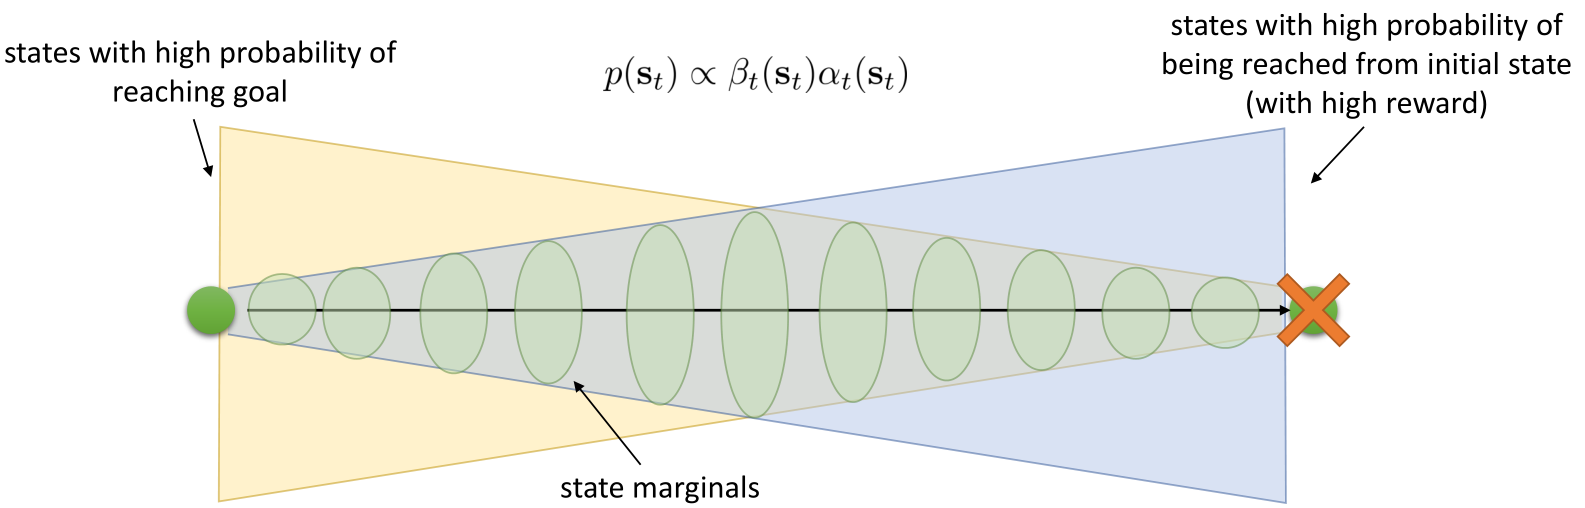
\includegraphics[width=.7\textwidth]{forward-backward-message-intersection.png}
	\caption{The intersection of backward and forward messages as state marginal (\href{http://rail.eecs.berkeley.edu/deeprlcourse/static/slides/lec-19.pdf}{UC Berkeley}).}
\end{figure}

\section{Control as Variational Inference}
\subsection{Optimism Problem}
The problem is due to the fact that given that you obtained high reward, the transition probability changes $p(\textbf{s}_{t+1} | \textbf{s}_t, \textbf{a}_t, \mathcal{O}_{1:T}) \neq p(\textbf{s}_{t+1} | \textbf{s}_t, \textbf{a}_t)$.
\begin{equation}
	Q_t(\textbf{s}_t, \textbf{a}_t) = r(\textbf{s}_t, \textbf{a}_t) + \underbrace{\log \mathbb{E} \left[ \exp ( V_{t+1}(\textbf{s}_{t+1}) ) \right]}_{\textstyle \text{"optimistic" transition}}
\end{equation}
Unlike in classic \ac{MDP}, the $\log$ of expectation of $\exp$ value function is overly optimistic, in the sense that a single large reward will overwhelm other values, while the average reward in expectation is low.

\hlb{Problem:} given that you obtained high reward, what was your action probability, \textit{given that your transition probability did not change?}

\hlb{Idea:} find a distribution $q(\textbf{s}_{1:T}, \textbf{a}_{1:T}) \approx p(\textbf{s}_{1:T}, \textbf{a}_{1:T} | \mathcal{O}_{1:T})$ but has dynamics $p(\textbf{s}_{t+1} | \textbf{s}_t, \textbf{a}_t)$

\subsection{Control via Variational Inference}
\begin{itemize}
	\item Let $\textbf{x} = \mathcal{O}_{1:T}$ and $z=(\textbf{s}_{1:T}, \textbf{a}_{1:T})$\\
	$\Rightarrow$ find $q(\textbf{z}) \approx p(\textbf{z}|\textbf{x})$
	\item Let $q(\textbf{z}) = q(\textbf{s}_{1:T}, \textbf{a}_{1:T}) = p(\textbf{s}_1) \prod_t p(\textbf{s}_{t+1} | \textbf{s}_t, \textbf{a}_t) q(\textbf{a}_t | \textbf{s}_t)$
\end{itemize}

The variational lower bound: $\log p(\textbf{x}) \geq \mathbb{E}_{\textbf{z} \sim q(\textbf{z})} [\log p(\textbf{x,z}) - \log q(\textbf{z})]$ (\href{AI_notes.pdf}{AI notes})
\begin{align*}	
	\Rightarrow \log p(\mathcal{O}_{1:T}) \geq \mathbb{E}_{(\textbf{s}_{1:T}, \textbf{a}_{1:T}) \sim q} \Bigg[ &\log p(\textbf{s}_1) + \sum_{t=1}^T \log p(\textbf{s}_{t+1} | \textbf{s}_t, \textbf{a}_t) + \sum_{t=1}^T \log p(\mathcal{O}_t | \textbf{s}_t, \textbf{a}_t) \\
	-&\log p(\textbf{s}_1) - \sum_{t=1}^T \log p(\textbf{s}_{t+1} | \textbf{s}_t, \textbf{a}_t) - \sum_{t=1}^T \log q(\textbf{a}_t | \textbf{s}_t) \Bigg]\\
	= \mathbb{E}_{(\textbf{s}_{1:T}, \textbf{a}_{1:T}) \sim q} \Bigg[ & \sum_t r(\textbf{s}_t, \textbf{a}_t) - \log q(\textbf{a}_t | \textbf{s}_t) \Bigg]\\
	= \sum_t \mathbb{E}_{(\textbf{s}_t, \textbf{a}_t) \sim q}  [r&(\textbf{s}_t, \textbf{a}_t) + \mathcal{H}(q(\textbf{a}_t | \textbf{s}_t))]
\end{align*}
$\Rightarrow$ This objective is the \ac{RL} objective, plus the action entropy. The additional action entropy term will give us more sub-optimal actions.

\hlb{Optimization with dynamic programming:}\\
- Base case: solve for the last time step $q(\textbf{a}_T | \textbf{s}_T)$
\begin{align*}
	q(\textbf{a}_T | \textbf{s}_T) &= \arg\max \mathbb{E}_{\textbf{s}_T \sim q (\textbf{s}_T)} \big[ \mathbb{E}_{\textbf{a}_T \sim q (\textbf{a}_T | \textbf{s}_T)} [r(\textbf{s}_T, \textbf{a}_T)] + \mathcal{H}(q(\textbf{a}_T | \textbf{s}_T)) \big]\\
	&= \arg\max \mathbb{E}_{\textbf{s}_T \sim q (\textbf{s}_T)} \big[ \mathbb{E}_{\textbf{a}_T \sim q (\textbf{a}_T | \textbf{s}_T)} [r(\textbf{s}_T, \textbf{a}_T) - \log q(\textbf{a}_T | \textbf{s}_T)] \big]
\end{align*}
Taking the derivative will result in: $q(\textbf{a}_T | \textbf{s}_T) \propto \exp(r(\textbf{s}_T, \textbf{a}_T))$
\begin{align}
	&q(\textbf{a}_T | \textbf{s}_T) = \frac{\exp (r(\textbf{s}_T, \textbf{a}_T))}{\int \exp(r(\textbf{s}_T, \textbf{a})) d\textbf{a}} = \exp \big( Q(\textbf{s}_T, \textbf{a}_T) - V(\textbf{s}_T) \big)\\
	&V(\textbf{s}_T) = \log \int \exp (Q(\textbf{s}_T, \textbf{a}_T)) d\textbf{a}_T\\
	\Rightarrow &\mathbb{E}_{\textbf{s}_T \sim q (\textbf{s}_T)} \big[ \mathbb{E}_{\textbf{a}_T \sim q (\textbf{a}_T | \textbf{s}_T)} [r(\textbf{s}_T, \textbf{a}_T) - \log q(\textbf{a}_T | \textbf{s}_T)] \big] = \mathbb{E}_{\textbf{s}_T \sim q (\textbf{s}_T)} \big[ \mathbb{E}_{\textbf{a}_T \sim q (\textbf{a}_T | \textbf{s}_T)} [V(\textbf{s}_T)] \big]
\end{align}
- At any time step: 
\begin{align*}
	Q_t(\textbf{s}_t, \textbf{a}_t) &= r(\textbf{s}_t, \textbf{a}_t) + \mathbb{E}[V_{t+1}(\textbf{s}_{t+1})] \qquad\text{(\textit{regular }Bellman backup - \textbf{not} optimistic)}\\
	q(\textbf{a}_t | \textbf{s}_t) &= \arg\max \mathbb{E}_{\textbf{s}_t \sim q (\textbf{s}_t)} \big[ \mathbb{E}_{\textbf{a}_t \sim q (\textbf{a}_t | \textbf{s}_t)} [r(\textbf{s}_t, \textbf{a}_t) + \mathbb{E}_{\textbf{s}_{t+1} \sim p(\textbf{s}_{t+1} | \textbf{s}_t, \textbf{a}_t)}[V(\textbf{s}_{t+1})]] + \mathcal{H}(q(\textbf{a}_t | \textbf{s}_t)) \big]\\
	&= \arg\max \mathbb{E}_{\textbf{s}_t \sim q (\textbf{s}_t)} \big[ \mathbb{E}_{\textbf{a}_t \sim q (\textbf{a}_t | \textbf{s}_t)} [Q(\textbf{s}_t, \textbf{a}_t)] + \mathcal{H}(q(\textbf{a}_t | \textbf{s}_t)) \big]\\
	&= \arg\max \mathbb{E}_{\textbf{s}_t \sim q (\textbf{s}_t)} \big[ \mathbb{E}_{\textbf{a}_t \sim q (\textbf{a}_t | \textbf{s}_t)} [Q(\textbf{s}_t, \textbf{a}_t) - \log q(\textbf{a}_t | \textbf{s}_t) ]\big]\\
	&\text{optimized when:}\; q(\textbf{a}_t | \textbf{s}_t) \propto \exp(Q_t(\textbf{s}_t, \textbf{a}_t))\\
	&V_t(\textbf{s}_t) = \log \int \exp(Q_t(\textbf{s}_t, \textbf{a}_t)) d\textbf{a}_t\\
	&q(\textbf{a}_t | \textbf{s}_t) = \exp \big( Q_t(\textbf{s}_t, \textbf{a}_t) - V_t(\textbf{s}_t) \big)
\end{align*}

Now we have a dynamic programming \ac{algor} for backward pass, \ac{aka} \textit{soft} value iteration \ac{algor}, which is similar to value iteration \ac{algor}:
\begin{align*}
	&\text{for}\; t=T-1 \rightarrow 1:\\
	&\quad Q_t(\textbf{s}_t, \textbf{a}_t) = r(\textbf{s}_t, \textbf{a}_t) + \mathbb{E}[V_{t+1}(\textbf{s}_{t+1})]\\
	&\quad V_t(\textbf{s}_t) = \log \int \exp(Q_t(\textbf{s}_t, \textbf{a}_t)) d\textbf{a}_t
\end{align*}

\begin{multicols}{2}
	Value iteration \ac{algor} (\secref{sec:value-iteration})
	\begin{enumerate}
		\item \tikzmark{via1}set $Q(\textbf{s,a}) \leftarrow r(\textbf{s,a}) + \gamma \mathbb{E}[V(\textbf{s}')]$
		\item \tikzmark{via2}set $V(\textbf{s}) \leftarrow \max_a Q(\textbf{s,a})$
		\begin{tikzpicture}[overlay,remember picture]
			\draw[very thick, -latex]
			([xshift=-7mm,yshift=1mm]pic cs:via2) --++ (-.5,0) |-
			([xshift=-7mm,yshift=1mm]pic cs:via1);
		\end{tikzpicture}
	\end{enumerate}
	\textit{Soft} value iteration \ac{algor} \cite{levine2018reinforcement}
	\begin{enumerate}
		\item \tikzmark{svia1}set $Q(\textbf{s,a}) \leftarrow r(\textbf{s,a}) + \gamma \mathbb{E}[V(\textbf{s}')]$
		\item \tikzmark{svia2}set $V(\textbf{s}) \leftarrow {\color{red}\text{soft} \max}_a Q(\textbf{s,a})$
		\begin{tikzpicture}[overlay,remember picture]
			\draw[very thick, -latex]
			([xshift=-7mm,yshift=1mm]pic cs:svia2) --++ (-.5,0) |-
			([xshift=-7mm,yshift=1mm]pic cs:svia1);
		\end{tikzpicture}
	\end{enumerate}
\end{multicols}

Variants:
\begin{itemize}
	\item Discounted SOC: $Q_t(\textbf{s}_t, \textbf{a}_t) = r(\textbf{s}_t, \textbf{a}_t) + {\color{red}\gamma} \mathbb{E} [V_{t+1}(\textbf{s}_{t+1})]$
	\item Explicit temperature: $V_t(\textbf{s}_t) = {\color{red}\alpha} \log \int \exp({\color{red}\frac{1}{\alpha}}Q_t(\textbf{s}_t, \textbf{a}_t)) d\textbf{a}_t$
\end{itemize}

\section{RL Algorithms as Inference}
Benefits of soft optimality
\begin{itemize}
	\item Improve exploration and prevent entropy collapse
	\item Easier to specialize (finetune) policies for more specific tasks
	\item Principled approach to break ties
	\item Better robustness (due to wider coverage of states)
	\item Can reduce to hard optimality as reward magnitude increases
	\item Good model for modeling human behavior
\end{itemize}

\subsection{Soft Q-Learning}
Q-Learning with Soft Optimality simply changes to the soft $\max$:
\begin{itemize}
	\item Standard Q-learning (\secref{sec:dql}):
	\begin{align*}
		&\phi \leftarrow \phi + \alpha \nabla_\phi Q_\phi(\textbf{s,a}) \big( r(\textbf{s,a}) + \gamma V(\textbf{s}') - Q_\phi(\textbf{s,a}) \big)\\
		&V(\textbf{s}') = \max_{\textbf{a}'} Q_\phi(\textbf{s}', \textbf{a}') && \text{(target value)}
	\end{align*}
	\item Soft Q-learning:
	\begin{align*}
		&\phi \leftarrow \phi + \alpha \nabla_\phi Q_\phi(\textbf{s,a}) \big( r(\textbf{s,a}) + \gamma V(\textbf{s}') - Q_\phi(\textbf{s,a}) \big) \\
		&V(\textbf{s}') = {\color{red}\text{soft} \max}_{\textbf{a}'} Q_\phi(\textbf{s}', \textbf{a}') = \log \int \exp \big( Q_\phi(\textbf{s}', \textbf{a}')\big) d\textbf{a}' && \text{(target value)}\\
		&\pi(\textbf{a}|\textbf{s}) = \exp \big( Q_\phi(\textbf{s,a}) - V(\textbf{s}) \big) = \exp \big(A_\phi(\textbf{s,a})\big)
	\end{align*}
	\begin{enumerate}
		\item \tikzmark{sql1}Take some action $\textbf{a}_i$ and observe $(\textbf{s}_i, \textbf{a}_i, \textbf{s}_i', r_i)$, add it to $\mathcal{R}$
		\item Sample mini-batch $\{(\textbf{s}_j, \textbf{a}_j, \textbf{s}_j', r_j) \}$ from $\mathcal{R}$ uniformly
		\item Compute $y_j = r_j + \gamma {\color{red}\text{soft} \max}_{\textbf{a}_j'} Q_{\phi'}(\textbf{s}_j', \textbf{a}_j')$ using \textit{target} network $Q_{\phi'}$
		\item $\phi \leftarrow \phi - \alpha \sum_j \frac{dQ_\phi}{d\phi}(\textbf{s}_j, \textbf{a}_j) \left( Q_{\phi}(\textbf{s}_j, \textbf{a}_j) - y_j \right)$
		\item \tikzmark{sql5}Update $\phi'$: copy $\phi$ every $N$ steps, or Polyak average $\phi' \leftarrow \tau \phi' + (1-\tau) \phi$
		\begin{tikzpicture}[overlay,remember picture]
			\draw[very thick, -latex]
			([xshift=-7mm,yshift=1mm]pic cs:sql5) --++ (-.5,0) |-
			([xshift=-7mm,yshift=1mm]pic cs:sql1);
		\end{tikzpicture}
	\end{enumerate}
\end{itemize}

\subsection{Entropy Regularized Policy Gradient}
Policy gradient with soft optimality:\\
$\pi(\textbf{a}|\textbf{s}) = \exp \big( Q_\phi(\textbf{s,a}) - V(\textbf{s}) \big)$ optimizes $J(\theta) = \sum_t \mathbb{E}_{\pi(\textbf{s}_t, \textbf{a}_t)} [r(\textbf{s}_t, \textbf{a}_t)] + \mathbb{E}_{\pi(\textbf{s}_t)} [\mathcal{H}(\pi(\textbf{a}_t | \textbf{s}_t))]$

\hlb{Intuition:}
\begin{align*}
	&\pi(\textbf{a}|\textbf{s}) \propto \exp ( Q_\phi(\textbf{s,a})) \;\text{when $\pi$ minimizes}\; D_{KL} \left( \pi(\textbf{a}|\textbf{s}) \Big|\Big| \frac{1}{Z} \exp (Q(\textbf{s,a}))\right) \\
	&D_{KL} \left( \pi(\textbf{a}|\textbf{s}) \Big|\Big| \frac{1}{Z} \exp (Q(\textbf{s,a}))\right) = \mathbb{E}_{\pi(\textbf{a|s})} [Q(\textbf{s,a})] -\mathcal{H}(\pi)
\end{align*}

\subsection{Soft Policy Gradient vs Soft Q-Learning}
Soft policy gradient derivation:
\begin{align}
	J(\theta) &= \sum_t \mathbb{E}_{\pi(\textbf{s}_t, \textbf{a}_t)} [r(\textbf{s}_t, \textbf{a}_t)] + \mathbb{E}_{\pi(\textbf{s}_t)} [\mathcal{H}(\pi(\textbf{a}_t | \textbf{s}_t))]\\
	&= \sum_t \mathbb{E}_{\pi(\textbf{s}_t, \textbf{a}_t)} [r(\textbf{s}_t, \textbf{a}_t) - \log \pi(\textbf{a}_t | \textbf{s}_t)]\\
	\nabla_\theta J &= \nabla_\theta \left[ \sum_t \mathbb{E}_{\pi(\textbf{s}_t, \textbf{a}_t)} [r(\textbf{s}_t, \textbf{a}_t) - \log \pi(\textbf{a}_t | \textbf{s}_t)] \right]\\
	&\approx \frac{1}{N} \sum_i \sum_t \nabla_\theta \log \pi(\textbf{a}_t | \textbf{s}_t) \Bigg( r(\textbf{s}_t, \textbf{a}_t) + \Bigg(\underbrace{\sum_{t'=t+1}^T r(\textbf{s}_{t'}, \textbf{a}_{t'}) - \log \pi(\textbf{a}_{t'} | \textbf{s}_{t'})}_{\textstyle \approx Q(\textbf{s}_{t+1}, \textbf{a}_{t+1})} \Bigg) - \log\pi(\textbf{a}_t | \textbf{s}_t) - \cancel{1} \Bigg)
\end{align}
We can ignore the $-1$ in the end (baseline).

Recall $\pi(\textbf{a}_t | \textbf{s}_t) = \exp \big(Q_t(\textbf{s}_t, \textbf{a}_t) - V_t(\textbf{s}_t)\big)$ (\subsecref{subsec:policy-computation}): 
\begin{equation}
	\nabla_\theta J(\theta) \approx \frac{1}{N} \sum_i \sum_t \big( \nabla_\theta Q_t(\textbf{s}_t, \textbf{a}_t) - \nabla_\theta V_t(\textbf{s}_t) \big) \big( r(\textbf{s}_t, \textbf{a}_t) + Q(\textbf{s}_{t+1}, \textbf{a}_{t+1}) - Q_t(\textbf{s}_t, \textbf{a}_t) + \cancel{V(\textbf{s}_t)} \big)
\end{equation}
Because of the baseline properties, any state dependent baseline can be removed, thus, we can ignore the $V(\textbf{s}_t)$.

Soft Q-learning (gradient descent, instead of gradient ascent in policy gradient):
\begin{equation}
	\nabla_\theta J(\theta) \approx - \frac{1}{N} \sum_i \sum_t \nabla_\theta Q_t(\textbf{s}_t, \textbf{a}_t) \big( r(\textbf{s}_t, \textbf{a}_t) + \underset{\textbf{a}_{t+1}}{\text{soft}\max} Q(\textbf{s}_{t+1}, \textbf{a}_{t+1}) - Q_t(\textbf{s}_t, \textbf{a}_t)\big)
\end{equation}

\section{Soft Actor-Critic}
Algorithm overview \cite{haarnoja2018soft}:
\begin{enumerate}
	\item Q-function update to evaluate current policy: this converges to $Q^\pi$
	\begin{equation}
		Q(\textbf{s,a}) \leftarrow r(\textbf{s,a}) + \mathbb{E}_{\textbf{s}' \sim p_\textbf{s}, \textbf{a}' \sim \pi} [Q(\textbf{s}', \textbf{a}') {\color{red} - \log \pi(\textbf{a}' | \textbf{s}')}]
	\end{equation}
	\item Update policy with gradient of information projection
	\begin{equation}
		\pi_{new} = \underset{\pi'}{\arg\min} D_{KL} \left( \pi'(\cdot | \textbf{s}) \Big|\Big| \frac{1}{Z} \exp Q^{\pi_{old}}(\textbf{s}, \cdot) \right)
	\end{equation}
	In practice, only take one gradient step on this objective
	\item Interact with the world, collect more data
\end{enumerate}

\section{References}
\begin{itemize}
	\item \citeaustitle{todorov2006linearly}
	\item \citeaustitle{todorov2008general}
	\item \citeaustitle{kappen2012optimal}
	\item \citeaustitle{ziebart2010modeling}
	\item \citeaustitle{rawlik2012stochastic}
	\item \citeaustitle{haarnoja2017reinforcement}
	\item \citeaustitle{nachum2017bridging}
	\item \citeaustitle{schulman2017equivalence}
	\item \citeaustitle{haarnoja2018soft}
	\item \citeaustitle{levine2018reinforcement}
\end{itemize}
% !TeX spellcheck = en_US
\chapter{Offline Reinforcement Learning}
\todo{}

\section{Overview}

The generalization gap

Definitions

\subsection{Fundamental Problem}
Distribution shift

\section{Batch RL via Importance Sampling}
\subsection{References}

\section{Batch RL via Linear Fitted Value Functions}

\section{Conservative Q-Learning}
\ac{CQL}

\section{Model-Based Offline RL}
\ac{MOPO}

\section{Summary}
\section{Applications}
\section{Open Questions}
% !TeX spellcheck = en_US
\chapter{Inverse Reinforcement Learning}

Prior to this, we have been manually design the reward function, which defines the task. There are cases, the reward function is unavailable or difficult to specify. The idea behind inverse \ac{RL} is to use human / expert's experience to \textit{learn} the reward function, then use it for \ac{RL} as a goal to optimize.

There is a difference between standard imitation learning and human imitation learning:
\begin{itemize}
	\item Standard imitation learning:
	\begin{itemize}
		\item copy the \textit{actions} performed by the expert
		\item no reasoning about outcomes of actions
	\end{itemize}	
	\item Human imitation learning:
	\begin{itemize}
		\item copy the \textit{intent} of the expert
		\item might take very different actions!
	\end{itemize}	
\end{itemize}

\section{Definition}
Inverse \ac{RL} \ac{vs} "forward" \ac{RL}:
\begin{center}
	\begin{tabular}[hbt!]{l|l}
		"Forward" \ac{RL} & Inverse \ac{RL} \\\hline\hline
		given: & given: \\
		states $s \in \mathcal{S}$, actions $a \in \mathcal{A}$ & states $s \in \mathcal{S}$, actions $a \in \mathcal{A}$\\
		(sometimes) transitions $p(\textbf{s}' | \textbf{s,a})$ & (sometimes) transitions $p(\textbf{s}' | \textbf{s,a})$\\
		reward function $r(\textbf{s,a})$ & samples $\{ \tau_i\}$ sampled from $\pi^*(\tau)$\\ \hline
		learn $\pi^*(\textbf{a}|\textbf{s})$ & learn $r_\psi(\textbf{s,a})$\\
		& \dots and then use it to learn $\pi^*(\textbf{a}|\textbf{s})$
	\end{tabular}
\end{center}

Choices for $\psi$:
\begin{itemize}
	\item linear reward function: $r_\psi(\textbf{s,a}) = \sum_i \psi_i f_i(\textbf{s,a}) = \psi^T \textbf{f}(\textbf{s,a})$
	\item neural net reward function: $r_\psi(\textbf{s,a})$
\end{itemize}

\section{Feature matching IRL}
\begin{itemize}
	\item Linear reward function: $r_\psi(\textbf{s,a}) = \sum_i \psi_i f_i(\textbf{s,a}) = \psi^T \textbf{f}(\textbf{s,a})$
	\item Let $\pi^{r_\psi}$ be the optimal policy for $r_\psi$, $\pi^*$ be the unknown optimal policy
	\item Pick $\psi$ such that $\mathbb{E}_{\pi^{r_\psi}}[\textbf{f}(\textbf{s,a})] = \mathbb{E}_{\pi^*} [\textbf{f}(\textbf{s,a})]$
\end{itemize}

\hlb{Problem:} still ambiguous

Maximum Margin Principle:
\begin{align*}
	&\underset{\psi, m}{\max}\; m &&\text{such that}\; \psi^T \mathbb{E}_{\pi^*}[\textbf{f}(\textbf{s,a})] \geq \underset{\pi \in \Pi}{\max} \psi^T \mathbb{E}_\pi [\textbf{f}(\textbf{s,a})] + m\\
	\Leftrightarrow &\underset{\psi}{\min} \frac{1}{2} ||\psi||^2 &&\text{such that}\; \psi^T \mathbb{E}_{\pi^*}[\textbf{f}(\textbf{s,a})] \geq \underset{\pi \in \Pi}{\max} \psi^T \mathbb{E}_\pi [\textbf{f}(\textbf{s,a})] + D(\pi, \pi^*) \quad\text{(\ac{SVM} trick)}
\end{align*}

\hlb{Issues:} \cite{abbeel2004apprenticeship, ratliff2006maximum}
\begin{itemize}
	\item Maximizing the margin is a bit arbitrary
	\item No clear model of expert suboptimality (can add slack variables…)
	\item Messy constrained optimization problem – not great for deep learning!
\end{itemize}

\section{MaxEnt IRL Algorithm}
Using the graphical model (\secref{sec:probabilistic-graphical-model}), we approach the problem as maximum likelihood learning: learning the \ac{param} $\psi$ to maximize the \ac{prob} of expert's trajectories given that they are (sub)optimal.
\begin{align}
	&p(\mathcal{O}_t | \textbf{s}_t, \textbf{a}_t, \psi) = \exp (r_\psi(\textbf{s}_t, \textbf{a}_t))\\
	&p(\tau | \mathcal{O}_{1:T}) = \frac{p(\tau, \mathcal{O}_{1:T})}{p(\mathcal{O}_{1:T})} \propto \cancel{p(\tau)} \exp \left( \sum_{t} r_\psi(\textbf{s}_t, \textbf{a}_t) \right) && (\text{$p(\tau)$ is independent of $\psi$})
\end{align}

The \ac{IRL}'s goal:
\begin{align}
	\psi =  \underset{\psi}{\arg\max} \frac{1}{N} \sum_{i=1}^N \log p(\tau_i | \mathcal{O}_{1:T}, \psi) = \underset{\psi}{\arg\max} \frac{1}{N} \sum_{i=1}^N r_\psi(\tau_i) - \log Z = \underset{\psi}{\arg\max} \mathcal{L}(\psi)
\end{align}

The \ac{IRL} partition function:
\begin{align}
	Z &= \int p(\tau) \exp(r_\psi(\tau)) d\tau \qquad\qquad (Z - \text{partition function})\\
	\nabla_\psi \mathcal{L} &= \frac{1}{N} \sum_{i=1}^N \nabla_\psi r_\psi(\tau_i) - \underbrace{\frac{1}{Z} \int p(\tau) \exp(r_\psi(\tau))}_{\textstyle p(\tau | \mathcal{O}_{1:T}, \psi)} \nabla_\psi r_\psi(\tau) d\tau\\
	&= \underset{\textstyle \text{expert samples}}{\mathbb{E}_{\tau \sim \pi^*(\tau)} [\nabla_\psi r_\psi(\tau_i)]} - \underset{\textstyle \text{soft optimal policy}}{\mathbb{E}_{\tau \sim p(\tau | \mathcal{O}_{1:T}, \psi)} [\nabla_\psi r_\psi(\tau)]} \label{eq:irl-goal}
\end{align}
The gradient is the difference between the expectation of the derivative of trajectory's reward between the expert's and the one from rolling out the current policy.

Estimation of the 2nd term:
\begin{align}
	\mathbb{E}_{\tau \sim p(\tau | \mathcal{O}_{1:T}, \psi)} [\nabla_\psi r_\psi(\tau)] &= \mathbb{E}_{\tau \sim p(\tau | \mathcal{O}_{1:T}, \psi)} \left[\nabla_\psi \sum_{t=1}^T r_\psi(\textbf{s}_t, \textbf{a}_t)\right]\\
	&= \sum_{t=1}^T \mathbb{E}_{(\textbf{s}_t, \textbf{a}_t) \sim p(\textbf{s}_t, \textbf{a}_t | \mathcal{O}_{1:T}, \psi)} [\nabla_\psi r_\psi(\textbf{s}_t, \textbf{a}_t)]\\
	p(\textbf{s}_t, \textbf{a}_t | \mathcal{O}_{1:T}, \psi) &= \underbrace{p(\textbf{a}_t | \textbf{s}_t, \mathcal{O}_{1:T}, \psi)}_{\textstyle \text{the policy}} \underbrace{p(\textbf{s}_t | \mathcal{O}_{1:T}, \psi)}_{\textstyle \text{the state marginal \ac{prob}}}
\end{align}
\begin{align*}
	&p(\textbf{a}_t | \textbf{s}_t, \mathcal{O}_{1:T}, \psi) = \frac{\beta(\textbf{s}_t, \textbf{a}_t)}{\beta(\textbf{s}_t)} \qquad\qquad
	p(\textbf{s}_t | \mathcal{O}_{1:T}, \psi) \propto \alpha(\textbf{s}_t) \beta(\textbf{s}_t) \qquad\qquad (\text{\secref{sec:control-as-inference}})\\
	\Rightarrow &p(\textbf{s}_t, \textbf{a}_t | \mathcal{O}_{1:T}, \psi) \propto \beta(\textbf{s}_t, \textbf{a}_t) \alpha(\textbf{s}_t) \qquad\qquad \text{let}\; \mu_t(\textbf{s}_t, \textbf{a}_t) \propto \beta(\textbf{s}_t, \textbf{a}_t) \alpha(\textbf{s}_t)
\end{align*}
\begin{align}
	\Rightarrow \mathbb{E}_{\tau \sim p(\tau | \mathcal{O}_{1:T}, \psi)} [\nabla_\psi r_\psi(\tau)] &= \sum_{t=1}^T \int\int \mu_t(\textbf{s}_t, \textbf{a}_t) \nabla_\psi r_\psi(\textbf{s}_t, \textbf{a}_t) d\textbf{s}_t d\textbf{a}_t = \sum_{t=1}^T \vec{\mu}_t \nabla_\psi \vec{r}_\psi
\end{align}

\ac{MaxEnt} \ac{IRL} Algorithm:
\begin{enumerate}
	\item \tikzmark{maxentirl1}Given $\psi$, compute backward message $\beta(\textbf{s}_t, \textbf{a}_t)$
	\item Given $\psi$, compute forward message $\alpha(\textbf{s}_t)$
	\item Compute $\mu(\textbf{s}_t, \textbf{a}_t) \propto \beta(\textbf{s}_t, \textbf{a}_t) \alpha(\textbf{s}_t)$
	\item Evaluate $\nabla_\psi \mathcal{L} = \frac{1}{N} \sum_{i=1}^N \sum_{t=1}^T \nabla_\psi r_\psi(\textbf{s}_{i,t}, \textbf{a}_{i,t}) - \sum_{t=1}^T \int\int \mu(\textbf{s}_t, \textbf{a}_t) \nabla_\psi r_\psi(\textbf{s}_t, \textbf{a}_t) d\textbf{s}_t d\textbf{a}_t$
	\item \tikzmark{maxentirl5}$\psi \leftarrow \psi + \eta \nabla_\psi \mathcal{L}$
	\begin{tikzpicture}[overlay,remember picture]
		\draw[very thick, -latex]
		([xshift=-7mm,yshift=1mm]pic cs:maxentirl5) --++ (-.5,0) |-
		([xshift=-7mm,yshift=1mm]pic cs:maxentirl1);
	\end{tikzpicture}
\end{enumerate}

\hlb{The name \ac{MaxEnt}:} when $r_\psi(\textbf{s}_t, \textbf{a}_t) = \psi^T \textbf{f}(\textbf{s}_t, \textbf{a}_t)$, the procedure optimizes $\underset{\psi}{\max} \mathcal{H}(\pi^{r_\psi})$ such that $\mathbb{E}_{\pi^{r_\psi}} [\textbf{f}] = \mathbb{E}_{\pi^*} [\textbf{f}]$. It is as random as possible while matching features. \cite{ziebart2008maximum}


\section{Guided Cost Learning Algorithm}
\hlb{Problems:} \ac{MaxEnt} \ac{IRL} so far requires:
\begin{itemize}
	\item Solving for (soft) optimal policy in the inner loop
	\item Enumerating all state-action tuples for visitation frequency and gradient
\end{itemize}

Practical problem settings:
\begin{itemize}
	\item Large and continuous state and action spaces
	\item States obtained via sampling only
	\item Unknown dynamics
\end{itemize}

\hlb{Idea:} learn $p(\textbf{a}_t | \textbf{s}_t, \mathcal{O}_{1:T}, \psi)$ using any $\max$ entropy \ac{RL} \ac{algor}, then run that policy to sample trajectories $\{\tau_j\}$
\begin{equation}
	\nabla_\psi \mathcal{L} \approx \frac{1}{N} \sum_{i=1}^N \nabla_\psi r_\psi(\tau_i) - \frac{1}{M} \sum_{j=1}^M \nabla_\psi r_\psi(\tau_j)
\end{equation}

If instead of expensively learning the policy, we just improve the policy (a little), we could use \textbf{\textit{importance sampling}} to handle the biased estimator. \cite{finn2016guided}
\begin{align}
	\nabla_\psi \mathcal{L} &\approx \frac{1}{N} \sum_{i=1}^N \nabla_\psi r_\psi(\tau_i) - \frac{1}{\sum_j w_j} \sum_{j=1}^M w_j \nabla_\psi r_\psi(\tau_j)\\
	w_j &= \frac{p(\tau) \exp(r_\psi(\tau_j))}{\pi(\tau_j)}\\
	&= \frac{\cancel{p(\textbf{s}_1)} \prod_t \cancel{p(\textbf{s}_{t+1} | \textbf{s}_t, \textbf{a}_t)} \exp(r_\psi(\textbf{s}_t, \textbf{a}_t))}{\cancel{p(\textbf{s}_1)} \prod_t \cancel{p(\textbf{s}_{t+1} | \textbf{s}_t, \textbf{a}_t)} \pi(\textbf{a}_t | \textbf{s}_t)} = \frac{\exp \big( \sum_t r_\psi(\textbf{s}_t, \textbf{a}_t) \big)}{\prod_t \pi(\textbf{a}_t | \textbf{s}_t)}
\end{align}

\section{IRL and GANs}
Similarity between \ac{IRL} and \ac{GAN}:
\begin{center}
	\begin{tabular}[hbt!]{p{8.5cm}|p{7.5cm}}
		\ac{IRL} & \ac{GAN} \cite{goodfellow2014generative} \\\hline\hline
		Player 1: policy $\pi_\theta$ & Player 1: the generator $p_\theta(\textbf{x|z})$\\
		Player 2: reward function $r_\psi$ & Player 2: the discriminator $p_\psi(\textbf{z|x})$ \\ \hline
		- The policy improves itself to make it \hlb{harder} to distinguish its samples and the expert demonstrations & - The generator improves itself to make it \hlb{harder} to distinguish its samples and the real images\\
		- The reward model improves itself to make it \hlb{easier} to distinguish the expert demonstrations and the policy's samples (\eqref{eq:irl-goal}) & - The discriminator improves itself to make it \hlb{easier} to distinguish the real images and the generator's samples
	\end{tabular}
\end{center}

\subsection{IRL as a GAN}
The optimal discriminator for \ac{GAN} is: $\displaystyle D^*(\textbf{x}) = \frac{p^*(\textbf{x})}{p_\theta(\textbf{x}) + p^*(\textbf{x})}$. For \ac{IRL}, optimal policy approaches $\pi_\theta(\tau) \propto p(\tau) \exp(r_\psi(\tau))$. Thus choosing parameterization for discriminator in the following way can remove importance weights (they are subsumed into $Z$) \cite{finn2016connection}
\begin{align}
	D_\psi(\tau) &= \frac{p(\tau)\frac{1}{Z}\exp(r(\tau))}{p_\theta(\tau) + p(\tau)\frac{1}{Z}\exp(r(\tau))} = \frac{\cancel{p(\tau)}\frac{1}{Z}\exp(r(\tau))}{\cancel{p(\tau)} \prod_t \pi_\theta(\textbf{a}_t | \textbf{s}_t) + \cancel{p(\tau)}\frac{1}{Z}\exp(r(\tau))}\\
	&= \frac{\frac{1}{Z}\exp(r(\tau))}{\prod_t \pi_\theta(\textbf{a}_t | \textbf{s}_t) + \frac{1}{Z}\exp(r(\tau))}\\
	\psi &\leftarrow \underset{\psi}{\arg\max} \mathbb{E}_{\tau \sim p^*} [\log D_\psi(\tau)] + \mathbb{E}_{\tau \sim \pi_\theta} [\log (1 - D_\psi(\tau))]
\end{align}

\subsection{Generative adversarial imitation learning}
We could also use regular discriminator ($D_\psi(\tau)$ as standard binary classifier) \cite{ho2016generative}.
\[\begin{matrix*}[l]
	\color{Green}+ \text{often simpler to set up optimization, fewer moving parts}\\
	\color{red}- \text{discriminator knows nothing at convergence}\\
	\color{red}- \text{generally cannot re-optimize the “reward”}
\end{matrix*}\]

\subsection{Generalization via IRL}
We need to decouple the \textbf{goal} from the \textbf{dynamics!} \cite{fu2017learning}

\section{References}
\hlb{Classic Papers:}
\begin{itemize}
	\item \citeaus{abbeel2004apprenticeship}. Apprenticeship learning via inverse reinforcement learning.
	\item \citeausm{ziebart2008maximum}. Maximum entropy inverse reinforcement learning.
\end{itemize}

\hlb{Modern Papers:}
\begin{itemize}
	\item \citeaus{finn2016guided}. Guided cost learning: Deep inverse optimal control via policy optimization.
	\item \citeaus{wulfmeier2015maximum}. Maximum entropy deep inverse reinforcement learning.
	\item \citeaus{ho2016generative}. Generative adversarial imitation learning.
	\item \citeaus{fu2017learning}. Learning robust rewards with adversarial inverse reinforcement learning.
\end{itemize}
% !TeX spellcheck = en_US
\chapter{Transfer and Multi-Task Learning}
If we’ve solved prior tasks, we might acquire useful knowledge for solving a new task. In \ac{RL}, knowledge is stored in:
\begin{itemize}
	\item Q-function: tells us which actions or states are good
	\item Policy: tells us which actions are potentially useful. Some actions are never useful!
	\item Models: what are the laws of physics that govern the world?
	\item Features/hidden states: provide us with a good representation
\end{itemize}

\section{Definitions}
\begin{itemize}
	\item \textit{Transfer learning} is using experience from \textit{\textbf{one set of tasks}} for faster learning and better performance on a \textit{\textbf{new task}} in \ac{RL}.
	\item In \ac{RL}, task = \ac{MDP}
	\item \textit{Shot}: number of attempts in the target domain
	\begin{itemize}
		\item 0-shot: just run the policy trained in the source domain
		\item 1-shot: try the task once
		\item few shot: try the task a few times
	\end{itemize}
\end{itemize}

No single solution!
\begin{itemize}
	\item Forward transfer: train on one task, transfer to a new task
	\begin{itemize}
		\item Transferring visual representations \& domain adaptation
		\item Domain adaptation in reinforcement learning
		\item Randomization
	\end{itemize}
	\item Multi-task transfer: train on many tasks, transfer to a new task
	\begin{itemize}
		\item Sharing representations and layers across tasks in multi-task learning
		\item Contextual policies
		\item Optimization challenges for multi-task learning
		\item Algorithms
	\end{itemize}
	\item Transferring models and value functions
	\begin{itemize}
		\item Model-based RL as a mechanism for transfer
		\item Successor features \& representations
	\end{itemize}	
\end{itemize}

\section{Forward Transfer}
\textit{Forward transfer}: train on one task, transfer to a new task.
\begin{itemize}
	\item Transferring visual representations \& domain adaptation
	\item Domain adaptation in reinforcement learning
	\item Randomization
\end{itemize}

Common challenges:
\begin{itemize}
	\item Domain shift: representations learned in the source domain might not work well in the target domain
	\item Difference in the \ac{MDP}: some things that are possible to do in the source domain are not possible to do in the target domain
	\item Finetuning issues: if pretraining \& finetuning, the finetuning process may still need to explore, but optimal policy during finetuning may be deterministic!
\end{itemize}

\subsection{Domain Adaptation}
\hlb{Invariance assumption:} everything that is \textbf{different} between domains is \textbf{irrelevant}.

\hlb{Idea:} force a representation layer (a layer) to be domain invariant.
$p(x)$ is different, exists some $z=f(x)$ such that $p(y|z) = p(y|x)$, but $p(z)$ is the same in both source and target domains. \cite{tzeng2020adapting}

Invariance is not enough when the dynamics don't match. \cite{eysenbach2020off}
\begin{align*}
	\tilde{r}(s,a) =& r(s,a) + \Delta r(s,a)\\
	\Delta r(s_t, a_t, s_{t+1}) =& \log p_{target}(s_{t+1} | s_t, a_t) - \log p_{source}(s_{t+1} | s_t, a_t)\\
	\Delta r(s_t, a_t, s_{t+1}) =& \log p(target | s_t, a_t, s_{t+1}) - \log p(target | s_t, a_t)\\
	&- \log p(source | s_t, a_t, s_{t+1}) - \log p(source | s_t, a_t)
\end{align*}
\hlb{Problems:}
\begin{itemize}
	\item The above approach considers limits in the target domain that doesn't present in source domain.
	\item But it doesn't consider things that can happen in target domain but limited in source domain.
\end{itemize}

\subsection{Finetuning}
Challenges:
\begin{itemize}
	\item RL tasks are generally much less diverse
	\begin{itemize}
		\item Features are less general
		\item Policies \& value functions become overly specialized
	\end{itemize}	
	\item Optimal policies in fully observed \ac{MDP}s are deterministic
	\begin{itemize}
		\item Loss of exploration at convergence
		\item Low-entropy policies adapt very slowly to new settings
	\end{itemize}	
\end{itemize}

Finetuning with maximum-entropy policies: act \hlb{as randomly as possible} while collecting high rewards. \cite{haarnoja2017reinforcement}

\subsection{References}
Domain adaptation:
\begin{itemize}
	\item \citeaustitle{tzeng2014deep}
	\item \citeaustitle{ganin2016domain}
	\item \citeaustitle{tzeng2020adapting}
	\item \citeaustitle{eysenbach2020off}
\end{itemize}

Finetuning:
\begin{itemize}
	\item \citeaustitle{haarnoja2017reinforcement}
	\item \citeaustitle{andreas2017modular}
	\item \citeaustitle{florensa2017stochastic}
	\item \citeaustitle{kumar2020one}
\end{itemize}

\section{Forward Transfer with Randomization}
\hlb{Idea:} If we can design the source domain, then vary it to prepare for the difficult in target domain.

\begin{itemize}
	\item Randomizing physical \ac{param} \cite{rajeswaran2016epopt}
	\item Explicit system identification \cite{yu2017preparing}
	\item Randomization for real-world control \cite{sadeghi2016cad2rl}
\end{itemize}

\subsection{References}
\begin{itemize}
	\item \citeaustitle{rajeswaran2016epopt}
	\item \citeaustitle{yu2017preparing}
	\item \citeaustitle{sadeghi2016cad2rl}
	\item \citeaustitle{tobin2017domain}
	\item \citeaustitle{james2017transferring}
	\item \citeaustitle{bousmalis2018using}
	\item \citeaustitle{rao2020rl}
\end{itemize}

\section{Multi-Task Transfer}
\hlb{Definition:} train on many tasks, transfer to a new task.
\begin{itemize}
	\item Sharing representations and layers across tasks in multi-task learning
	\item Contextual policies
	\item Optimization challenges for multi-task learning
	\item Algorithms
\end{itemize}

Multi-task \ac{RL} corresponds to a single-task \ac{RL} in a \hlb{joint \ac{MDP}}.

\hlb{Challenges:}
\begin{itemize}
	\item \hlb{Gradient interference:} becoming better on one task can make you worse on another\\
	\textit{Negative transfer} implies the transfer actually hurting the task's performance.
	\item \hlb{Winner-take-all problem:} imagine one task starts getting good algorithm is likely to prioritize that task (to increase average expected reward) at the expensive of others.
\end{itemize}

The two approaches is not really multi-task transfer. Not really fasten the learning speed of other tasks
\subsection{Actor-Mimic}
\begin{itemize}
	\item Train multiple single-task policy, then use supervised learning to combine them into one single policy. \cite{rusu2015policy}
	\item Analogous to guided policy search (\secref{sec:guided-policy-search}), but for transfer learning. \cite{levine2013icml}
\end{itemize}

\subsection{Policy Distillation}
Divide and Conquer does has some transfer between central policy and local policies, but not \hlb{much}. \cite{parisotto2015actor}

\subsection{Contextual Policies}
Can do (discern) multiple things in the same environment.
\begin{itemize}
	\item Standard policy: $\pi_\theta(\textbf{a|s})$
	\item Contextual policy: $\pi_\theta(\textbf{a|s}, \omega)$
	\item Augmented state space: $\tilde{\textbf{s}} = \begin{bmatrix}
		\textbf{s}\\
		\omega
	\end{bmatrix} \qquad \tilde{\mathcal{S}} = \mathcal{S} \times \Omega$
\end{itemize}

\section{Transferring Models and Value Functions}
\hlb{Assumption:}
\begin{itemize}
	\item the \textbf{dynamics} is the same in both domains
	\item but the \textbf{reward function} is different
\end{itemize}

\Eg:
\begin{itemize}
	\item Autonomous car learns how to drive to a few destinations, and then has to navigate to a new one.
	\item A kitchen robot learns to cook many different recipes, and
\end{itemize}

\subsection{Transferring Models}
Due to distribution shift, zero-shot might not always work. Although the dynamics is the same, they could be in different contexts: things present in source domain might not be present in target domain, and vice versa.

Unless the samples in the source domain is broad enough that they covers target domain's. 

\subsection{Transferring Value Functions}
Value functions couple dynamics, rewards, and policies, but in linearity.
\begin{equation}
	Q^\pi(\textbf{s,a}) = \underbrace{r(\textbf{s,a})}_{\textstyle \text{rewards}} + \gamma \mathbb{E}_{\textbf{s}' \sim \underbrace{p(\textbf{s}'|\textbf{s,a})}_{\textstyle \text{dynamics}}, \textbf{a}'\sim \underbrace{\pi(\textbf{a}'|\textbf{s}')}_{\textstyle \text{policies}}} [Q^\pi (\textbf{s}', \textbf{a}')]
\end{equation}

Let $\textbf{P}^\pi \textbf{v}$ denote a vector \textbf{w} of length $|S||A|$:
\begin{align}
	\textbf{w}(\textbf{s,a}) &= \mathbb{E}_{\textbf{s}' \sim p(\textbf{s}'|\textbf{s,a}), \textbf{a}'\sim \pi(\textbf{a}'|\textbf{s}')} [\textbf{v}(\textbf{s}', \textbf{a}')]\\
	\textbf{w}_{|S||A|\times 1} &= \textbf{P}^\pi_{|S||A|\times|S||A|} \textbf{v}_{|S||A|\times 1}\\
	Q^\pi &= r + \gamma \textbf{P}^\pi Q^\pi\\
	Q^\pi &= (\textbf{I} - \gamma \textbf{P}^\pi)^{-1} r
\end{align}

Let:
\begin{itemize}
	\item $\phi$ be an $|S||A| \times N$ \textit{feature} matrix
	\item $\psi$ be an $|S||A| \times N$ matrix such that $\psi = (\textbf{I} - \textbf{P}^\pi)^{-1}\phi$
	\item if $r=\phi w$, then $Q^\pi = \psi w$, with $w$ is a $1 \times N$ row vector\\
	In other words, if $r$ is a linear combination of $\phi$, then $Q^\pi$ is a linear combination of $\psi$
	\item $\psi_i$ is a "successor feature" for $\phi_i$
	\item for any \textit{new} reward function, if we can fit $r \approx \phi w$, we get $Q^\pi \approx \psi w$\\
	\note this holds for $Q^\pi$, not $Q^*$
	\[ Q^*(\textbf{s,a}) = r(\textbf{s,a}) + \gamma \mathbb{E}_{\textbf{s}' \sim p(\textbf{s}'|\textbf{s,a})}\left[ \underset{\textbf{a}'}{\max} Q^\pi(\textbf{s}', \textbf{a}') \right] \qquad \text{(no longer linear)}\]
\end{itemize}

\todo{} how to find $\psi, \phi$ given $\textbf{P}^\pi$

\hlb{Simplest use:} evaluation
\begin{enumerate}
	\item get small amount of data $(\textbf{s}_i, \textbf{a}_i, r_i, \textbf{s}_i')$ in new \ac{MDP}
	\item fit $w$ such that $\phi(\textbf{s}_i, \textbf{a}_i)w \approx r_i$ (linear regression)
	\item initialize $Q^\pi(\textbf{s,a}) = \psi(\textbf{s,a}) w$
	\item finetune $\pi$ and $Q^\pi$ with any \ac{RL} method
\end{enumerate}

\hlb{More sophisticated use:} train multiple $\psi^{\pi_i}$ functions for different $\pi_i$
\begin{itemize}
	\item choose initial policy $\pi(\textbf{s,a}) = \underset{\textbf{a}}{\arg\max} \psi^{\pi_i}(\textbf{s,a}) w$
	\item this provides a better initial policy in general
\end{itemize}

\hlb{Additional notes:} successor representations with $\phi = \textbf{I}$ \dots \cite{dayan1993improving}
% !TeX spellcheck = en_US
\chapter{Meta-Learning}

\section{Scaffolding}
\textit{Scaffolding} is a term that commonly used in the construction field, but also has a relation to infant's learning process. Scaffolding is a temporary structure that supports the construction, maintenance of a large building \href{https://en.wikipedia.org/wiki/Scaffolding}{(wiki)}. In the context of learning, it implies the structured assistance, or guidance, for better accomplishment of new skills and tasks. As the learner's \textit{autonomy} (learning abilities) increases, the support decrease accordingly . \cite{parentlab2019ccaffolding, zaadnoordijk2020next}

\begin{figure}[hbt!]
	\centering
	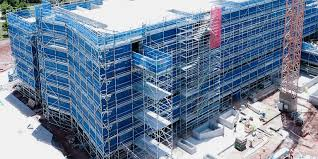
\includegraphics[width=.5\textwidth]{scaffolding.jpeg}
	\caption{Scaffolding in construction.}
\end{figure}

Extending the idea behind scaffolding to \ac{ML} and \ac{RL}: \cite{zaadnoordijk2020next}
\begin{itemize}
	\item Visual imitation learning \cite{finn2017one, sharma2019third}
	\item Learning from demonstration \todo{}
	\item Collective learning: learn from / guided by other agents
	\item Active learning
\end{itemize}

\todo{Read \cite{soltoggio2018born, arandjelovic2017look, barros2019expectation}}

\todo{Read \href{https://www.deepmind.com/publications/a-generalist-agent}{A Generalist Agent}}

\todo{Read \href{https://research.facebook.com/publications/control-strategies-for-physically-simulated-characters-performing-two-player-competitive-sports/}{meta}}

\section{Learning Resource}
\begin{itemize}
	\item \href{https://youtu.be/ByeRnmHJ-uk}{Learning to learn: An Introduction to Meta Learning || \ac{ICML} 2019}
\end{itemize}

\section{Definitions}
Conventional supervised learning relies on large and diverse dataset for broad generalization. There are, however, problems with limited labeled data. These scenarios would need a general purpose \ac{AI} system to adapt and learn on the job.

\begin{center}
	\begin{tabular}{p{8cm}|p{8cm}}
		Mechanistic view & Probabilistic view\\
		\hline\hline
		- Deep neural network model that can read in an entire dataset and make predictions for new datapoints  & - Extract prior information from a set of (meta-training) tasks that allows efficient learning of new tasks\\
		- Training this network uses a meta-dataset, which itself consists of many datasets, each for a different task & - Learning a new task uses this prior and (small) training set to infer most likely posterior parameters\\
		- Easier to implement meta-learning & - Easier to understand meta-learning
	\end{tabular}
\end{center}

\begin{itemize}
	\item If you’ve learned 100 tasks already, can you figure out how to learn more efficiently?
	\item Meta-learning = learning to learn
	\item In practice, very closely related to multi-task
	\item A meta-learned learner can:
	\begin{itemize}
		\item Explore more intelligently
		\item Avoid trying actions that are known to be useless
		\item Acquire the right features more quickly
	\end{itemize}
\end{itemize}

\section{Supervised Meta-learning}
The problem setup (\figref{fig:supervised-meta-learning}):
\begin{itemize}
	\item Meta-training: acquire your learned learning algorithm
	\item Meta-testing: use/adapt your learned learning algorithm
	\item Meta-training and meta-testing have separated training data and test data
\end{itemize}

\begin{figure}[hbt!]
	\centering
	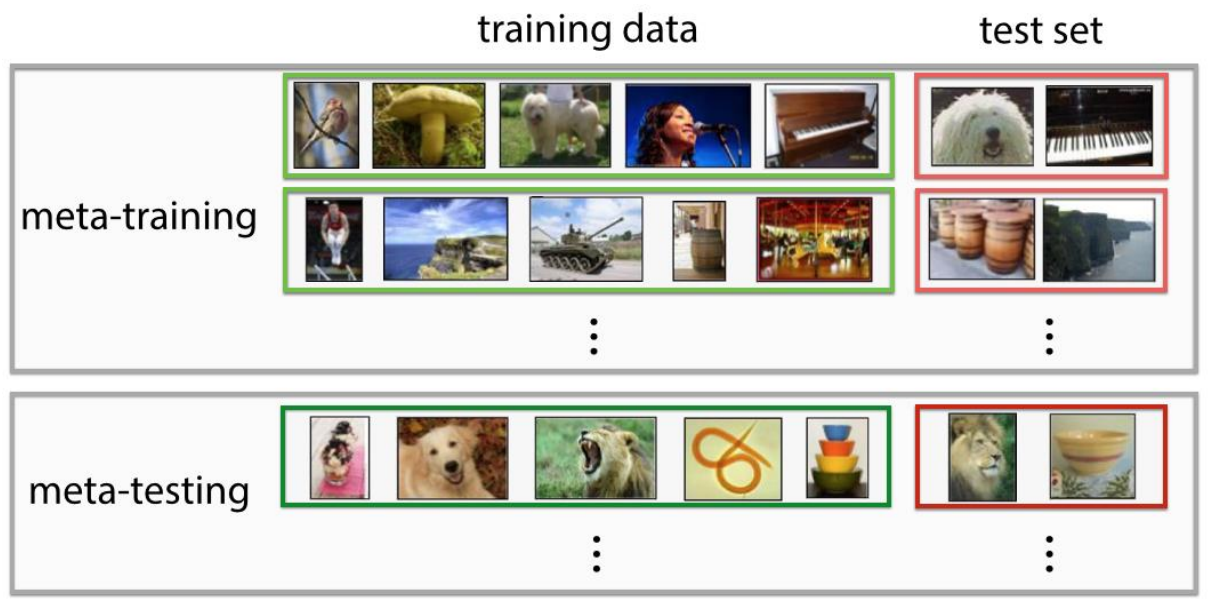
\includegraphics[width=.7\textwidth]{supervised-meta-learning.png}
	\caption{Supervised meta-learning pipeline (Ravi \& Larochelle '17)}
	\label{fig:supervised-meta-learning}
\end{figure}

\begin{multicols}{2}
	Supervised learning:
	\begin{align*}
		&f(x) \rightarrow y\\
		&\underset{\phi}{\arg\max} \log p(\phi | \mathcal{D})
	\end{align*}	
	Supervised meta-learning:
	\begin{align*}
		&f(\mathcal{D}^{tr}, x) \rightarrow y\\
		&\underset{\phi}{\arg\max} \log p(\phi | \mathcal{D}, \mathcal{D}_{meta-train})
	\end{align*}
\end{multicols}
\begin{align*}
	&x &&-\text{input}\\
	&y &&-\text{output}\\
	&\mathcal{D} = \{(x_1, y_1), \dots, (x_k, y_k)\} &&-\text{dataset}\\
	&\mathcal{D}_{meta-train} = \{(\mathcal{D}_1^{tr}, \mathcal{D}_1^{ts}), \dots, (\mathcal{D}_n^{tr}, \mathcal{D}_n^{ts})\} &&-\text{meta dataset}\\
	&\mathcal{D}_i = \{(x_1^i, y_1^i), \dots, (x_k^i, y_k^i)\}
\end{align*}

\begin{figure}[hbt!]
	\centering
	\begin{tikzpicture}[
		recnode1/.style={rectangle, draw=black!72, very thick, minimum width=1cm, minimum height=5mm},
		recnode2/.style={rectangle, minimum size=5mm}]
		\node[recnode1](x1){};
		\node[recnode1](x2)[right=of x1]{};
		\node[recnode1](x3)[right=of x2]{};
		\node[recnode1](x4)[right=of x3]{};
		\node[recnode2](y1)[below=0.5cm of x1]{$(x_1, y_1)$};
		\node[recnode2](y2)[below=0.5cm of x2]{$(x_2, y_2)$};
		\node[recnode2](y3)[below=0.5cm of x3]{$(x_3, y_3)$};
		\node[recnode2](y41)[below=0.5cm of x4]{$x_{test}$};
		\node[recnode2](y42)[above=0.5cm of x4]{$y_{test}$};
		\draw[-latex] (x1.east) -- (x2.west);
		\draw[-latex] (x2.east) -- (x3.west);
		\draw[-latex] (x3.east) -- (x4.west);
		\draw[-latex] (y1.north) -- (x1.south);
		\draw[-latex] (y2.north) -- (x2.south);
		\draw[-latex] (y3.north) -- (x3.south);
		\draw[-latex] (y41.north) -- (x4.south);
		\draw[-latex] (x4.north) -- (y42.south);
	\end{tikzpicture}
	\caption{Using \ac{RNN} to input a training set $\mathcal{D}^{tr}$, instead of just $x$.}
\end{figure}

The knowledge from the meta training dataset $\mathcal{D}_{meta-train}$ is extracted into parameter $\theta$:
\begin{align}
	&\theta^* = \underset{\theta}{\arg\max} \log p(\theta | \mathcal{D}_{meta-train}) && -\text{meta-learning} \\
	&\log p(\phi | \mathcal{D}, \mathcal{D}_{meta-train}) \approx \log p(\phi | \mathcal{D}, \theta^*)\\
	&\phi^* = \underset{\phi}{\arg\max} \log p(\phi | \mathcal{D}, \theta^*) && -\text{adaptation}
\end{align}

\begin{figure}[hbt!]
	\centering
	\begin{subfigure}[b]{0.45\textwidth}
		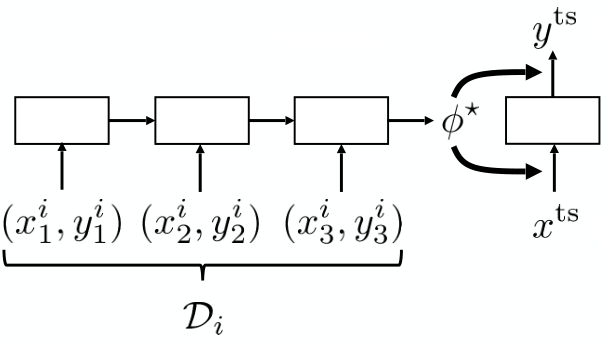
\includegraphics[width=\textwidth]{meta-training.png}
		\caption{Meta-training: $(x^{ts}, y^{ts}) \sim \mathcal{D}_i^{ts}$}
	\end{subfigure}
	\hfil
	\begin{subfigure}[b]{0.45\textwidth}
		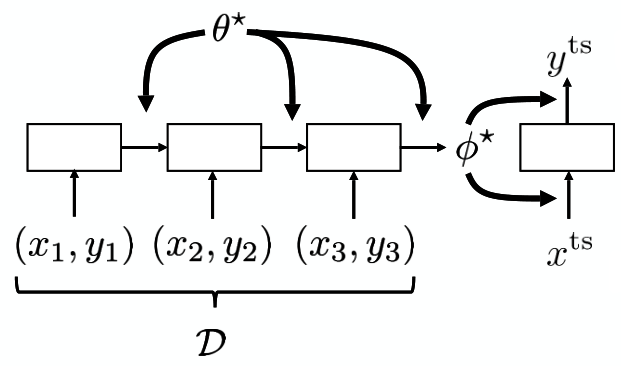
\includegraphics[width=\textwidth]{meta-testing.png}
		\caption{Meta-testing}
	\end{subfigure}
	\caption{Matching test and train conditions.}
\end{figure}

\begin{align}
	\phi^* = f_{\theta^*} (\mathcal{D}^{tr})
\end{align}

\todo{still confusing}

\begin{itemize}
	\item In meta-training, each task has a training set $\mathcal{D}^{tr}_i$ and a test set $\mathcal{D}^{ts}_i$.
	\item $\phi_i$ is the \ac{param} learned from the task's training set $\mathcal{D}^{tr}_i$ (\figref{fig:rnn-meta-learning}).\\
	$\phi_i = [h_i, \theta_p]$ with $h_i$ - \ac{RNN} hidden state, $\theta_p$ - meta-learned weights.
	\item In meta-testing, we optimize $\theta$, which is the $\arg\min$ of the average over all the tasks (in meta-training), of the loss of that task on its test set $\mathcal{D}^{ts}_i$.
\end{itemize}
\note The test set in meta-testing is not available (of course) for learning $\theta$, but the test set for meta-training is (\figref{fig:supervised-meta-learning}).

\begin{figure}[hbt!]
	\centering
	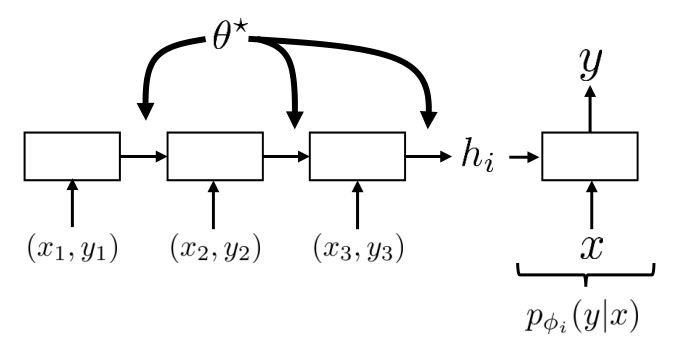
\includegraphics[width=.45\textwidth]{rnn-meta-learning.png}
	\caption{$\phi_i = [h_i, \theta_p]$ (\href{http://rail.eecs.berkeley.edu/deeprlcourse/static/slides/lec-22.pdf}{src})}
	\label{fig:rnn-meta-learning}
\end{figure}

\section{Meta Reinforcement Learning}
\begin{multicols}{2}
	Reinforcement learning:
	\begin{align*}
		\theta^* &= \underset{\theta}{\arg\min} \mathbb{E}_{\pi_\theta(\tau)} [R(\tau)]\\
		&= f_{RL}(\mathcal{M})\\
		&\mathcal{M} = \{\mathcal{S, A, P}, r\}:\;\text{the \ac{MDP}}
	\end{align*}
	Meta-reinforcement learning:
	\begin{align*}
		\theta^* &= \underset{\theta}{\arg\min} \sum_{i=1}^n \mathbb{E}_{\pi_{\phi_i}(\tau)} [R(\tau)]\\
		&\text{where}\; \phi_i = f_\theta(\mathcal{M}_i)\\
		&\mathcal{M}_i:\;\text{the \ac{MDP} for task $i$}
	\end{align*}
\end{multicols}

\begin{align}
	\mathcal{M}_i \sim p(\mathcal{M})\\
	\mathcal{M}_{test} \sim p(\mathcal{M})
\end{align}

\begin{itemize}
	\item In multi-task \ac{RL}, the context is typically given.
	\item In meta-\ac{RL}, the \textit{context} is inferred from experience from $\mathcal{M}_i$: $\pi_\theta(a_t | s_t, \phi_i)$
\end{itemize}

\section{Gradient-based Meta Learning}

\note The word \textit{agnostic} implies that some characteristics are irrelevant and that something is widely applicable. \Eg, a pick and place strategy is object-agnostic, if it doesn't matter what characteristics the object has, classes, geometries, materials, \etc. In other words, that strategy is compatible to a variety of objects.

\hlb{Idea:} pretraining as a type of meta-learning.\\
In \ac{MAML}, $f_\theta(\mathcal{M}_i)$ is itself an \ac{RL} \ac{algor} \cite{finn2017model}

\begin{align}
	\theta^* &= \arg\max \sum_{i=1}^n \mathbb{E}_{\pi_{\theta_i}} [r(\tau)]\\
	&\text{where}\; \phi_i = f_\theta(\mathcal{M}_i)\\
	f_\theta(\mathcal{M}_i) &= \theta + \alpha \nabla_\theta J_i(\theta)
\end{align}

\begin{align}
	&\cancel{\theta \leftarrow \theta + \alpha \nabla_\theta J(\theta)}\\
	&\theta \leftarrow \theta + \beta \sum_i \nabla_\theta J_i[\theta + \alpha \nabla_\theta J(\theta)]
\end{align}

\section{Meta-RL as a POMDP}
\subsection{PEARL}
\subsection{MELD}

\section{Model-Based Meta-RL}

\section{Meta-RL and Emergent Phenomena}
Humans and animals learn behaviors in a variety of ways. Perhaps each is a separate algorithm in the brain. But maybe these are all emergent phenomena resulting from meta-\ac{RL}:
\begin{itemize}
	\item Highly efficient but (apparently) model-free RL
	\item Episodic recall
	\item Model-based RL
	\item Causal inference
	\item etc.
\end{itemize}

References:
\begin{itemize}
	\item \citeausm{ritter2018been}. Been There, Done That: Meta-Learning with Episodic Recall.
	\item \citeausm{wang2018prefrontal}. Prefrontal Cortex as a Meta-Reinforcement Learning System.
	\item \citeausm{dasgupta2019causal}. Causal Reasoning from Meta-Reinforcement Learning.
\end{itemize}

\section{References}
\subsection{Gradient-based Meta-learning for RL}

\ac{MAML} meta-policy gradient estimators:
\begin{itemize}
	\item \citeaus{finn2017model}. Model-Agnostic Meta-Learning for Fast Adaptation of Deep Networks.
	\item \citeausm{foerster2018dice}. DiCE: The Infinitely Differentiable Monte Carlo Estimator.
	\item \citeausm{rothfuss2018promp}. ProMP: Proximal Meta-Policy Search.
\end{itemize}

Improving exploration:
\begin{itemize}
	\item \citeausm{gupta2018meta}. Meta-Reinforcement Learning of Structured Exploration Strategies.
	\item \citeausm{stadie2018some}. Some Considerations on Learning to Explore via Meta-Reinforcement Learning.
\end{itemize}
	
Hybrid algorithms (not necessarily gradient-based):
\begin{itemize}
	\item \citeausm{houthooft2018evolved}. Evolved Policy Gradients.
	\item \citeausm{fernando2018meta}. Meta-learning by the Baldwin effect.
\end{itemize}

\subsection{Meta-RL, Inference, and POMDPs}
\begin{itemize}
	\item \citeausm{rakelly2019efficient}. Efficient Off-Policy Meta-Reinforcement learning via Probabilistic Context Variables.
	\item \citeausm{zintgraf2019variational}. Variational Task Embeddings for Fast Adaptation in Deep Reinforcement Learning.
	\item \citeausm{humplik2019meta}. Meta reinforcement learning as task inference.
	\item \citeausm{liu2020explore}. Explore then Execute: Adapting without Rewards via Factorized Meta-Reinforcement Learning.
\end{itemize}

% !TeX spellcheck = en_US
\chapter{Continual Learning}
% !TeX spellcheck = en_US
\chapter{RL for Robotics}

\section{Motor Primitive Policy}
Not the same as path primitive from robotic trajectory planning. \cite{ijspeert2002movement}. Motor plans are trajectory plans for each \ac{dof}:
\begin{itemize}
	\item Spline-based trajectory plans: the desired movement is parameterized by its spline nodes and the duration of each spline node. \cite{miyamoto1995kendama, siciliano2008springer}
	\item Nonlinear dynamic motor primitives: the movement plans $(q_d, \dot{q}_d)$ are represented in terms of the time evolution of the nonlinear dynamical systems  \cite{ijspeert2002movement}
	\begin{align*}
		&\ddot{q}_d = f(q_d, z, g, \tau, \theta) \quad \text{in which:}\\
		&(q_d, \dot{q}_d) &&-\text{the desired position and velocity profile of a joint}\\
		&z &&-\text{the internal state $\ddot{z} = f_c(z,\tau)$}\\
		&\theta &&-\text{\ac{param} for $f$}\\
		&\tau &&-\text{the time duration shared by all \ac{dof}s}
	\end{align*}
\end{itemize}

We include exploration by adding a small perturbation to the desired accelerations
\begin{align}
	&\epsilon \sim \mathcal{N}(0, \sigma^2) &&-\text{small perturbation}\\
	&\ddot{\hat{q}}_d = \ddot{q}_d + \epsilon &&-\text{the perturbed target output}\\
	&\pi(\ddot{\hat{q}}_d | \ddot{q}_d) = \frac{1}{\sqrt{2\pi\sigma^2}} \exp\left( -\frac{(\ddot{\hat{q}}_d - \ddot{q}_d)^2}{2\sigma^2} \right) &&-\text{a stochastic policy}
\end{align}

\section{Requirements}
Requirements for motor primitive learning in robotics: \cite{peters2008nn}
\begin{itemize}
	\item Any change to the policy parameterization has to be smooth, because
	\begin{itemize}
		\item drastic changes can be hazardous for the robot and its environment
		\item rendering initialization of the policy based on domain knowledge or imitation learning useless, as these would otherwise vanish after a single update
		step due to out-of-distribution problem \cite{schaal1996learning}.
	\end{itemize}	
	\item Need to guarantee that the policy is improved in the update steps at least on average. This rules out greedy value function based methods with approximated value functions, as these methods are frequently problematic in regard of this property \cite{kakade2003sample}	
\end{itemize}

\section{References}
Resources:
\begin{itemize}
	\item \href{https://www.youtube.com/channel/UCXSgDUSFyJDDG3L1PcWq8Xg/featured}{EPHE 245 Motor Learning}
	\item \citeaustitle{schaal1996learning}
	\item \citeaustitle{ijspeert2002movement}
	\item \citeaustitle{kakade2003sample}
	\item \citeaustitle{peters2008nn}	
\end{itemize}
% !TeX spellcheck = en_US
\chapter{Challenges and Open Problems}

Multi-task transfer learning: deeper explanation for gradient interference and winner-take-all problem

\section{Stability}
\subsection{Problem}
\begin{itemize}
	\item Devising stable RL algorithms is very hard
	\item Q-learning/value function estimation
	\begin{itemize}
		\item Fitted Q/fitted value methods with deep network function estimators are typically not contractions, hence no guarantee of convergence
		\item Lots of parameters for stability: target network delay, replay buffer size, clipping, sensitivity to learning rates, etc.
	\end{itemize}	
	\item Policy gradient/likelihood ratio/REINFORCE
	\begin{itemize}
		\item Very high variance gradient estimator
		\item Lots of samples, complex baselines, etc.
		\item Parameters: batch size, learning rate, design of baseline
	\end{itemize}	
	\item Model-based RL algorithms
	\begin{itemize}
		\item Model class and fitting method
		\item Optimizing policy w.r.t. model non-trivial due to back-propagation
		\item More subtle issue: policy tends to exploit the model
	\end{itemize}
	\item How representative is your simulator? Usually the answer is "not very"
\end{itemize}
\subsection{Directions}
Can we develop more stable algorithms that are less sensitive to hyperparameters?
\begin{itemize}
	\item Algorithms with favorable improvement and convergence properties
	\begin{itemize}
		\item Trust region policy optimization \cite{schulman2015icml}
		\item Safe \ac{RL}, high-confidence policy improvement
	\end{itemize}
	\item Algorithms that adaptively adjust parameters
	\begin{itemize}
		\item Q-Prop: Sample-efficient policy gradient with an off-policy critic \cite{gu2016q}
	\end{itemize}
\end{itemize}

\section{Sample Complexity}
\subsection{Problem}
Efficiency: how long does it take to converge? (how many samples)
\begin{itemize}
	\item Real-world learning becomes difficult or impractical
	\item Precludes the use of expensive, high-fidelity simulators
	\item Limits applicability to real-world problems
\end{itemize}
\subsection{Directions}
\begin{itemize}
	\item Better model-based \ac{RL} algorithms
	\item Design faster algorithms
	\begin{itemize}
		\item Addressing Function Approximation Error in Actor-Critic Algorithms \cite{fujimoto2018addressing}
		\item Soft Actor-Critic \cite{haarnoja2018soft}
	\end{itemize}
	\item Reuse prior knowledge to accelerate reinforcement learning
	\begin{itemize}
		\item RL2: Fast reinforcement learning via slow reinforcement learning \cite{duan2016rl}
		\item Learning to reinforcement learning \cite{wang2016learning}
		\item Model-agnostic meta-learning \cite{finn2017model}
		\item DREAM \cite{liu2020explore}
	\end{itemize}
\end{itemize}

\section{Scaling and Generalization}
Off-policy and Offline \ac{RL}

\section{Problem Formulation}
\subsection{Single Task or Multi-Task}
We have the assumption that the trained tasks and the test task are from the same distribution. As the result, with enough trials, the agent will visit every possible situations. But in real world, it's never like that.

Prior works on generalizing from multi-task learning:
\begin{itemize}
	\item Train on multiple tasks, then try to generalize or finetune
	\begin{itemize}
		\item Policy distillation \cite{rusu2015policy}
		\item Actor-mimic \cite{parisotto2015actor}
		\item Model-agnostic meta-learning \cite{finn2017model}
	\end{itemize}
	\item Unsupervised or weakly supervised learning of diverse behaviors
	\begin{itemize}
		\item Stochastic neural networks \cite{florensa2017stochastic}
		\item Reinforcement learning with deep energy-based policies \cite{haarnoja2017reinforcement}
		\item Unsupervised information-theoretic exploration
	\end{itemize}
\end{itemize}

\subsection{Supervision}
\begin{itemize}
	\item If you want to learn from many different tasks, you need to get those tasks somewhere!
	\item Supervision comes from reward.
	\item Learn objectives/rewards from demonstration (inverse \ac{RL})
	\item Generate objectives automatically?
\end{itemize}

Unsupervised \ac{RL}
\begin{itemize}
	\item Interact with the world, without a reward function
	\item Learn something about the world (what?)
	\item Use what you learned to quickly solve new tasks
\end{itemize}
% !TeX spellcheck = en_US
\chapter{Technical Tools}

This chapter talks about or at least lists out helpful tools, platforms for working with \ac{RL}

\section{Supporting Platforms \& Tools}
Supporting platforms for simulation
\begin{itemize}
	\item MuJoCo
	\item \href{https://www.gymlibrary.ml/}{OpenAI \texttt{Gym}}: is a standard API for \ac{RL}, and a diverse collection of reference environments.
	\item \href{https://pybullet.org/wordpress/}{\texttt{PyBullet}}: physics simulation for games, visual effects, robotics and \ac{RL}.
\end{itemize}

\section{Coding Libraries}
\begin{itemize}	
	\item \href{https://github.com/deepmind/acme}{Acme}: DeepMind's research framework for \ac{RL}
	\item \href{https://www.tensorflow.org/agents/overview}{TensorFlow Agents}
	\item \href{https://github.com/openai/baselines}{OpenAI Baselines}: is a set of high-quality implementations of \ac{RL} algorithms.	
\end{itemize}
% !TeX spellcheck = en_US
\chapter{Research Proposal}

One major challenge in \ac{RL} is the ability to generalize to different tasks. For \ac{CV} with supervised learning, a model can be trained on a large dataset (\eg, ImageNet), then retrained on a smaller dataset to adapt with a specific task. This is possible because it was proven that early layers manage to learn different feature representations from the image. Thus, the feature extraction and inference process (based on that feature learning) can be separated. It is uncertain though, what a \ac{RL} model manages to learn in early layers.

What \ac{RL} differs from more conventional supervised learning are large diverse dataset, training procedure, how and when the data is collected, \etc. There are various proposed solution for \ac{RL} generalization problem: transfer learning, multi-task learning, meta-\ac{RL}. Offline \ac{RL} is one of those. It's strange though, as offline \ac{RL} aims to limit the interaction between the model and the world. Yet this interaction is what differs \ac{RL} with other \ac{AI} algorithms.

\section{Goal-oriented \ac{RL}}
Why the dataset is packed in the way transitions goes with rewards $\mathcal{D} = \{ (\textbf{s}_i, \textbf{a}_i, \textbf{s}_i', r_i) \}$. Prior works on single task have an underlying goal, from that goal, we have rewards for each state-action transition in the dataset. With different tasks, the rewards should be different, should the transition then goes with a certain goal. This is obvious in the multi-task setting. But even for single task setting, it's a bit strange because human's actions aren't often based on maximize rewards (keep running as far as we can, \etc). Even in business, we divide to quarterly objectives. Is it weird, even with discount factor or constrained reward windows? $\Rightarrow$ conditional \ac{RL} or task-oriented \ac{RL}. What if we remove the reward completely and just decide our actions based on desired goal and current state?

completely removing the reward is also the core idea behind imagined-goal-based exploration strategy, \etc. But what if we apply this idea to common \ac{RL} training and testing

\note
\begin{itemize}
	\item The reward can be seen as a representation for the goal.
	\item Eliminate all problems with value functions (overconfidence, \etc)
	\item Having a natural extension to multi-task learning
\end{itemize}

\subsection{Goal-oriented Imitation Learning}
A policy $\pi_\theta$ that is conditional on the goal $g$, take in state $\textbf{s}$ and output action $a$ (preferably joint configurations). The policy is optimized to copy the expert behaviors
\begin{equation}
	\pi_\theta(\textbf{a} | \textbf{s}, g)
\end{equation}

\subsection{Goal-oriented RL}
Same as above, but the policy is optimized not by maximize the reward, but by how far / different the goal state is, from the current state.

The prior reward is basically a representation of how different the goal state from the current state.

Would these solve the instability, overestimation problem of value-based \ac{RL} approaches?

\subsection{CGAN}
\ac{CGAN} idea:
\begin{itemize}
	\item Generator: $\textbf{a} = G(\textbf{s} | g)$
	\item Discriminator: $D(\textbf{s}, \textbf{a}, g) = good/bad?$
\end{itemize}

\todo{How is this relates to the notion of \textit{"context"} in the literature?}
	
\backmatter
\pagenumbering{Roman}
\printbibliography[heading=bibintoc]
\appendix
\end{document}